\documentclass[twoside,12pt]{Latex/Classes/PhDthesisPSnPDF}


%---------------------------------------------------------------
% Macros
% version 3 by Igor Ruiz-Agundez 2011
% version 2 by Jakob Suckale 2007
% version 1 by Harish Bhanderi 2002
%---------------------------------------------------------------

% This file contains macros that can be called up from connected TeX files
% It helps to summarise repeated code, e.g. figure insertion (see below).


%---------------------------------------------------------------
% MY COMMANDS
%---------------------------------------------------------------
\usepackage{bm} 
\usepackage{natbib}
%=========================================



%=========================================

%Times font and maths
%\usepackage{mathptmx}

%MY COMMANDS
%\documentclass[usenatbib]{mn2e} 
\newcommand{\sub}[1]{\mbox{\scriptsize{#1}}}
\newcommand{\der}[2]{ \frac{ \partial #1 }{\partial #2} }
\newcommand{\dtot}[2]{ \frac{ d #1 }{d #2} }
\newcommand{\pr}[1]{ \left( #1 \right) }
\newcommand{\cor}[1]{ \left[ #1 \right] }
\newcommand{\lla}[1]{ \left\{ #1 \right\} }
\newcommand{\eq}[2]{\begin{equation} \label{#1} #2 \end{equation}}
\newcommand{\bds}[1]{\boldsymbol{ #1 }}
\newcommand{\oiint}{\displaystyle\bigcirc\!\!\!\!\!\!\!\!\int\!\!\!\!\!\int}
\newcommand{\mathsize}[2]{\mbox{\fontsize{#1}{#1}\selectfont $#2$}}
\newcommand{\sinc}[1]{\mbox{sinc}#1}
\newcommand{\submath}[1]{\mbox{\scriptsize{#1}}}
\newcommand{\Msun}{h^{-1}\mbox{ M}_{\odot}}

\newcommand{\cita}[1]{\textsuperscript{\tiny\cite{#1}}}
\newcommand{\ket}{\rangle}
\newcommand{\bra}{\langle}

\AtBeginDocument{\renewcommand{\listtablename}{Índice de tablas}}
\AtBeginDocument{\renewcommand{\tablename}{Tabla}}

%\AtBeginDocument{\renewcommand{\ref}[1]{(\ref{#1})}}
%\renewcommand{\ref}[1]{(\ref{#1})}

\usepackage{color, colortbl}
%Celda de colores en tablas
\newcommand{\cellc}[1]{\multicolumn{1}{|>{\columncolor[rgb]{0.8, 0.8, 0.8}}c|}{#1}}

%New cite
%\AtBeginDocument{\renewcommand{\cite}[1]{(\citet{#1})}}

\newcommand{\LCDM}{$\Lambda$CDM}


%---------------------------------------------------------------
% Figures
%---------------------------------------------------------------


% Makes the \InsertFig macro compatible both with one or two columns
\makeatletter
\newlength \figwidth
\if@twocolumn
  \setlength \figwidth {\columnwidth}
\else
  \setlength \figwidth {\textwidth}
\fi
\makeatother

% \InsertFig allows inserting figures
% Parameters
% 1 --> Filename
% 2 --> Label for referencing
% 3 --> Title describing the figure (caption)
% 4 --> Description of the figure
% 5 --> Figure width, range [0,1]. If parameter is left blank the figure size is not change
% 6 --> Any other option for \includegraphics
% Usage:
% \InsertFig{}{}{}{}{}{}
%
\newcommand{\InsertFig}[6]{%
	\ifthenelse{\isempty{#5}}%
	{% if #1 is empty
		\begin{figure}[htbp!]
		\centering
		\includegraphics[#6]{#1}%
		\caption{#3}{\textbf{#4}}
		\label{#2}
		\end{figure}    
	}
	{% if #1 is not empty
		\begin{figure}[htbp!]
		\centering
		\includegraphics[width=#5\figwidth,#6]{#1}%
		\caption{#3}{\textbf{#4}}
		\label{#2}
		\end{figure}
	}
}

%% Simple version of \InsertFig
%\newcommand{\InsertFig}[5]{
%  \begin{figure}[htbp]
%   	\centering
%    \includegraphics[width=#4\textwidth,#5]{#1}%
%    \caption{#3}
%    \label{#2}
%  \end{figure}
%}



% insert a centered figure with caption
% parameters 1:filename, 2:label, 3:title, 
\newcommand{\figuremacro}[3]{
	\begin{figure}[htbp]
		\centering
		\includegraphics[width=1\textwidth]{#1}
		\caption[#3]{\textbf{#3}}
		\label{#2}
	\end{figure}
}


% insert a centered figure with caption and description
% parameters 1:filename, 2:label, 3:title, 4:description
\newcommand{\figuremacroD}[4]{
	\begin{figure}[htbp]
		\centering
		\includegraphics[width=1\textwidth]{#1}
		\caption[#3]{\textbf{#3} - #4}
		\label{#2}
	\end{figure}
}

% insert a centered figure with caption and description AND WIDTH
% parameters 1:filename, 2:label, 3:title, 4:description, 5: textwidth
% textwidth 1 means as text, 0.5 means half the width of the text
\newcommand{\figuremacroDW}[5]{
	\begin{figure}[htbp]
		\centering
		\includegraphics[width=#5\textwidth]{#1}
		\caption[#3]{\textbf{#3} - #4}
		\label{#2}
	\end{figure}
}

% inserts a figure with wrapped around text; only suitable for NARROW figs
% o is for outside on a double paged document; others: l, r, i(inside)
% text and figure will each be half of the document width
% note: long captions often crash with adjacent content; take care
% in general: above 2 macro produce more reliable layout
\newcommand{\figuremacroN}[3]{
	\begin{wrapfigure}{o}{0.5\textwidth}
		\centering
		\includegraphics[width=0.48\textwidth]{#1}
		\caption[#2]{{\small\textbf{#2} - #3}}
		\label{#1}
	\end{wrapfigure}
}




% Estas definiciones son para el comando \InsertFigBox
\newlength{\anchoFigura}
\newlength{\anchoFloat}
\addtolength{\fboxsep}{2\fboxsep}
%\renewcommand{\capfont}{\normalfont\normalcolor\sffamily\small}
%\renewcommand{\caplabelfont}{\normalfont\normalcolor\sffamily\bfseries\small}

% El comando \InsertFigBox nos permite insertar figuras en un marco
% Los parametros son:
% 1 --> Fichero de la imagen
% 2 --> Etiqueta (label) para referencias
% 3 --> Texto a pie de imagen
% 4 -> Porcentaje del ancho de página que ocupará la figura (de 0 a 1)
% 5 --> Opciones que queramos pasarle al \includegraphics
\newcommand{\InsertFigBox}[5]{%
  \setlength{\anchoFloat}{#4\textwidth}%
  \addtolength{\anchoFloat}{-4\fboxsep}%
  \setlength{\anchoFigura}{\anchoFloat}%
  \begin{figure}%
    \begin{center}%
      \Ovalbox{%
        \begin{minipage}{\anchoFloat}%
          \begin{center}%
            \includegraphics[width=\anchoFigura,#5]{#1}%
            \caption{#3}%
            \label{#2}%
          \end{center}%
        \end{minipage}
      }%
    \end{center}%
  \end{figure}%
}



%---------------------------------------------------------------
% Misc
%---------------------------------------------------------------

% predefined commands by Harish
\newcommand{\PdfPsText}[2]{
  \ifpdf
     #1
  \else
     #2
  \fi
}


%---------------------------------------------------------------
% Locales
%---------------------------------------------------------------


%%
%% Para quitar traducciones raras (Cuadros)
%% A de usarse cada vez que se seleccione el idioma
%%
\newcommand{\MejorarTraducciones}{%
       \renewcommand{\listtablename}{Índice de tablas}
       \renewcommand{\tablename}{Tabla}
       \renewcommand{\lstlistingname}{Lista}
}%



%---------------------------------------------------------------
% Source code
%---------------------------------------------------------------


%%
%% Para escribir extractos de codigo
%%
%% Las tabulaciones se substituyen por dos espacios
%\fvset{tabsize=2}
%% Creamos un nuevo environment de fancyvrb para los ejemplos enmarcados
%\DefineVerbatimEnvironment{VerbEj}{BVerbatim}{fontsize=\small,samepage=true,commandchars=\\\{\}}
%% Colo de fondo
%\definecolor{grisfondo}{gray}{0.9}
%% Environment para extractos de codigo
%\newenvironment{codigo}%
%{\VerbatimEnvironment\begin{Sbox}\begin{VerbEj}}%
%{\end{VerbEj}\end{Sbox}\setlength{\fboxsep}{8pt}\begin{center}\fcolorbox{black}{grisfondo}{\TheSbox}\end{center}}
%
%% Otro formato más bonito para código fuente
%\newcommand{\codigofuente}[3]{%
%  \lstinputlisting[language=#1,caption={#2}]{#3}%
%}






%: ----------------------------------------------------------------------
%:                  TITLE PAGE: name, degree,..
% -----------------------------------------------------------------------

% Title of the dissertation
\title{ALINEAMIENTO DE AGNs CON SU ENTORNO A GRAN ESCALA}


% ----------------------------------------------------------------------
% This section below defines front covert (external and internal)
% Shield logo
\crest{
\includegraphics[width=3cm]{figures/0_frontmatter/UdeA_Shield}}
% Full logo
%\crest{\includegraphics[width=6cm]{UDeusto}}
\university{Universidad de Antioquia \\ 
Facultad de Ciencias Exactas y Naturales \\ 
Instituto de Física}
\degree{}
\author{\textbf{Daniel Esteban Montenegro Taborda}} 
\collegeordept{Facultad de Ciencias Exactas y Naturales \\ 
Instituto de Física}
\textadvisor{}
\advisor{\textbf{Asesor:} Sebastian Bustamante-Jaramillo \\
\textbf{Co-asesor:} Juan C. Mu\~noz\ \ \ }
\textsignaturecandidate{Estudiante}
\textsignatureadvisor{Asesor\hspace{2.5 cm} Co-asesor}

\cityofbirth{Medellín}
%\degreedate{\monthname \ \the\year}
\degreedate{Noviembre \the\year}
% ----------------------------------------------------------------------
% turn of those nasty overfull and underfull hboxes
\hbadness=10000
\hfuzz=50pt

%Mejora Traducciones
\MejorarTraducciones


%: --------------------------------------------------------------
%:                  FRONT MATTER: dedications, abstract,..
% --------------------------------------------------------------

\begin{document}
\selectlanguage{spanish}
% sets line spacing
\renewcommand\baselinestretch{1.2}
\baselineskip=18pt plus1pt

\maketitle 

% Dedication
% Thesis Dedictation ---------------------------------------------------

\begin{dedication} %this creates the heading for the dedication page

\textit{Este trabajo esta dedicado a todas las mujeres que han aportado de alguna manera en mi vida M,J. En especial para mis amadas abuela y madre. Por su lucha incansable para que todo esto se hiciera posible.}

\end{dedication}

% ----------------------------------------------------------------------

% Title back
%% Thesis Titleback ---------------------------------------------------

\thispagestyle{empty}

\hfill

\vfill

\medskip


\noindent
\textit{
Alineamiento de AGNs con su entorno a gran escala
}




Autor: Daniel Montenegro

Asesor: Sebastian Bustamante-Jaramillo 

Co-asesor: Juan C. Mu\~noz 



\vfill

\vfill

\noindent
La siguiente página web contiene información actualizada sobre este trabajo y temas relacionados: \\
\url{https://github.com/Daniel-Montenegro/Thesis}


\noindent
Texto impreso en Medellín, Colombia

% TODO final date
\noindent
Primera Edici\'on, 
% Moth and year
\monthname \ \the\year

\vspace{1cm}
\hrule
\bigskip

% \cleardoublepage command ends the current page and causes all figures and tables that have so far appeared in the input to be printed. In a two-sided printing style, it also makes the next page a right-hand (odd-numbered) page, producing a blank page if necessary. 
\cleardoublepage

%%: ----------------------- cover page back side ------------------------
%% Your research institution may require reviewer names, etc.
%% This cover back side is required by Dresden Med Fac; uncomment if needed.
%
%\newpage
%\vspace{10mm}
%1. Reviewer: Name
%
%\vspace{10mm}
%2. Reviewer: 
%
%\vspace{20mm}
%Day of the defense:
%
%\vspace{20mm}
%\hspace{70mm}Signature from head of PhD committee:
%
%
%\cleardoublepage

% ----------------------------------------------------------------------

% The frontmatter text starts here
\frontmatter

%% Thesis Dedictation ---------------------------------------------------

\begin{dedication} %this creates the heading for the dedication page

\textit{Este trabajo esta dedicado a todas las mujeres que han aportado de alguna manera en mi vida M,J. En especial para mis amadas abuela y madre. Por su lucha incansable para que todo esto se hiciera posible.}

\end{dedication}

% ----------------------------------------------------------------------

%#########################################################################
%ABSTRACT


\begin{abstracts}
\selectlanguage{spanish}

%Los actuales desarrollos en los modelos de estructura del Universo a gran escala, observaciones y las \'ultimas simulaciones con un poder de resoluci\'on mayor, a su vez muestran un Universo distribuido en regiones (estructuras). Estas estructuras  se distribuyen de una manera compleja y en forma de filamentos. Dichos filamentos representan una sobre densidad de materia y son producto de la no linealidad del sistema. La estructura que conforman el universo se le denomina la red c\'osmica. \\

%La estructura del Universo plantea una duda que es el problema que se pretende resolver. ¿ Es posible encontrar una relaci\'on de las estructuras del Universo con las galaxias, o para ser m\'as específico con el spin de la misma?  Este trabajo nace la categorizaci\'on del mismo Universo, la particularidad de ciertas regiones da indicios de la relaci\'on entre entorno  galaxia; es por esto que se quiere conocer si la "mejor" relaci\'on es por parte del spin de las galaxias.

%La presencia(existencia) de las regiones(estructuras) son resultado de la evoluci\'on del universo. \\

%En estas regiones de sobre densidad se agrupan gran cantidad de materia que est\'a constituida por c\'umulos o agrupaciones de galaxias. Como su nombre lo dice, los c\'umulos o agrupaciones de galaxias son agrupaciones de galaxias debido a la interacci\'on gravitacional entre los cuerpos. Además, se conoce  la existencia de los agujeros negros al interior de las galaxias, el cual tiene asociado un spin. 

%La motivaci\'on de este trabajo es poder encontrar una relaci\'on entre  \\

%%%%%%%%%%%%%%%les  %%%%%%%%%%%%%%%%%%%%%%%%%%%%%%%%%%% un posible relaión entre el entorno ca%%%%%%%%%Las actuaobservaciones han venido demostrando
Los actuales estudios y observaciones han mostrado una posible relación entre la evolución del AGN y el entorno cosmológico al cual pertenece. En dirección de poder encontrar esta relación, este trabajo implementa la relación entre la orientación el espín del BH  hospedado en el AGN y la dirección del gradiente del campo de densidad del entorno. Para esto se usa un nuevo modelo de evolución de espín del BH, que incorpora además del régimen de acreción de gas coherente, usado en gran parte de las simulaciones actuales, el régimen de acreción de gas caótica, que representa te una manera general la evolución del espín del BH. Se realizan dos simulaciones magneto hidrodinámicas, en una se considera el régimen de acreción de gas caótico y en la otra el régimen de acreción de gas coherente, las dos con alta resolución y a un  $z=0$. 

Usando la relación entre la orientación del espín del BH ${\bf{J}_{bh}}$ y la orientación del autovector ${\bf{\vec{e}}_{3}}$, se encontró que la relación entre estos dos vectores $\cos\theta$ presenta una dependencia fuerte con la masa del BH. Se muestra que a medida que la masa del BH aumenta, $\cos\theta \to 0$, indicando una ortogonalidad entre el espín del BH y el gradiente del campo de densidad en función de la masa del BH. 







\end{abstracts}


%#########################################################################


%*************************************************************************
% Thesis Acknowledgements
%*************************************************************************
\begin{acknowledgements}      

.......

\begin{flushright}
\textit{Sinceramente,}


Daniel Montenegro


\monthname \ \the\year
\end{flushright}


\end{acknowledgements}

%*************************************************************************

%\selectlanguage{spanish}


\setcounter{secnumdepth}{5}
\setcounter{tocdepth}{5}

\tableofcontents

\listoffigures
%\listoftables



% this file is called up by thesis.tex
% content in this file will be fed into the main document

% Glossary entries are defined with the command \nomenclature{1}{2}
% 1 = Entry name, e.g. abbreviation; 2 = Explanation
% You can place all explanations in this separate file or declare them in the middle of the text. Either way they will be collected in the glossary.

% required to print nomenclature name to page header
\markboth{\MakeUppercase{\nomname}}{\MakeUppercase{\nomname}}

% ----------------------- contents from here ------------------------
%

%
%
%% acronyms


\nomenclature{LG}{Local Group}
\nomenclature{NGC}{New General Catalogue of Nebulae and Clusters of Stars}
\nomenclature{IC}{Index Catalogues}






\label{sec:glossary}

%: --------------------------------------------------------------
%:                  MAIN DOCUMENT SECTION
% --------------------------------------------------------------

\mainmatter

\pagestyle{fancy}



%------------------------- Introduction ------------------------
%qqqqqqqqqqqqqqqqqqqqqqqqqqqqqqqqqqqqqqqqqqqqqqqqqqqqqqqqqqqqqqqqqqqqqqqqq
%Quote
%\begin{savequote}[50mm]
%‘‘Equipado con sus cinco sentidos, el hombre explora el universo alrededor 
%suyo y llama a esta aventura Ciencia’’ 
%\qauthor{Edwin Hubble}
%\end{savequote}
%*************************************************************************




%#########################################################################
\chapter{Introducción}
\label{cha:Introduction}

Las observaciones del universo a gran escala nos inundan con una gran serie de dudas sobre el origen, constitución y el lugar que ocupamos en este inmenso universo. Nuestra necesidad de encontrar respuesta nos ha puesto en el lugar donde estamos, nos ha permitido desarrollar una ciencia que pretende encontrar respuestas, respuestas a tantas dudas. En la actualidad las observaciones a gran escala nos ha permitido evidenciar una organización, una distribución de materia que abarca todo el universo, constituida por un innumerable aglomeración de galaxias. Esta estructura  funciona además como conductos por donde fluye materia. Ahora, ¿ este flujo de materia altera la orientación de los objetos dentro de él ?
 
%-----------------------------------------
\section{Preliminares }
\label{sec: prelimenares}
%----------------------------------------
%El actual desarrollo de la ciencia nos permite obtener una cantidad absurda de información,  información que es de gran importancia a la hora de poder comprender el funcionamiento del universo. Es entonces tarea de la ciencia poder entender cómo funciona y por qué ocurren dichos eventos. En búsqueda de ello se ha desarrollado una serie de teorías, que van en dirección de explicar por qué y cómo se desarrollan las estructuras del universo, y reconocer los procesos que ocurren en él, procesos que son de gran importancia para el entendimiento de los procesos de formación y evolución en las galaxias.  
 
El posible alineamiento entre el flujo de materia que circula a través del espacio por regiones de sobre densidad, constituidas por galaxias, pueden proporcionar gran información para entender los procesos de formación de galaxias. En este trabajo se pretende determinar si existe alguna posible relación entre espín de Núcleos Activos de Galaxias (AGNs) con su entorno a gran escala. En la actualidad se ha desarrollado estudios observacionales que investigan la evolución de AGNs en diferentes regiones del espacio. Estos estudios han dado como resultado que el plano de polarización de la luz proveniente del AGN está alineada con la estructura local. A su vez, la dirección del plano de polarización está asociada con la orientación del espín del AGN \cite{hutsemekers2014}. Sin embargo debido a los impedimentos observacionales, donde solo es posible tomar un instante de tiempo, se hace necesario un modelo computacional que permita ver lo que ocurre en varios instantes, y con ello entender en gran medida los procesos evolutivos del AGN, en especial su orientación. Los resultados acá obtenidos tendrían consecuencias interesantes para el entendimiento de los procesos de formación de las galaxias, debido a que el espín del AGN esta íntimamente relacionados con procesos a muy grandes escalas, como formación de radio jets y ejección de masa por feedback del AGN, los cueles determinan propiedades fundamentales y globales de la galaxia anfitrión. 

%La teoría de formación de estructuras construidas a partir de las relatividad general y la cosmología, permiten reconstruir las observaciones, sin embargo se hace necesario realizar una serie de suposiciones. 

Las observaciones del universo a gran escala dejan ver una enmarañado sistema, una estructura que da cuenta de la distribución de materia y dinámica de la misma. La teoría de formación de estructuras \cite{zeldovich1970} permite reconstruir la forma del universo observable y proporciona un entendimiento de los sucesos que dan cabida a esta formación. Como ya se ha dicho, estas estructuras funcionan como conductos por donde la materia fluye. Estas estructuras son a su vez una constitución de galaxias que se agrupan bajo la acción de un potencial gravitacional, esta idea permite plantear un modelo de clasificación que faculte la distinción de entornos y poder estudiar la dinámica al interior de cada uno. Usando la teoría de sistemas dinámicos \cite{hahn2007}, se desarrolla una clasificación que parte de tensor de deformación del cual extrae los autovalores ($\lambda_{1}, \, \lambda_{1}, \, \lambda_{1}$), lo cuales proporcionan una criterio clasificación meramente dinámico, además se extrae los autovectores ($\vec{\bf{e_1}}$, $\vec{\bf{e_2}}$, $\vec{\bf{e_3}}$), que dan información de la orientación del flujo del campo de densidad. \cite{forero2009} desarrolla un método de clasificación para la red cósmica T-Web, que permite clasificar cada punto del espacio en los cuatros posibles entornos: voids, sheet, filament y clusters. 

La influencia del flujo de materia en el alineamiento del AGN solo es la primera parte del procesos de alineamiento. El modelo de espín estudia la evolución y alineamiento de los AGNs con procesos internos de la galaxia. \cite{fanidakis2011} desarrolla un modelo de evolución de espín, donde muestra la profunda relación que existe entre la tasa de acreción de materia y fusión de Agujero Negro (BH) con el espín. Sin embargo en este trabajo se va hacer uso de un modelo de evolución planteado por \cite{Bustamante2018b}. El cual incluye regímenes donde ocurren procesos de acreción caótica, esto al suponer modelos de auto-gravedad alrededor del disco de acreción del BH. 
 
Es entonces el propósito de este trabajo determinar a partir de simulaciones cosmológicas hidrodinámicas (Illustris TNG AGN+ physics model) \cite{springel2010}, y un modelo de evolución de espín de Agujeros Súper Masivos (SMBH) en AGNs, posibles relaciones entre la orientación del AGN y el entorno cosmológico al cual pertenece. Para  determinar la posible relación, se calcula el valor del ángulo entre el espín de los BHs ${\bf{J_{bh}}}$ y el autovector $\vec{\bf{e_3}}$ correspondiente a cada BH.

Este escrito se organiza de la siguiente manera. las secciones 2 y 3 abarca el marco teórico, en la sección 2 se abarca lo correspondiente a la Cosmología y la formación de estructura, la sección 3 a la teoría de los AGNs. La teoría usada para la evolución del espín se encuentra consignada en la sección \ref{cha:Modelo de Spin}. La explicación de los métodos y simulaciones usadas para la obtención de la evolución del espín del AGN y la clasificación de entorno, son presentados en la sección \ref{cha: Algoritmo y modelacion}. Por último los resultados más relevantes, los propósitos a futuro y la conclusiones son exhibidos en la sección \ref{cha:cosmic_web}.

%*************************************************************************

%---------------------- Theoretical Frame -----------------------

%qqqqqqqqqqqqqqqqqqqqqqqqqqqqqqqqqqqqqqqqqqqqqqqqqqqqqqqqqqqqqqqqqqqqqqqqq
%Quote
\begin{savequote}[65mm]
‘‘
El espacio dice cómo se mueve la materia.
La materia dice cómo se curva el espacio.
’’
\qauthor{J.A. Wheeler}
\end{savequote}
%qqqqqqqqqqqqqqqqqqqqqqqqqqqqqqqqqqqqqqqqqqqqqqqqqqqqqqqqqqqqqqqqqqqqqqqqq




%#########################################################################
\chapter{Cosmología y Formación de estructuras}
\label{cha:Theoretical Framework}

\section{Relatividad General en el ámbito cosmológico}
\label{sec:IsotropicAndHomogeneousUniverse}
%***********************************************************************
%En la naturaleza existen cuatro fuerzas fundamentales. 
Al considerar un sistema donde interactúan dos ó más cuerpos con masa, la fuerza que intermedia entre las partículas es la fuerza de la gravedad. Es por eso que cuando se pretende abordar el estudio de la dinámica de este tipo de interacciones se debe remitir a la teoría de la gravedad. En la actualidad la mejor forma de reproducir la dinámica a gran escala del Universo es haciendo uso de la teoría de la Relatividad de Albert Einstein.
%Cuando se pretende estudiar el funcionamiento del universo en general, se debe invocar la ciencia que se encarga de ello. La cosmología estudia la dinámica del universo, el origen, evolución y futuro del mismo.  %Cuando se introducen la teoría de la relatividad general esta empieza a ser parte de la física, pues las leyes que describen el universo como un todo son las mismas que determinan el funcionamiento de los sistemas que se encuentra adentro de él. Esta teoría se  sustenta por una base matemáticamente robusta que  puede predecir eventos y reproduce las observaciones. 

En el camino de estudiar la dinámica del universo, un  paso obligado es conocer las ecuaciones de Einstein y por ende conocer sus soluciones, que son de gran importancia, porque relacionan la estructura del espacio-tiempo con su contenido de materia y su energía. 
%Estas ecuaciones no pueden dar una solución general exacta, es entonces necesario introducir ....
La cosmología busca describir el funcionamiento del universo a muy grandes escalas, donde solo se consideran las contribuciones de las galaxias, estrellas y otros objetos de manera global y no sus efectos individuales, posibilitando la solución a las ecuaciones de Einstein.

Aunque la cosmología pueda describir los eventos a grandes escalas, es necesario introducir restricciones de simetría, que permitan reproducir el universo actual. Es por esto, que la cosmología parte de un principio y un postulado que son claves en la construcción de la teoría:  

- El principio cosmológico, que habla sobre la distribución de la materia en el Universo a escalas del orden de cientos de megapársecs. Si se toma un punto cualesquiera en el espacio, la distribución de materia alrededor de él será homogénea e isotrópico, e.i., desde cualquier punto del espacio, en cualquier dirección se va observar la misma distribución de materia 
\cite{janssen2013}. %Una forma más estricta de decir este principio es:\\

%{\bf{Principio cosmológico:}} {\textit{El cualquier momento, el universo es homogéneo e isótropo a muy grandes escalas.}} (Bert Janssen,2013,p. 207). \\

Cuando se cuenta con un espacio el cuál es homogéneo e isótropo, este espacio presenta un máximo de simetría.  Matemáticamente, se dice que la métrica es invariante bajo cualquier rotación o traslación. 

?`Qué tan cierto puede llegar a ser esto? ?`el universo sí es homogéneo e isótropo? Cuando se observa el universo, la materia tiende a estar concentrada, las estrellas se concentran en galaxias, las galaxias en cúmulos de galaxias y a su vez estos cúmulos en otros súper cúmulos. Entonces, ?`que tan cierto es que el universo sea homogéneo? Para tener un universo homogéneo e isótropo se debe considerar observaciones a una escala mucho mayor (en el orden de $300$ Mpcs), un ejemplo es la radiación cósmica de fondo, que corresponde a la radiación térmica proveniente del origen del universo, la cual tiene una anisotropía del orden de $\Delta T /T \sim 10^{-5}$\cite{bond1987}. 

\begin{center}
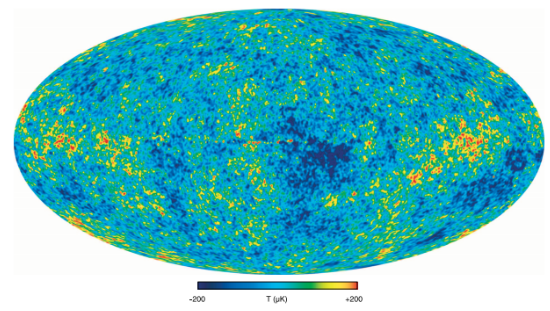
\includegraphics[scale=.5]{./figures/2_theoretical_framework/backgraundCosmicRadiation.png}
\figcaption[Mapa de las anisotropías]{\emph{Mapa de las anisotropías de la radiación cósmica del Universo  \cite{bennett2003}.}}\label{fig:radiación_cosmica_de_fondo}
\end{center}

- El postulado Weyl trata sobre la dinámica de las sobre densidades en el Universo, el cual enuncia que a escalas cosmológicas la materia se comporta como un fluido perfecto, que se mueve a lo largo de geodésicas temporales \cite{janssen2013}. %el cual dice: \\

%{\bf{Postulado de Weyl:}} {\textit{La materia a escalas cosmológicas se comporta como un fluido perfecto, cuyas componentes se mueven a lo largo de geodésicas temporales, que no se intersectan, salvo (posiblemente) en un punto en el pasado.}} (Bert Janssen,2013,p. 209)\\

El postulado de Weyl implica una idea muy importante en la cosmología, los observadores privilegiados. Estos observadores  se encuentran en reposo con respecto al fluido, lo cual implica que su movimiento es con respecto a la evolución del universo. El nombre que se le da a estos observadores es el de  observadores comóviles. Cuando se define este tipo de observadores también se define un tiempo cosmológico, que corresponde a la dirección temporal del observador comóvil. 



%*************************************************************************
%Geometría
\section{Geometría}
\label{sec:Geometría}
%***********************************************************************
En esta sección, se pretende abarcar el tema concerniente a la construcción matemática que hace posible describir la dinámica del universo. Se tomaron como referencia los libros: \cite{janssen2013}, \cite{longair2008}, \cite{baumann}. Si se desea profundizar en el tema, se recomienda seguir estos textos.
%---------------------------------------------------------------------
	%Metrica
	\subsection{La Métrica}
	\label{subsec:Metrica}
	%---------------------------------------------------------------------
	
En la relatividad general la métrica permite definir distancias, ángulos y volúmenes en una variedad de Riemann. Además juega un papel importante porque convierte las coordenadas dependientes del observador $X^{\mu}=(t,x^{i})$ en elementos de línea invariante


\begin{equation}
ds^{2}=\sum_{\mu,\nu}^{4} g_{\mu\nu}dX^{\mu}dX^{\nu} \equiv g_{\mu\nu}dX^{\mu}dX^{\nu} \,.
\label{eq:tensor_metrico}
\end{equation}

La métrica tiene una dependencia espacial y temporal $g_{\mu\nu}(t,{\bf{x}})$, entonces dependerá de donde se esté tomando y en que momento. Por esta dependencia espacio-temporal la métrica también dependerá de la distribución de la materia y la energía, debido a que esta debe reproducir los efectos de la gravedad.

La elección de la métrica responde al modelo del universo que se quiere describir. Para un universo homogéneo e isótropo se puede considerar un sistema con simetría esférica. La expresión para describir el diferencial de longitud entre dos puntos sobre la superficie de una esfera se escribe de la forma

\begin{equation}
dl^{2}=R_{c}^{2}d\theta^{2}+R_{c}^{2}\sin^{2}\theta d\phi^{2} \,,
\label{metrica_esfera}
\end{equation}
%
donde $R_{c}$ es el radio de curvatura de la esfera. La figura (\ref{fig:diferencial_linea_esferico}) presenta el diferencial de línea para una simetría esférica.


%------------------------------------------------------
\begin{center}
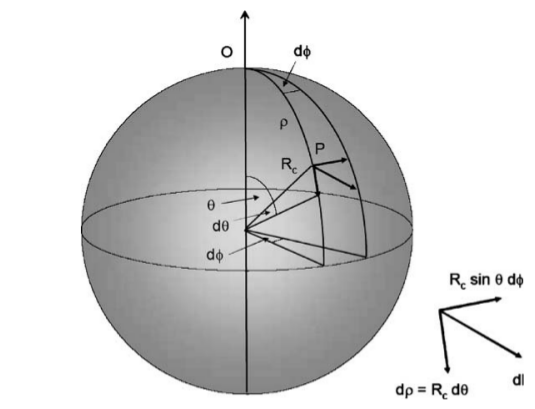
\includegraphics[scale=.4]{./figures/2_theoretical_framework/diferencial_linea.png}
\figcaption[diferencial de línea simetría esférica]{\emph{Representación del diferencial de línea para simetría esférica \cite{longair2008}.}}\label{fig:diferencial_linea_esferico}
\end{center}

%------------------------------------------------------

Usando la figura (\ref{fig:diferencial_linea_esferico}) se construye un arco $\rho$ entre los puntos O y P cuya distancia es $\rho=\theta R_{c}$, entonces la ecuación (\ref{metrica_esfera}) puede reescribirse de la forma

\begin{equation}
dl^{2}=d\rho^{2}+R_{c}^{2}\sin^{2}\left(\frac{\rho}{R_{c}} \right)d\phi^{2} \,.
\end{equation}
%
Una forma alternativa de escribir la métrica es introduciendo una distancia

\begin{equation}
x=R_{c}\sin\left(\frac{\rho}{R_{c}} \right) \,.
\end{equation}
%
Al calcular el diferencial y elevando al cuadrado se obtiene
%
\begin{equation}
dx^{2}=\left[1-\sin^{2}\left( \frac{\rho}{R_{c}}\right) \right]d\rho^{2}  \,, \hspace{1cm} d\rho^{2}=\frac{d^{2}}{1-kx^{2}} \,,
\end{equation}
%
donde $k=1/R_{c}^{2}$ es el parámetro de curvatura.

Por lo tanto la métrica se puede escribir de la forma 

\begin{equation}
dl^{2}=\frac{dx^{2}}{1-kx^{2}}+x^{2}d\phi^{2} \,.
\end{equation}

Se debe recordar que la constante de curvatura $k$ puede representar tres tipos de geometrías: Cuando se tiene una curvatura positiva se obtiene simetría esférica cerrada, con curvatura cero se obtiene el espacio Euclideo plano y si es negativo se tiene una geometría hiperbólica abierta. Ver figura (\ref{fig:curvatura_k}).\\

%-----------------------------------------
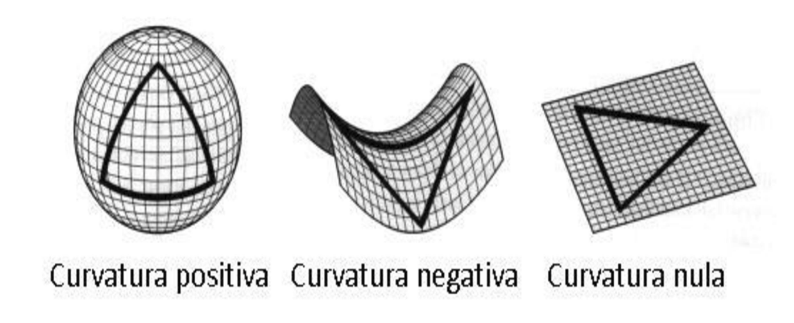
\includegraphics[scale=.4]{./figures/2_theoretical_framework/curvatura_k.png}
\figcaption[Tres espacios con curvatura constante]{\emph{Tres espacios con curvatura constante, esfera con curvatura positiva (izquierda), hiperboloide con curvatura negativa (centro) y plano con curvatura cero (derecha). \scriptsize{\url{https://bit.ly/2Moqlnr}}. }}
\label{fig:curvatura_k}

%--------------------------------------------

Extendiendo el diferencial de linea a tres dimensiones en termino de las coordenadas polar esférica $(\rho, \theta, \phi)$ se llega a 

\begin{equation}
dl^{2}=d\rho^{2}+R^{2}_{c}\sin^{2}\left(\frac{\rho}{R_{c}}\right)[d\theta^{2}+\sin^{2}\theta d\phi]\,,
\end{equation}
%
y como se hizo anteriormente también se puede llegar a la ecuación en términos de $x, \theta, \phi$

\begin{equation}
dl^{2}=\frac{x^{2}}{1-kx^{2}}+ x^{2}[d\theta^{2}+\sin^{2}\theta d\phi]\,.
\end{equation}
%
Ahora se puede proceder a escribir la métrica considerando el tiempo y llegar a una métrica espacio-temporal   

\begin{equation}
ds^{2}=dt^{2}-\frac{1}{c^{2}}dl^{2}\,.
\label{ec:metrica_general}
\end{equation}

Para un modelo del universo isotrópico, se tiene una función que permite describir como cambia la escala espacial entre dos observadores cualesquiera en un instante de tiempo $t$. $a(t)$ es conocido como el factor de escala y viene dada por 

\begin{equation}
\rho(t)=a(t)r\,,
\end{equation} 
%
$r$ es llamada la \textit{ coordenada radial de distancia comóvil}. Se establece que $a(t)=1$ si $t=t_{o}$ que equivale al universo de hoy.\\

Llamando $\Re$ como el radio de curvatura para la presente época ($R_{c}(t_o)$), se obtiene  que el radio de curvatura es: 

\begin{equation}
R_{c}=a(t)\Re \,.
\end{equation}
%
Sustituyendo $\rho$ y $R_{c}$ en la métrica (\ref{ec:metrica_general}) y considerando el diferencial de ángulo solido $d\Omega^{2}=d\theta^{2}+\sin^{2}\theta d\phi^{2}$ se obtiene 

\begin{equation}
ds^{2}=dt^{2}-\frac{a^{2}(t)}{c^{2}}[dr^{2}+\Re^{2}\sin^{2}(r/\Re)d\Omega^{2}]\,.
\end{equation}
%
Esta es la métrica de Robertson-Walker. Es importante notar que $a(t)$ indica como cambia el espacio donde evoluciona el Universo y $\Re$ describe la curvatura espacial del Universo en la presente época.

Otra forma de representar la métrica es usando \textit{diametro angular comóvil} $r_{1}=\Re\sin(r/\Re)$

\begin{equation}
ds^{2}=dt^{2}-\frac{a^{2}(t)}{c^{2}}\left[\frac{dr^{2}_{1}}{1-kr^{2}_{1}}+r^{2}_{1}d\Omega^{2}\right]\,,
\end{equation}
%
donde $k=1/\Re^{2}$.

Retomando la ecuación inicial (\ref{eq:tensor_metrico}), el tensor métrico $g_{\mu\nu}$ sería


%\begin{bmatrix}
%1 & 0 & 0 & 0\\ 
%0 & $\frac{-a^{2}(t)}{1-kr^{2}}}$ & 0  & 0\\ 
%0 & 0 & $-a^{2}(t)^{2} $  & 0 \\ 
%0 & 0 & 0 & $-a^{2}(t)\sin^{2}(\theta)$
%\end{bmatrix}


\begin{equation}
g_{\mu\nu}=
\begin{bmatrix}
1 & 0 & 0 & 0 \\ 
0 & \frac{-a^{2}(t)}{1-kr^{2}} & 0 & 0 \\ 
0 & 0 & -a^{2}(t)  & 0 \\ 
0 & 0 & 0 & -a^{2}(t)\sin^{2}(\theta)
\end{bmatrix}\,.
\label{eq: Metrica}
\end{equation}

Usando la métrica (\ref{eq: Metrica}) y las ecuaciones de campo de Einstein es posible diseñar un modelo del Universo, modelo que puede ser construido a partir de las ecuaciones de Friedmann. 



%\newpage
%*************************************************************************
%The Friedmann equations
\subsection{Ecuaciones de Friedmann}
\label{subsec:Ecuaciones_Friedmann}
%************************************************************************

En Relatividad General, las ecuaciones de campo de Einstein brindan información muy importante sobre la relación entre la energía, masa y la geometría del espacio-tiempo, cuya relación es dada por 

\begin{equation}
R_{\mu\nu}-\frac{1}{2}R-g_{\mu\nu}\Lambda=\frac{8\pi G}{c^{4}}T_{\mu\nu} \,,
\label{eq:Einstein_campo_ecuacion}
\end{equation}
%
donde $R_{\mu\nu}$ es el tensor de Ricci, $R$ es el escalar de Ricci, $g_{\mu\nu}$ es la métrica, $\Lambda$ constante cosmológica y $T_{\mu\nu}$ es el tensor momentum-energía. 

El tensor y escalar de Ricci se pueden calcular como 

\begin{eqnarray}
R_{\mu\nu} \equiv \partial_{\lambda}\Gamma^{\lambda}_{\mu\nu} - \partial_{\nu}\Gamma^{\lambda}_{\mu\lambda} + \Gamma^{\lambda}_{\lambda\rho} \Gamma^{\rho}_{\mu\nu} - \Gamma^{\rho}_{\mu\lambda} \Gamma^{\lambda}_{\nu\rho}\,,
\end{eqnarray}

\begin{equation}
R=R^{\mu}\,_{\mu}=g^{\mu\nu}R_{\mu\nu}\,,
\label{eq:Tensor_Ricci}
\end{equation}
%
donde 

\begin{equation}
\Gamma^{\nu} \,_{\alpha\beta}=\frac{1}{2}g^{\mu\sigma}(\partial_{\beta} g_{\sigma\alpha}+\partial_{\alpha} g_{\sigma\beta}-\partial_{\sigma} g_{\alpha\beta})\,.
\end{equation}

Debido a la isotropía del espacio en la métrica de \textit{Robertson-Walker}, no es necesario calcular las componentes $R_{i0}=R_{oi}$. Las componentes que no se hacen cero del tensor de Ricci son


\begin{eqnarray}
R_{00}=-3\frac{\ddot{a}}{a}\,, \hspace{2cm} \\
R_{ij}=-\left[\frac{\ddot{a}}{a}+ 2\left(\frac{\dot{a}}{a}\right)^{2} + 2\frac{k}{a^{2}} \right]g_{ij} \hspace{1cm} i,j=0,1,2\,,
\end{eqnarray}

\begin{align}
R_{\mu\nu}=R_{00}+R_{ij}\,,
\label{eq: tensor_Ricci}
\end{align}

y el escalar de Ricci queda 

\begin{equation}
R=-6\left[\frac{\ddot{a}}{a} + \left(\frac{\dot{a}}{a} \right) + \frac{k}{a^{2}} \right]\,.
\label{eq:Ricci_escalar}
\end{equation}

En cosmología cuando se pretende calcular el tensor momentum-energía, se considera  un fluido perfecto. Tomando el tensor como la suma de sus componentes $T_{\mu\nu}=T_{ij}+T_{i0}+T_{0j}+T_{00}$, y debido a la isotropía se tiene que $T_{i0}=T_{0j}=0$. Al considerar entonces la isotropía y la homogeneidad se tiene

\begin{equation}
T_{00}= \rho(t)\,, \hspace{1cm} T_{io}=0\,, \hspace{1cm} T_{ij}=-P(t)g_{ij}(t,\bf{x})\,.
\label{eq: Tensor_momentum-energia}
\end{equation}
%
Remplazando (\ref{eq: Tensor_momentum-energia}), (\ref{eq:Ricci_escalar}) y (\ref{eq: tensor_Ricci}) en la ecuación (\ref{eq:Einstein_campo_ecuacion}), se llega a dos ecuaciones escalares acopladas

\begin{equation}
\frac{\ddot{a}}{a} = -\frac{4\pi G}{3}\left(\rho + \frac{3P}{c^{2}} \right) + \frac{c^{2}\Lambda}{3}\,,
\end{equation}
\begin{equation}
\frac{\ddot{a}}{a}+2 \left(\frac{\dot{a}}{a}\right)^{2} + 2k\left(\frac{c}{a} \right)^{2} =4\pi G\left( \rho - \frac{P}{c^{2}}\right)+ c^{2}\Lambda\,,
\end{equation}
%
donde $\rho$ es la densidad y $P$ es la presión.

La importancia de estas ecuaciones radica en que permiten conocer la evolución del universo (homogéneo e isótropo) usando el factor de escala. 


%*************************************************************************
%The Friedmann equations
\section{Formación de estructuras}
\label{sec: Estructure_Formation}
%************************************************************************



%Buscando poder demostrar un modelo que permita modelar la estructura del universo a gran escala, se hace uso de la {\it{Inestabilidad de Jeans}}. Esta teoría representa la evolución del universo, partiendo de los principios fundamentales (homogeneidad e isotrpía).

Al observar el universo a gran escala, se evidencia que este posee alta simetría y homogeneidad, pero ?`qué pasa cuando se mira a escalas menores? A escalas menores que la cosmológicas, los sistemas son anisótropos e inhomogéneos, lo cual implica una alta complejidad. Por esto, es necesario realizar modelos que permitan reproducir las observaciones, asumiendo aproximaciones coherentes,  haciendo que el grado de dificultad disminuya. El universo a escalas menores que las cosmológicas, presenta no linealidad en muchos fenómenos físicos; la formación de estructuras es un caso de ello. 
%La forma de introducir la linealidad o no linealidad en la formación de estructuras es considerando el campo de densidad. 
Para él régimen lineal de formación de estructuras se tiene que $\delta\rho << \bar{\rho}$, donde la perturbación de la densidad es mucho menor que la densidad media. Mientras que para el régimen no lineal se supone que la perturbación es aproximada o mayor a la densidad media ($\delta\rho \sim \bar{\rho}$).


Con el propósito de poder reconstruir la estructura del universo en cualquier instante $t$ se considera lo siguiente:

Al observar el pasado, se debe pensar que existieron pequeñas desviaciones en la homogeneidad en el campo de densidad de materia. A medida que el tiempo pasa, estas desviaciones crecen, debido a la fuerza gravitacional. Esto fue generando una acumulación de materia cada vez mayor en regiones donde la sobre densidad y por ende el pozo de potencial gravitacional aumentaban
, esto desencadenó la formación de estructuras, que dio origen a las primeras galaxias. 
%Las soluciones a las ecuaciones de Friedmann permiten incorporar las perturbaciones que darán origen a la formación de las estructuras.

Se debe tener presente que la teoría del régimen lineal solo se cumple para desviaciones pequeñas del campo de densidad, osea, para un universo muy joven o para escalas muy grandes, donde los modos del campo de densidad aun no se han acoplado. Para poder reproducir las estructuras del universo observable, es necesario considerar un teoría de régimen no lineal. Si se desea profundizar más en este tema, se recomienda abordar los libros: \cite{padmanabhan1995}, \cite{longair2008}, \cite{coles2002}. Los cueles fueron los textos de referencia.


%*************************************************************************
%Structure Formation
\subsection{Régimen lineal para la formación de estructuras}
\label{subsec:Lineal_Estructure_Formation}
%************************************************************************


%---------------------------------------------------------------------
	%M
	\subsubsection{Régimen Newtoniano}
	\label{subsubsec:Newtonian_Regimen}
	%---------------------------------------------------------------------


En el régimen lineal la perturbación en la métrica $g_{\mu\nu}$ y su fuente $T_{\mu\nu}$ se escriben de la forma

\begin{equation}
g_{\mu\nu} \Rightarrow g_{\mu\nu}+\delta g_{\mu\nu} \hspace{0.8cm} T_{\mu\nu} \Rightarrow T_{\mu\nu} +\delta T_{\mu\nu} \,.
\end{equation}
%
Al suponer que las perturbaciones son pequeñas es posible linealizar la ecuación de Einstein 

\begin{equation}
\hat{\mathcal{L}}(g_{\mu\nu})\delta g_{\mu\nu} = \delta T_{\mu\nu} \,,
\end{equation}
%
donde $\hat{\mathcal{L}}$ es un operador diferencial lineal que depende del espacio-tiempo. 
 
Una forma simple de poder calcular la dinámica de las perturbaciones es teniendo en cuenta que el radio de la perturbación es menor al radio de Hubble. Al decir esto se puede despreciar los efectos relativistas y poder usar un tratamiento Newtoniano para las perturbaciones. Al suponer esto, se puede considerar la materia del universo como un fluido Newtoniano que colisiona. Esto implica que es posible usar las ecuaciones de un fluido Newtoniano:

\begin{eqnarray}
\frac{\partial \rho}{\partial t} + \nabla\cdotp(\rho v) = 0\,, \hspace{1cm} Ecuacion\ de\ continuidad \\
\label{eq: Navier-Stoke1}
\frac{\partial v}{\partial t} +(v\cdot \nabla)v = -\frac{\nabla p}{\rho}- \nabla\Phi \,,  \hspace{0.5cm} Ecuacion\ de\ Euler\\
\label{eq: Navier-Stoke2}
\nabla^{2}\Phi = 4\pi G\rho\,. \hspace{1.3cm} Ecuacion\ de\ Poisson\\
\label{eq: Navier-Stoke3}
\end{eqnarray}

Al aplicar las pequeñas perturbaciones cuasiestáticas a la densidad ($\rho=\rho_{o}+\delta\rho$), velocidad ($v=\delta v$), presión ($p=p_{o}+\delta p$) y al potencial gravitacional ($\Phi=\Phi_{o}+\delta\Phi$). Se obtiene 

%\begin{subequations}
\begin{align}
\frac{\partial \delta\rho}{\partial t} + \rho_{o}\nabla\cdotp(\delta v) = 0\,,
\label{eq:Navier-stoke1_perturbation}
\end{align}
%----------------
\begin{align}
\frac{\partial \delta v}{\partial t} + \frac{1}{\rho}\left(\frac{\partial p}{\partial \rho} \right)\nabla \delta \rho+ \nabla\delta\Phi =0\,,
\label{eq:Navier-stoke2_perturbation}
\end{align}
%-------
\begin{align}
\nabla^{2}\delta\Phi - 4\pi G\delta\rho = 0\,.
\label{eq:Navier-stoke3_perturbation}
\end{align}	
%\end{subequations}

Ahora el propósito es poder resolver las ecuaciones con perturbaciones (\ref{eq:Navier-stoke1_perturbation}, \ref{eq:Navier-stoke2_perturbation}, \ref{eq:Navier-stoke3_perturbation}). 
La combinación de estas ecuaciones conducen a la ecuación de la perturbación que se parece a la una ecuación de onda plana. Para resolverla
se puede suponer soluciones de ondas planas\footnote{Cuando se supone un universo plano, se consideró la aparición de las ondas planas}

\begin{equation}
\delta u_{i} = \delta_{i}e^{i\bf{k}\cdot \bf{r}}\,,
\end{equation}
%
donde $\delta u_{i}= \delta\rho, \delta v, \delta\Phi$ y se entiende que $\delta_{i}$ equivale a las amplitudes. 
%%Mi propósito no es solucionar estas ecuaciones, solo pretendo mostrar que consideraciones se deben hacer para llegar a los resultados
~\\

Al considerar la inestabilidad gravitacional propuesta por Jeans, se puede obtener unos resultados  interesantes sobre la formación de la estructura:
%. Entonces considerando lo siguiente: 

Para un fluido homogéneo e isotrópico, se tiene que a medida que el sistema evoluciona se van generando pequeños cambios en la densidad $\delta \rho$ y en la velocidad $\delta v$.

De igual manera se plantea que la aparición de una inhomogeneidad en la distribución de materia $\delta\rho$  generará un cambio en la fuerzas que preservan la homogeneidad. Entonces si $\delta\rho>0 $  la fuerza de gravitación $F_{g}$ responsable del colapso, deberá ser mayor que la fuerza de presión $F_{p}$(responsable del no colapso), entonces   $F_{g}>F_{p}$. Esta ultima afirmación da la condición necesaria para la formación de estructuras. Usando esta idea se puede determinar el radio necesario para el cuál se cumple la desigualdad, también conocido como el radio de Jeans $\lambda$.  

\begin{eqnarray}
F_{g} \approx G\rho\lambda \ \ \  y \ \ \ F_{p}\approx\frac{v_{s}^{2}}{\lambda}\\
\lambda^{2} > \frac{v_{s}^{2}}{G\rho} \,,
\end{eqnarray}

de una forma similar se puede llegar al tiempo gravitacional de caída libre 

\begin{equation}
\tau_{f-f} \approx \frac{1}{(G\rho)^{1/2}}\,.
\end{equation}


%*************************************************************************
%The Friedmann equations
\subsection{Régimen no lineal para la formación de estructuras}
\label{subsec:non-Lineal_Estructure_Formation}
%************************************************************************

Cuando se observa el universo en sus etapas tempranas, antes de la era de la recombinación\footnote{Instante en el universo donde la temperatura bajo lo suficiente para poder permitir la combinación de los electrones con los núcleos generando los primeros átomos. Antes de este instante se conoce como la época dominada por la radiación, electrones y protones libres.}, se considera que las fluctuaciones $\delta$  en la materia eran despreciables ($\delta \ll 1$). La anterior aproximación solo permite resolver el régimen lineal, por ende no funciona al querer describir el Universo actual a escalas galácticas, donde se manifiesta una alta no linealidad.  Sin embargo, si se pretende determinar la evolución dinámica y de las estructuras del Universo a escalas mayores como en la actualidad, donde $\delta \gg 1$, es necesario hacer uso de otro método o aproximación que permita reconstruir la dinámica del universo. 
%Para ello se hace uso del régimen no lineal. 
Cabe resaltar que estos métodos o aproximaciones son altamente complicados 
%donde es necesario hacer aproximaciones 
y muchas veces no es posible llegar a soluciones analíticas, por esto se hace uso de los métodos numéricos que permiten encontrar aproximaciones a las soluciones. 

Una forma de poder aproximar el comportamiento del régimen no lineal que presenta el Universo actualmente, es considerando la aproximación de Zeldovich, la cual provee una descripción apropiada del régimen quasi-lineal. 

%En la actualidad existe una gran variedad de métodos que describen la formación no lineal. Un caso especial es la aproximación de Zeldovich, la cual es capaz de reproducir el régimen lineal, permitiendo usar una  expresión analítica y reduciendo la complejidad de los cálculos. Este método además reproduce de muy buena manera el universo observable actual.

%-----------------------------------------
%\includegraphics[scale=.4]{./figures/2_theoretical_framework/Zeldovich.gif}
%\figcaption{\emph{Tres espacios con curvatura constante, esfera con curvatura positiva (izquierda), hiperboloide con curvatura negativa (centro) y plano con curvatura cero (derecha)}.}\label{fig:zeldovich_box}

%--------------------------------------------


%---------------------------------------------------------------------
	%M
	\subsubsection{Aproximación de Zeldovich}
	\label{subsubsec:Zeldovich_Aproximation}
	%---------------------------------------------------------------------

Bajo el régimen no lineal, es posible llegar a resultados importantes de una forma analítica, asumiendo ciertas aproximaciones. Un caso particular es la aproximación de Zeldovich, que además de presentar unos resultados muy congruentes con las observaciones, permite llegar a ellos de forma analítica. 

Es posible usar la aproximación de Zeldovich si se supone que las escalas de la perturbación son menores que la distancia $d_{H}$ (radio de Hubble), lo cual permite hacer un análisis Newtoniano. La aproximación Zeldovich además comienza con suponer un universo homogéneo, con densidad uniforme $\rho_{b}(t)$, el  cual presenta pequeños crecimientos en las perturbaciones. Considerando la posición de cada porción del fluido $\bf{r}(t)$ en coordenadas Lagrangianas y relacionadas con la posición inicial $\bf{q}$

\begin{align}
{\bf{r}}(t)=a(t){\bf{q}}\,.
\end{align}

Bajo la aproximación lineal, lo necesario para poder reproducir un crecimiento en las perturbaciones es adicionar una función separable dependiente de $t$ y $\bf{q}$, $f(t){\bf{p}}({\bf{q}})=a(t)b(t){\bf{p}(\bf{q})}$, que se puede representar de la forma 
%
\begin{align}
{\bf{r}}(t)=a(t){\bf{x}}(t)=a(t)[{\bf{q}}+b(t){\bf{p(q)}}]
\label{eq:Linear_pertubation}
\end{align}
%
donde ${\bf{x}}$ representa la coordenada comovil, $a(t){\bf{q}}$  la expansión cosmológica y $b(t){\bf{p(q)}}$ la perturbación. Se sabe además que $b(t)$ describe la evolución de la perturbación en el régimen lineal. Por tanto la ecuación (\ref{eq:Linear_pertubation}) es capaz de describir la evolución lineal.

Para poder demostrar que la ecuación (\ref{eq:Linear_pertubation})  evoluciona linealmente, es necesario poder conocer cómo evolucionan las perturbaciones de la densidad de cada porción del fluido, bajo el régimen de la ecuación (\ref{eq:Linear_pertubation}). Al considerar $\bar{\rho}$ como la densidad inicial sin perturbación, por conservación de la masa se obtiene lo siguiente

\begin{align}
\underbrace{\rho({\bf{r}},t)d^{3}{\bf{r}}}_{{\textsl{Masa\ en\ cualquier\ instante}}} = \underbrace{\bar{\rho}d^{3}{\bf{q}}}_{{\textsl{Masa\  inicial}}} \,.
\end{align}
%
Por lo tanto

\begin{align}
\rho({\bf{r}},t) = \bar{\rho}\det(\partial q_{i}/\partial r_{j})=\frac{\bar{\rho}/a^{3}}{\det(\partial x_{j}/\partial q_{i})} = \frac{\rho_{b}(t)}{\det(\delta_{ij} + b(t)(\partial p_{j}/ \partial q_{i}))}\,,
\label{eq:density}
\end{align}
%
donde $\rho_{b}(t)=\bar{\rho}/a^{3}(t)$. Calculando el Jacobiano de primer orden de la perturbación

\begin{align}
\frac{\delta\rho}{\rho}=\frac{(\rho-\rho_{b})}{\rho_{b}} = -b(t)\bf{\nabla_{q}\cdot p }\,.
\label{eq:Underdensity}
\end{align}
%
Cuando se observa la solución de la teoría lineal se tiene 

\begin{align}
\frac{\delta\rho}{\rho}=g(t)=\sum_{k}{\bf{A_{k}}}\exp(i{\bf{k}}\cdot[{\bf{q}}+b(t_{i}){\bf{p(q)}}])\,,
\end{align}
%
donde $g(t)$ describe la evolución del contraste de densidad, y ${\bf{A_{k}}}$ es la transformada de Fourier del contraste de densidad inicial. Para un tiempo inicial se tiene que $b(t){\bf{p}}\ll {\bf{q}}$, entonces

\begin{align}
{\bf{p(q)}}=\sum_{k}\frac{i{\bf{k}}}{k^{2}}{\bf{A_{k}}}\exp(i{\bf{k\cdot q}})\,.
\end{align}

Esta ultima ecuación implica que la ecuación (\ref{eq:Linear_pertubation}) sí es capaz de reproducir el régimen lineal. De igual manera, usando el resultado anterior es posible escribir ${\bf{p(q)}}$ de la forma

\begin{align}
{\bf{p(q)}} = \nabla_{q}\Phi_{0}(q), 
\end{align}
%
donde 

\begin{align}
\Phi_{0}(q) = \sum_{k}\frac{{\bf{A_{k}}}\exp(i{\bf{k\cdot q}})}{k^{2}}\,.
\end{align}

Usando una de las ecuaciones de Friedmann $\ddot{a}=-(4\pi G\rho_{b}a)/3$ es posible escribir la ecuación

\begin{align}
\nabla_{q}^{2}\Phi_{0}=\frac{4\pi Ga^{2}(\rho-\rho_{b})}{3ab\ddot{a}}\,.
\end{align}
%
Con ello se obtiene la forma del potencial gravitacional perturbado

\begin{align}
\nabla_{x}^{2}\phi=4\pi Ga^{2}(\rho-\rho_{b})\,,
\end{align} 
%
donde $\phi = 3a\ddot{a}\Phi_{0}$.  Entonces $\Phi_{0}$ es proporcional al potencial gravitacional de la teoría lineal y ${\bf{p(q)}}$ es proporcional al campo de velocidad peculiar de la teoría lineal. 

Por lo tanto, ${\bf{p(q)}}$ es un gradiente de una función escalar, y el Jacobiano de la ecuación (\ref{eq:density}) da como resultado una matriz simétrica; la cual puede ser diagonalizada en cada punto $\bf{q}$, para producir un conjunto de autovalores $-\lambda_{i}(q)$. Ahora, si los autovalores del Jacobiano ($\partial p_{i}/\partial q_{i}$) son de la forma $[-\lambda_{1}({\bf{q}}),-\lambda_{2}({\bf{q}}),-\lambda_{3}({\bf{q}})]$ entonces la densidad de perturbación está dada por 

\begin{align}
\rho({\bf{r}},t)=\frac{\rho_{b}(t)}{(1-b(t)\lambda_{1}({\bf{q}}))(1-b(t)\lambda_{2}({\bf{q}}))(1-b(t)\lambda_{3}({\bf{q}}))}\,.
\end{align}
%
Esta ecuación representa los cambios producidos por la deformación de un cubo infinitesimal, siendo consecuente con los cambios en la densidad. A medida que aumenta la perturbación, la función $b(t)$ también cambia con el tiempo; además el signo de los autovalores proporcionan información de la dinámica del sistema: Cuando se tiene que $\lambda_{i}>0$, el autovalor va en dirección contraría al gradiente del campo de densidad, entonces colapsa. Mientras que si $\lambda_{i}<0$, el autovalor va en la misma dirección del gradiente del campo de densidad, conllevando una expansión. Donde el gradiente del campo de densidad tiene la dirección del autovector $e_{i}$. Los autovalores se pueden diferenciar uno del otro, de la forma $\lambda_{1}\geq \lambda_{2}\geq \lambda_{3}$. El valor particular de cada autovalor $\lambda_{i}$, proporciona información de la dinámica (colapso o expansión) de la materia en ciertas regiones del espacio, dando un criterio para la clasificación de las estructuras.  

\begin{center}
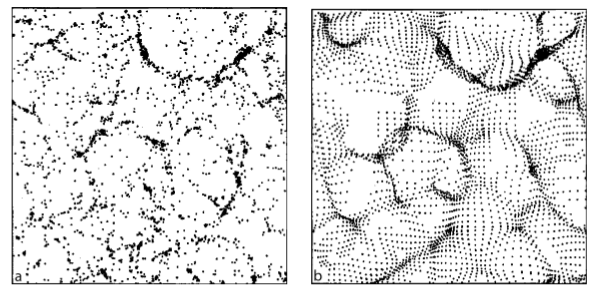
\includegraphics[scale=.5]{./figures/2_theoretical_framework/N-body_Vs_Zeldovich_appro.png}
\figcaption[Comparación entre el modelo de N-cuerpos (a) y la aproximación de Zeldovich]{\emph{Comparación entre el modelo de N-cuerpos (a) y la aproximación de Zeldovich \cite{coles2002}, para las mismas condiciones iniciales; Dejando ver la alta similitud y la buena aproximación del método de Zeldovich en el régimen no lineal. }}\label{fig:diferencial_linea_esferico}
\end{center}






%*************************************************************************	
%qqqqqqqqqqqqqqqqqqqqqqqqqqqqqqqqqqqqqqqqqqqqqqqqqqqqqqqqqqqqqqqqqqqqqqqqq
%Quote
\begin{savequote}[50mm]
%‘‘El cosmos es todo lo que es, todo lo que fue y todo lo que será. Nuestras 
%más ligeras contemplaciones del cosmos nos hacen estremecer: Sentimos como 
%un cosquilleo nos llena los nervios, una voz muda, una ligera sensación como
%de un recuerdo lejano o como si cayéramos desde gran altura. Sabemos que nos
%aproximamos al más grande de los misterios.’’
%\qauthor{Carl Sagan}
\end{savequote}
%qqqqqqqqqqqqqqqqqqqqqqqqqqqqqqqqqqqqqqqqqqqqqqqqqqqqqqqqqqqqqqqqqqqqqqqqq




%#########################################################################
\chapter{Teoría sobre AGN.}
\label{cha:Theoretical Framework}


Al observa la luz de las galaxias en el óptico e infrarrojo cercano, se ve que es dominado mayormente por estrellas, con una pequeña contribución de polvo y gas. Partiendo del hecho de que el espectro de las estrellas puede ser considerado como un espectro de Plank, el cual depende de la temperatura, la masa y edad estelar. Entonces es posible considerar el espectro de una galaxia como la superposición de espectros  estelares. Bajo esta aproximación se puede además decir, que el espectro de las galaxias sería la superposición de espectros de Plank, definidos en un rango de temperaturas. 

Sin embargo, algunas galaxias presentan anomalías en sus espectros,  mostrando una distribución de energía mucho mayor. Algunas enseñan líneas de emisión en zonas poco comunes, y otras en rangos muy amplios, desde las longitudes de onda del radio hasta rayos-X, y algunas hasta rayos gamma. Ver figura (\ref{fig:Espectro_QSOs}). Estas emisiones se originan en regiones muy centrales de la galaxia, por lo cual se les dio el nombre de Núcleo Activo de Galaxias (AGN's por sus siglas en ingles).

Se considera que el causante de la activación de los AGNs son las interacciones gravitacionales. La interacción debida a la fuerzas de marea o la fusión de galaxias genera una turbulencia en el potencial gravitacional que provoca que el gas empiece a colapsar hacia el centro de la galaxia. 

En la actualidad existe una distinción para los diferentes tipos de  AGN's, un tipo específico son los cuásares. Son objetos muy luminosos, su brillo puede superar por un factor de cien el brillo de su galaxia anfitriona. Los procesos que ocurren al interior de un AGN son los más energéticos en el ámbito de la astrofísica. 


%*************************************************************************
%Introducción a AGN's
\section{Introducción a AGN's}
\label{sec:Introduction_AGN's}
%***********************************************************************

Los AGNs son considerados los motores centrales de las galaxias. Su  actividad nuclear esta patrocinada por la acreción de materia. 

Si se desea profundizar más en la teoría de los AGN's, se recomienda abordar los textos: \cite{schneider2006} y \cite{carroll2007}. Estos fueron los textos en que se baso este capítulo. 


%---------------------------------------------------------------------
	%historia
	\subsection{Historia}
	\label{subsec:History}
%---------------------------------------------------------------------
	
En la época de 1908, se observó que la galaxia NGC 1086 que presentaba fuertes lineas de emisión, que eran poco comunes. En 1943, Carl Seyfert a través de un análisis sistemático pudo identificar una nueva clase de galaxia, las cuales llevan su nombre. Estos núcleos de galaxias activas (Seyferts) presentan un muy alto brillo superficial, y su espectro en la región central esta dominado por fuertes líneas de emisión y de alta extinción.  

Los catálogos 3C y 3CR (Catálogos en infrarrojo). \footnote{Catálogo de observaciones hechas con el Cambridge four-element interferometer a una frecuencia de 159MHz} permitieron encontraron objetos muy puntuales con una muy alta línea de emisión. Esta alta emisión no permitía determinar la forma del objeto central que hospedaba la galaxia. Solo fue cuando se pudieron construir telescopios con un poder de resolución mayor que se pudo ratificar que eran fuentes puntuales. A medida que fue pasando el tiempo y se mejoraron  las observaciones, se empezaron a encontrar más fuentes con estas características. A estos cuerpos se les denomino  Cuásares\footnote{Cuásar viene del ingles Quasars (quasi-stellar radio source)}.

Los cuásares son un tipo específico de AGNs. Sin embargo, una buena forma de conocer las propiedades y arquetipos de  AGN's, es identificando las propiedades de los cuásares. Es por esto que a continuación se presenta una clasificación sobre los diferentes cuásares.  La figura (\ref{fig:Espectro_QSOs}) presenta un espectro típico de AGN, cabe resaltar que dicha imagen es la superposición de espectros de QSOs

\begin{center}
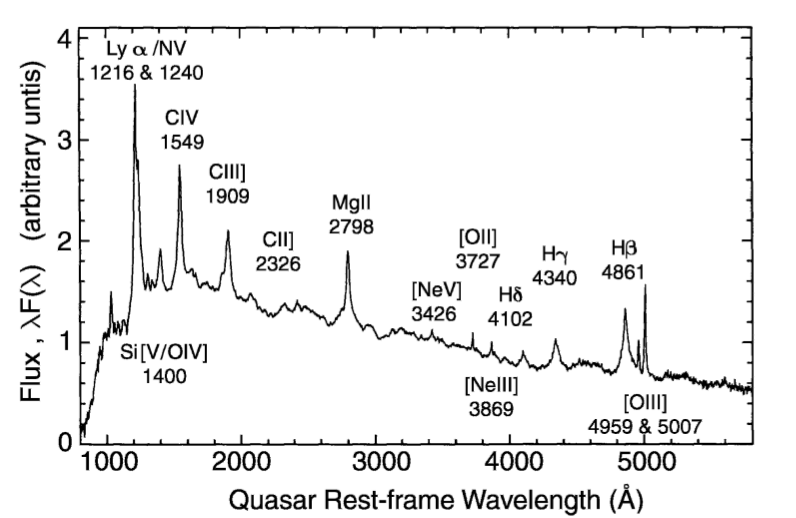
\includegraphics[scale=.3]{./figures/3_AGNs/Espectro_tipico_AGN.png}
\figcaption{\emph{Espectro combinado de varios QSOs, usando las observaciones del Large Bright Quasar Survey \cite{francis1991}.}}\label{fig:Espectro_QSOs}
\end{center}
%---------------------------------------------------------------------
	%M
	\subsection{Propiedades fundamentales de los Cuásares}
	\label{subsec:Fundamental_properties_quasars}
%---------------------------------------------------------------------

Por lo general los cuásares presentan una serie de propiedades que son comunes en varios tipos de AGN's, entre las propiedades se destacan:


- Fueron descubiertos por ser fuentes de radio muy puntual 

- Emite en todas las longitudes de onda, desde el radio a los rayos-X principalmente.

- El flujo de la fuente varía en casi todas las frecuencias y longitudes de onda.

- En general se encuentra que la escala de tiempo de variabilidad es más pequeña y su amplitud más grande, cuando se va ha frecuencias más altas.

- El espectro óptico es muy azul ($U-B < -0.3$). La mayoría de los cuásares presentan un corrimiento a rojo alto  $z \lesssim 2$.

- El espectro continuo de un cuásar puede ser descrito por una ley de potencias, sobre un rango de frecuencias muy alto.
%
\begin{align}
S_{\nu} \propto \nu^{-\alpha} \,,
\end{align}
%
 donde $\alpha$ indica el índice espectral: Cuando $\alpha=0$ entonces se tiene un espectro plano, si $\alpha=1$ se tiene un espectro en el cual la misma energía es emitida en cada intervalo de logarítmico de las frecuencias. 


%---------------------------------------------------------------------
	%M
	\subsection{Cuásares, radio fuentes.}
	\label{subsec:}
%---------------------------------------------------------------------

La morfología de los cuásares en el régimen del radio, depende de la frecuencia observada, que a su vez puede presentar un morfología compleja. La morfología del cuásar en una forma simple se puede ver  constituida por: varias fuentes extendidas y un núcleo central muy compacto, ver figura (\ref{fig:Lobulos}). En algunas ocasiones es posible observar fuentes extendidas llamadas lóbulos, que se extienden de manera casi simétrica a lo largo de una línea recta. Estos lóbulos se encuentra conectados con el núcleo central por cuenta de los jets, que es producto de las partículas cargadas que proveniente del núcleo. El tamaño del sistema en general puede alcanzar hasta 1 Mpc de largo. %La posición óptica coincide con la fuente de radio compacta, cuyo tamaño es mejor a un segundo de arco ($\theta < 1"$).

%---------------------------------------------------------------------
	%
	\subsubsection{Clasificación de las fuentes de radio.}
	\label{subsubsec: clasification_source_radio}
%---------------------------------------------------------------------

Las fuentes de radio extendidas se dividen en dos tipos:

{\it{Fanaroff-Rile Tipo I }} (FR I), son fuentes más brillantes cerca al centro, su brillos superficial decrece hacia el exterior. Poseen una luminosidad típica de $L_{\nu}(1.4GHz)\lesssim 10^{32} erg^{-1} Hz^{-1}$.

{\it{Fanaroff-Rile Tipo II}} (FR II), son fuentes que presentan características contrarias a las (FR I). Su brillo incrementa hacia el exterior, presentando un brillo mayor que las (FR I), $L_{\nu}(1.4GHz)\gtrsim 10^{32} ergs^{-1}Hz^{-1}$, a menudo estas fuentes de radio presentan jets ( Subsección \ref{subsec:Generation_Jets}).

%Los jets, son estructuras que transportan material (partículas cargadas) del núcleo al exterior. Por lo general no son simétricos y a menudo solo es posible ver uno, cuando es posible observar los dos, hay uno más débil que el otro. 


%---------------------------------------------------------------------
	%
	\subsubsection{Radiación Sincrotrón}
	\label{subsubsec: Radiation_synchrotron}
%---------------------------------------------------------------------

La forma espectral y el alto grado de polarización son considerados como consecuencias de la emisión de radio, producida por la radiación sincrotrón\footnote{Radiación producida al someter a partículas cargadas a velocidades muy altas (cercanas a la velocidad de la luz) } de electrones relativistas. Dicha radiación es entonces, el producto de electrones que se propagan a través de un campo magnético, a lo largo de un helicoide, produciendo una fuerza de Lorentz, que los lanza en dirección perpendicular al campo magnético. 

El grado de polarización de un conjunto de electrones depende de la complejidad del campo magnético. Si el campo es homogéneo la medida de polarización observada puede ser mayor al $75\%$. La radiación sincrotrón sigue una ley de potencias, si y solo si  la distribución de energía de los electrones también se comportan como una ley de potencias. 


%*************************************************************************
%AGN Zoo
\section{Tipos de AGN's}
\label{sec:Zoo_AGN's}
%***********************************************************************

Se debe tener muy claro que la diferencia entre los AGN's no radica necesariamente en su forma física. En el contexto de poder "unificar"  los AGN's, su distinción esta altamente relacionado con la dirección de la linea visual, entre la fuente (AGN) y el observador (Telescopio). Ver figura (\ref{fig:Tipos_AGNs_por_observador}).


%---------------------------------------------------------------------
	%M
	\subsection{Quasi-Stelar Objects.}
	\label{subsec:Quasi-Stelar_Objects}
%---------------------------------------------------------------------

Una pequeña cantidad de cuásares presentan un inusual color azul. La presencia de estos objetos en regiones fuera del rango del radio presenta un gran problema para poderlos observar, y siendo además fuentes muy puntuales.

Las propiedades ópticas de estos objetos son casi indistinguibles de los cuásares. En particular, tienen distribución de energías hacia el azul, resultado de la forma de búsqueda; además presentan fuertes y anchas líneas de emisión y en general un alto corrimiento al rojo. Por sus propiedades tan parecidas a los cuásares son llamados como {\textit{radio-quiet quasars ó quasi-stelar objects}}, QSOs. Los QSOs son los AGNs que mayor luminosidad, la cual puede ser 1000 veces más que la luminosidad de la galaxia donde se hospeda.

%---------------------------------------------------------------------
	%M
	\subsection{Galaxias Seyfert.}
	\label{subsec:Seyfert_Galaxy}
%---------------------------------------------------------------------

Como se discutió anteriormente las galaxias Seyferts fueron los primeros AGNs descubiertos. La luminosidad de las Seyferts es considerablemente menor que la de los QSOs. Las observaciones en el óptico permiten identificar que las Seyferts son objetos que se encuentra en el centro de las galaxias espirales, presentando un núcleo extraordinariamente brillante, con líneas de emisión  fuertes y anchas.

Se conocen dos tipos de galaxia Seyfert, las Tipo 1 y las Tipo 2: Las Tipo 1 presentan líneas de emisión muy anchas, lo que supone velocidades de rotación mayor. Las Tipo 2 presentan líneas de emisión más estrechas. Al observar el espectro en el óptico en las Seyfert 1 se identifica que son muy similares a los QSOs. No se conoce una diferencia física entre estos dos objetos, la única diferencia es debida a la luminosidad en sus núcleo. 


%---------------------------------------------------------------------
	%M
	\subsection{Radio Galaxias}
	\label{subsec:Radio_Galaxy}
%---------------------------------------------------------------------

Las radio galaxias son galaxias elípticas que tienen como huésped un AGN. Entre las radio galaxias más conocidas se encuentran Cygnus A y Centuarius A. Al igual que se hizo con las galaxias Seyferts, las radio galaxias también presentan una clasificación debida al ancho de sus  líneas de emisión. Están las radio galaxias de línea ancha (BLRG) y las radio galaxias se línea estrecha (NLRG).

En general los dos tipos de radio galaxias se pueden considerar como radio fuerte Seifert 1 y Seyfert 2, la única diferencia entre Seyfert y radio galaxia es la morfología de la galaxia donde estás hospedadas. 

%---------------------------------------------------------------------
	%M
	\subsection{Variables Opticamente Violentas}
	\label{subsec:Optically_Violently_Variables}
%---------------------------------------------------------------------

Existe otra clase de QSOs, que están caracterizados por su fuerte y rápida variabilidad en su radiación óptica. Son conocidas como OVVs \footnote{Del ingles Optically Violently Variables } (Variables Ópticas Violentas). Estos objetos presentan una variabilidad en escala de tiempo de días. Además de su alta variabilidad, también presentan una muy alta polarización de la luz óptica y fuertes emisiones en radio. Estas fuentes presentan longitudes de onda fuera del rango óptico, aumentando su radiación, con escalas de tiempo más cortas y amplitudes más grandes, a medida que se mueve a frecuencias más altas.  

%---------------------------------------------------------------------
	%M
	\subsection{Objetos BL Lac}
	\label{subsec:BL_Lac}
%---------------------------------------------------------------------

Los BL Lacs son AGNs con una muy fuerte variabilidad en la radiación, como los OVVs, pero sin fuertes líneas de emisión y absorción, haciendo casi imposible la determinación de su corrimiento al rojo $z$. La luminosidad óptica de algunos BL Lacs varia en varias magnitudes si se observa durante periodos de tiempo muy largos.

Algo notable de vez en cuando es el bajón en la luminosidad, a veces se observan líneas de emisión y luego aparece un BL Lac como un OVV. Por este extraño motivo a los OVVs y BL Lacs se les denomina Blazars. Los Blazars son fuentes de radio, con variabilidad violenta y radiación energéticamente fuerte (radiación $\gamma$).


%Es importante recordar que la diferencia de los tipos de AGN radica en la dirección de observación en la cual se ve el AGN. En general el AGN es el mismo, solo que esta siendo observado en lugares diferentes que presentan características específicas, como se observa en la figura (\ref{fig:Tipos_AGNs_por_observador}). 
\begin{center}
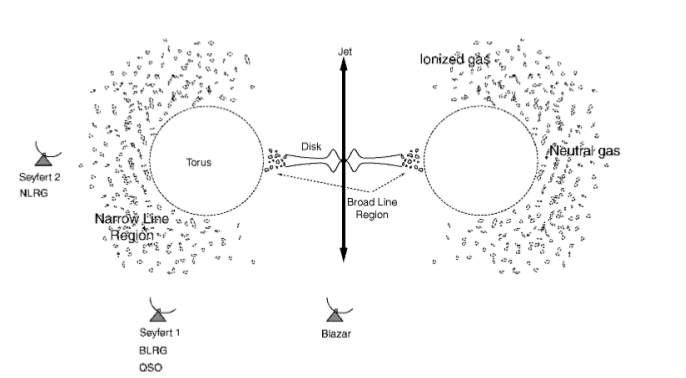
\includegraphics[scale=.5]{./figures/3_AGNs/Clasificacion_AGN}
\figcaption{\emph{Los diferentes tipos de AGNs solo dan información de que lugar del AGN se está observando \cite{schneider2006}.}}\label{fig:Tipos_AGNs_por_observador}
\end{center}


%*************************************************************************
%AGN Zoo
\section{El Enigma Central: La existencia de un Agujero Negro}
\label{sec: Enigma_centarl}
%***********************************************************************

En la teoría de los AGNs, ha existido una duda sobre el proceder de la energía que estos emanan, en especial ?`Cómo es producida? Entonces debido a esto, se plantea que dicha energía es originada por un objeto muy masivo en su interior, muy cercano al centro. El objetos propuesto lleva por nombre  Agujero Negro (BH, Black Hole), presentado como un objeto altamente compacto, que acreta materia de su alrededor. A continuación se presentan una serie de propiedades observacionales en los AGNs que dan pie a la existencia de un BH: \\

- Se encuentran fuentes de radio en AGNs que alcanzan un tamaño aproximadamente mayor a 1 Mpc. Usando esta escala de longitud es posible medir el tiempo en que ha estado activa la fuente. Para esta escala de longitud se tiene que el tiempo de vida es mayor a $10^{7}$años.

-La luminosidad de los QSOs es aproximadamente $L_{bol}\sim 10^{47}ergs$. Asumiendo que la luminosidad no cambia sustancialmente durante el tiempo de vida de la fuente, es posible medir la energía total
\begin{align}
E \gtrsim 10^{47} erg/s \times 10^{7}yr \sim 3\times 10^{61}erg\,.
\end{align}

-Para escalas de tiempo de días, se tiene que la luminosidad de los AGNs varia en un $\% 50$. Estas variabilidades permiten encontrar un límite superior para la extensión espacial de la fuente. Para una fuente puntual se tiene que la extensión es $R \lesssim 1$ día luz $\sim3\times10^{15}$cm.\\

La solución exacta de las ecuaciones de Einsten, predicen la existencia de objetos altamente compacto en cierta región del espacio-tiempo: usando la métrica de {\it{Schwarzschild}} (), se predice la existencia de un Agujero Negro (BH) estático; al usar la métrica de {\it{Kerr}} () se predice la existencia de un BH rotante. 

%---------------------------------------------------------------------
	%M
	\subsection{La Existencia de los Agujeros Negros}
	\label{subsec:Why_a_BH}
%---------------------------------------------------------------------

Usando la información observacional expuesta anteriormente y suponiendo que la producción de energía es de naturaleza gravitacional, es posible derivar la energía básica en el AGN. Suponiendo lo anterior, la forma clásica más eficiente de transformación de energía es por medio de la fusión nuclear. 

La fusión del hidrógeno, produce 8Mev/nucleon. La máxima eficiencia de fusión nuclear es $\epsilon \lesssim 0.81 \%$, donde $\epsilon$ es la fracción de masa del combustible que es convertido en energía. De acuerdo con 
\begin{align}
E=\epsilon mc^{2}\,,
\end{align}
%
la energía por fusión es $E=3\times10^{61}$. Entonces la masa que produce el combustible necesitaría ser 
\begin{align}
m=\frac{E}{\epsilon c^{2}} \sim 4\times10^{42}g\sim 2\times10^{9}M_{\odot}\,.
\end{align}

Al suponer que la naturaleza de la energía es meramente gravitacional, se tiene entonces que a medida que la materia cae dentro del BH pierde energía potencial, pero adquiere energía cinética . Al convertir la energía cinética en energía interna(calor) que será emitida en forma de radiación.

Sin embargo, los BH no son la única solución simple para las ecuaciones de Einstein. La existencia de un SMBH (Supermassive Black Hole) es posible al conocer la naturaleza de la distribución de masa compacta. También se ha encontrado evidencia observacional que ratifica la existencia de estos objetos super masivos. 

%---------------------------------------------------------------------
	%M
	\subsection{Proceso de Acreción.}
	\label{subsec:Acretion}
%---------------------------------------------------------------------

A medida que el gas cae hacia un objeto compacto, las partículas de gas pierden energía potencial que a su vez se convierte en cinética. Al conocer que el momentum angular del gas es finito, se tiene certeza que el gas no puede caer directamente hacia el objeto. A medida que este cae, siente una fricción por la interacción con las otras partículas circundantes, lo que se traduce en una transferencia de momentum, que dará como resultado la formación de un disco de acreción perpendicular al momentum angular. La fricción en el disco será la responsable de desacelerar la velocidad de rotación de las partículas, haciendo que estas caigan hacia el centro y sean acretadas por el BH.  

De acuerdo con el teorema del virial, la mitad de la energía potencial se ha cambiado en energía cinética. Por tanto, la mitad de la energía se ha convertido en energía de rotación. Así, la mitad de la energía potencial se convirtió en energía interna. 

La energía generada por la fricción dinámica en el disco, no cuenta con la suficiente energía para poder escapar de allí, pero aun así es capaz de calentar el gas y producir un engrosamiento en el disco, como en la figura (\ref{fig:Tipos_AGNs_por_observador}).


%---------------------------------------------------------------------
	%M
	\subsection{Generación de Jets.}
	\label{subsec:Generation_Jets}
%---------------------------------------------------------------------

Los lóbulos radiales son producidos por partículas cargadas eyectadas desde el centro del AGN, a velocidades relativistas. Estas partículas son aceleradas desde el núcleo en dos direcciones opuestas. El impulso es producido por la extracción de energía cinética de rotación del BH a través del mecanismo de Blandford- Znajek \cite{blandford1977}. Ver figura (\ref{fig:Modelo_interior_AGN}).% En el disco se encuentra el campo magnético  que está acoplado a este flujo de partículas. 

Al observar un AGN es inevitable ver que los jets producidos son extremadamente delgados y muy rectos. Lo cual implica  que los procesos que lo generaron ocurrieron muy al interior del disco, donde el núcleo es el responsable de colimar estos rayos de alta energía. %Es importante aclarar que este mecanismo no reproduce los flujos de materia relativista; sin embargo hay una nueva rama que pretende dar solución a este problema. La hidrodinámica es la responsable de reproducir los fenómenos con una mayor precisión, pero con el costo de poder computacional.
%
\begin{center}
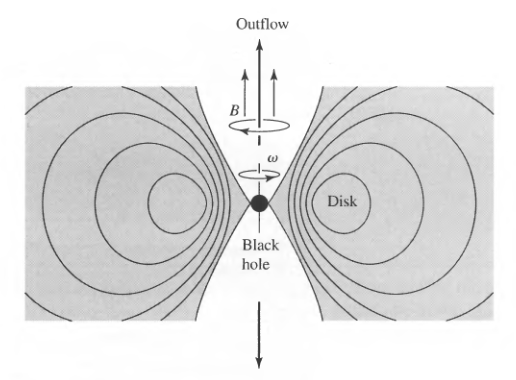
\includegraphics[scale=.5]{./figures/3_AGNs/Jets.png}
\figcaption{\emph{Bosquejo del modelo de la estructura del núcleo del AGN \cite{carroll2007}, donde se puede ver el mecanismo de Blandfort- Znajek}}\label{fig:Modelo_interior_AGN}
\end{center}

%---------------------------------------------------------------------
	%M
	\subsection{Formación de Lóbulos.}
	\label{subsec:Formation_lobules}
%---------------------------------------------------------------------

Cuando los jets expulsan las partículas altamente cargadas del núcleo, estas llevan consigo una energía cinética. A medida que se desplazan por el medio interestelar van perdiendo energía y se van desacelerando. Las partículas que van adelante del flujo de materia, son las que más siente la interacción con otras partículas y se van ralentizando, de una forma más brusca, formando un frente de choque. Este frente de choque provoca que las partículas se vaya esparciendo  de forma desordenada generando los lóbulos, como se observa en la figura (\ref{fig:Lobulos}).

\begin{center}
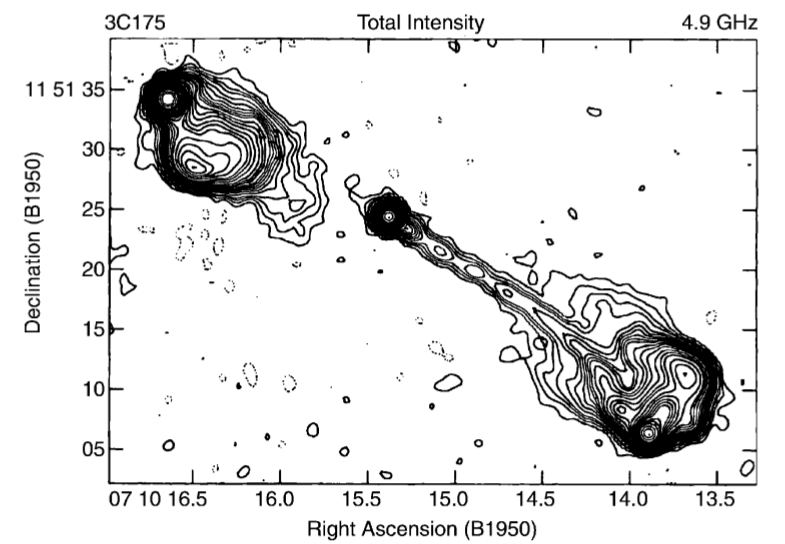
\includegraphics[scale=.3]{./figures/3_AGNs/Lobulos_y_Jets.png}
\figcaption{\emph{Simulación de un AGN\cite{schneider2006}. En la parte central se encuentra el BH, los jets son por donde se desplaza la materia y los lóbulos son los grumos donde se aglomera la materia que viene del núcleo.}}\label{fig:Lobulos}
\end{center}

%*********************************************************************
	%M
\section{Modelo Unificado}
\label{sec:Unified_models}
%*********************************************************************

Conforme a todo lo presentado, se puede identificar que los AGNs presentan cierta similitud, pero de igual manera diferencias considerables. Al conocer su naturaleza, se pretende mostrar a los AGNs como objetos con morfología equivalente, cuya diferencia radica en que son observados en lugares distintos, en los cuales se evidencian fenómenos físicos específicos del AGNs. Mirar figura (\ref{fig:Tipos_AGNs_por_observador}).

Como ya se ha dicho y mostrado los AGNs presentan propiedades en común: \\

- Todas los AGNs hospedan un SMBH en su interior. 

- Todos los AGNs tiene un disco de acreción que alimenta el BH.

- Todos los AGNs van a estar caracterizados por la masa del BH $M_{BH}$ y de la rata de acreción $\dot{m}$. $M_{BH}$ permite relacionar la luminosidad máxima del SMBH. 

- La morfología de la galaxia anfitriona también permite clasificar, como por ejemplo: Las radio galaxias están en galaxias espirales, mientras que las Seyferts en galaxias espirales.\\

Con estos criterios se pretende construir un criterio de clasificación más amplio, que permita albergar todos los tipos de AGNs.





%*************************************************************************
%--------------------------Spin Model ----------------------

%qqqqqqqqqqqqqqqqqqqqqqqqqqqqqqqqqqqqqqqqqqqqqqqqqqqqqqqqqqqqqqqqqqqqqqqqq
%Quote
\begin{savequote}[50mm]
%‘‘El cosmos es todo lo que es, todo lo que fue y todo lo que será. Nuestras 
%más ligeras contemplaciones del cosmos nos hacen estremecer: Sentimos como 
%un cosquilleo nos llena los nervios, una voz muda, una ligera sensación como
%de un recuerdo lejano o como si cayéramos desde gran altura. Sabemos que nos
%aproximamos al más grande de los misterios.’’
%\qauthor{Carl Sagan}
\end{savequote}
%qqqqqqqqqqqqqqqqqqqqqqqqqqqqqqqqqqqqqqqqqqqqqqqqqqqqqqqqqqqqqqqqqqqqqqqqq




%#########################################################################
%*****************************************************
\chapter{Modelo de Espín}
\label{cha:Modelo de Spin}
%*****************************************************

El espín\footnote{El espín hace alusión al momentum angular, para los BHs rotantes se hace uso de la métrica de Kerr.} de BH se sospecha que es un parámetro relevante para la dinámica de las galaxias, se cree que su importancia radica en parte a la dicotomía que existe entre radio loud AGNs y radio quiet AGNs. Este será el responsable de decir si existe alguna relación entre los AGNs y el entorno que habitan. En esta sección se presentarán los modelos que dan pie al origen, evolución y  alineamiento de los espines.

%===============================================
\section{Agujeros Negros Super Masivos (SMBHs)}
\label{sec: SMBH}
%================================================
Los SMBHs son objetos altamente masivos, que presenta un rango de masas entre $10^6M_{\odot}\lesssim M_{BH} \lesssim 10^{9}M_{\odot}$ \cite{mo2010}. Una de las evidencias que sugiere la existencia de los SMBHs, es que serían los causantes de la cantidad de energía que es emitida por los AGNs debido a la acreción de materia (mirar capitulo \ref{sec: Enigma_centarl}). Observaciones en regiones centrales de las galaxias, presentan un incremento en la razón masa-luminosidad, el cual no puede ser explicado por la presencia de poblaciones estelares, indicando que hay una objeto muy masivo, que no presenta una luminosidad considerable, permitiendo postular la existencia de un SMBH, ubicado en la parte central de la galaxia.  

La presencia de un SMBH en la galaxia solo influye dinámicamente en lugares cercanos a él (centrales). Usando la dispersión de las velocidades para estrellas cercanas al centro es posible encontrar un valor para la masa del objeto central, 

\begin{align}
    r_{BH}=\frac{GM_{BH}}{\sigma^{2}}
\end{align}
donde $\sigma$ es la dispersión de la velocidad, obtenida de medidas observacionales. 

En el contexto cosmológico se considera que todas las galaxias hospedan un SMBH en su interior, muy cercano al centro. Su existencia también viene arraigada por la misma teoría, son consecuencia de la relatividad general y de la teoría de formación de galaxias. 

La importancia de los SMBHs radica es su propiedad de acretar materia y convertirla en energía, esta energía liberada se conoce como feedback de agujero negro. Para galaxias grandes, el feedback es el responsable de que la galaxia deje de producir estrellas, debido a que este calienta el gas  impidiendo el colapso gravitacional por parte de las nubes de gas, y por ende impidiendo la formación estelar.

Yendo en dirección de poder conocer la información sobre el espín del BH o SMBH, es necesario saber cómo se originan y evolucionan. Es imperioso por tanto entender la teoría que abarca la evolución y crecimiento de los BHs.
%------------------------------------------------
\subsection{Crecimiento de SMBHs}
\label{subsec: Crecimiento_SMBHs}
%------------------------------------------------

El proceso de crecimiento de un SMBH esta determinado por la rata de acreción de masa. En la actualidad hay tres maneras posibles para el crecimiento del SMBH: fusión de BHs, colapso de nubes frías de gas que está alrededor galaxia y fusión entre galaxias \cite{fanidakis2011}. Cualquiera de estos tres sucesos pueden dar pie a la activación de un AGN, ya que este proceso es producto de la acreción súbita de materia. 
%-------------------------------------------------------
    \subsubsection{Fusión de BHs}
    \label{subsubsec: mergers_BHs}
%-------------------------------------------------------
La adquisición de materia por fusión entre BHs, corresponde a sistemas  binarios. La fricción dinámica que sienten los BHs  hace que estos pierdan momentum angular, dando como resultando una disminución en la separación entre ellos, y posteriormente repercutir en una fusión. También la perdida de energía debido a emisión de las ondas gravitacionales hace que la distancia entre los dos cuerpos se vaya reduciendo. A medida que pasa el tiempo 
la amplitud y por ende la energía de las ondas gravitacionales aumenta a medida que la separación entre los BHs binarios es menor.
%la emisión de las ondas gravitacionales es más consecutiva, haciendo que la perdida de energía sea mayor,
dando como resultado la coalescencia entre los dos BHs \cite{fanidakis2011}. 

%-------------------------------------------------------
    \subsubsection{Colapso de nubes de gas}
    \label{subsubsec: colapso_nubes_gas}
%-------------------------------------------------------
En galaxias de tipo temprano, donde es posible encontrar gas frío que esté en inmediaciones del centro de la galaxia, de tal forma que el gas pueda fluir directamente al BHs. Otra manera de acretar gas frío es por medio del método de radio-mode. Este mecanismo consiste en que el gas que es expulsado y calentado por la explosiones de supernovas o por el mismo SMBH, después de un largo tiempo se enfría y colapsa al centro de la galaxia, donde se encuentra el BH \cite{fanidakis2011}.

%-------------------------------------------------------
    \subsubsection{Colisión de galaxias}
    \label{subsubsec: mergers_galaxys}
%-------------------------------------------------------
La dinámica del universo y las observaciones, dejan ver que la interacción entre galaxias no es en nada extraño, siendo la colisión entre ellas un resultado esperado. Las galaxias espirales en su interior, en especial en la parte más interior del disco presentan una abundancia de gas frio, potencial para: la formación de estrellas, crecimiento de un BH y activación de un AGN. El proceso de fusión entre galaxias se distingue por fusiones mayores y menores\footnote{El proceso de fusión introduce un cambio en la morfología de las galaxias. Si es una fusión menor es posible que no altere la morfología de la galaxia más masiva, de manera considerable, mientras que las fusiones mayores transforma drásticamente la forma de las galaxias. }: las fusiones mayores indican colisiones donde la masa de los dos cuerpos son equivantes (Andromeda y Vía láctea), mientras en las fusiones menores la diferencia entre masas es considerable (Vía láctea y nube de magallanes). Cuando colisionan las dos galaxias, ya sea una fusión mayor o menor, producen un incremento en la formación estelar debido a la acumulación de gas frío de ambas galaxias. Pero no todo el gas frío se transforma en estrellas, parte de este cae al centro alimentando al BH.

%===============================================
\section{Evolución de espín}
\label{sec: Evolution_spin}
%===============================================

La evolución del espín del SMBH está altamente relacionada con la tasa de acreción de materia por parte del SMBH \cite{king2005}, y por la coalescencia de los BHs \cite{dubois2014}. Al considerar el interior de un AGN, se tiene entonces una estructura compuesta por un disco de acreción que orbita alrededor de un SMBH. Al suponer que tanto el SMBH como el disco de acreción rotan, implica un momentum angular (espín) tanto para el SMBH $\bf{J}_{bh}$, como para el disco de acreción $\bf{J}_{d}$. 
Los efectos relativistas producidos por el BH rotante, genera alrededor de él una torsión en el espacio-tiempo (Efecto Lense-Thirring).    
%Los torques de marea 
La torsión que actúan sobre ambos cuerpos rotantes conduce a alinear los espines, sin cambiar sus magnitudes \cite{king2005}.

El espín del SMBH puede ser definido como ${\bf{J}}_{bh}=|a|GM^{2}_{bh}/c$, donde $a$\footnote{normalizazión del momentum angular del BH.} es el parámetro de espín, acotado entre $-1\leq a \leq 1$: Sí $a=-1$ el BH está rotando en dirección contraría al disco de acreción, sí $a=1$ el BH y disco rotan en la misma dirección. ${\bf{J}}_{bh}$ juega un papel crucial para regiones cercanas al BH, indica la eficiencia de convertir la materia del disco en radiación, se cree además que su dirección está relacionada con la dirección del jet de AGN \cite{fanidakis2011}. 

%------------------------------------------------
\subsection{Acreción de gas}
\label{subsec: Acrecion_gas}
%------------------------------------------------
Como se expuso anteriormente, alrededor del SMBH existe un disco de acreción, que es originado por la conservación del momentum angular de una porción de gas  que caen al disco de acreción. Siguiendo lo propuesto por \cite{lynden1969}, las partículas que se encuentran el disco de acreción pierden momentum angular debido a torques producidos por los campos magnéticos, a medida que pierden momentum angular se van adentrando más en el disco, hasta llegar al borde interior del mismo. La orbita más interior es denominada como la ultima orbita estable (del ingles LSO). Sí la partícula se adentra en esta órbita será devorada con seguridad por el BH. El radio para la LSO en términos del momentum angular del BH se puede reescribir de la forma \cite{bardeen1972}:
%
\begin{align}
 \hat{r}_{lso}=\frac{r_{lso}}{R_g}=3+Z_{2}\pm \left[ (3-Z_{1})(3+Z_{1}+2Z_{2})\right]^{1/2} \,,
 \label{eq: radio_lso}
\end{align}
%
donde $R_{g}$ es el radio gravitacional, definido como la mitad del radio de Schwarzchild del BH, 
%
\begin{align}
    R_{g}= R_{schw}/2  = \frac{GM_{bh}}{c}\,.
\end{align}
%
Para valores de $a<0$ se toma el signo positivo de la ecuación (\ref{eq: radio_lso}), indicando que el BH rota de manera contraría al gas que están en la LSO, si $a>0$ se toma el signo negativo de la ecuación (\ref{eq: radio_lso}), obteniendo lo contrario, el BH rota en la misma dirección del gas. Los parámetros $Z_1$ y $Z_2$ se escriben de la forma:
%
\begin{eqnarray}
    Z_1 = 1+(1-a^{2})^{1/3}\left[(1+a)^{1/3}+(1-a)^{1/3} \right]\,,\\
    Z_2 = (3a^{2}+Z_{1}^{2})^{1/2}\,.
\end{eqnarray}
%
Un parámetro de gran importancia es la eficiencia radiativa del disco de acreción del BH $\epsilon_{r}$. Este parámetro indica la fracción de energía liberada por la materia que rota alrededor del BH. Al suponer un BH que rota, la eficiencia radiativa dependerá del parámetro de espín $a$ \cite{novikov1973}:
%
\begin{align}
    \epsilon_{r} \equiv 1- \sqrt{1-\frac{2}{3}\frac{1}{\hat{r}_{lso}(a)}}\,,
    \label{eq: eficiencia radiativa}
\end{align}
%
en otras palabras: entre más acreta menos irradia ó entre más irradia menos acreta.

A medida que el material cae a la LSO y posteriormente al BH, conlleva  una emisión de energía por unidad de masa $\widetilde{e}_{lso}$ y un momentum por unidad de masa $\widetilde{l}_{lso}$. Al considerar la masa contenida en una región muy cerca a LSO $dM_{0}$, permitiendo calcular el cambio de la masa y del momentum angular del BH, de la forma \cite{fanidakis2011}:
%
\begin{align}
    dM_{bh}=\frac{\widetilde{e}_{lso}}{c^{2}}dM_{0}, \, \, dJ_{bh}=\widetilde{l}_{lso}dM_{0}\,.
    \label{eq: dM_y_dJ}
\end{align}
%
La ecuación (\ref{eq: dM_y_dJ}) se relaciona con la ecuación para el espín del BH total ${\bf{J}}_{bh}$ de la forma:
%
\begin{align}
    \frac{da}{d\ln{M_{bh}}}=\frac{1}{M_{bh}}\frac{c^{3}}{G}\frac{\widetilde{l}_{lso}}{\widetilde{e}_{lso}}-2a\,,
\end{align}
%
La integral a esta solución es obtenida por \cite{bardeen1970}, dando como resultado: 
\begin{align}
    a^{f}=\frac{1}{3}\hat{r}_{lso}^{2}\frac{M_{bh}}{M_{bh}^{f}}\left[1- \left\{3\hat{r}_{lso}\left(\frac{M_{bh}}{M^{f}_{bh}} \right)^{2}-2 \right\}^{1/2} \right]\,,
    \label{eq: espin_final a^f}
\end{align}
donde $a^{f}$ y $M_{BH}^{f}$, corresponden al espín y masa final del BH. La ecuación (\ref{eq: espin_final a^f}) determina la evolución del espín $a$ durante el tiempo de acreción para un estado inicial. 

\begin{center}
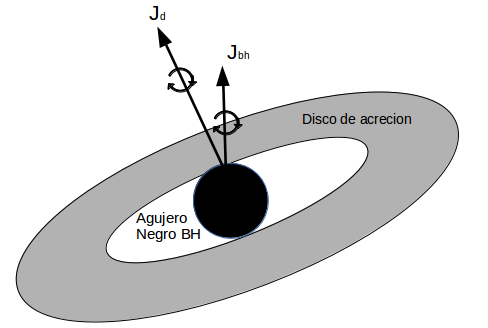
\includegraphics[scale=.35]{./figures/4_Modelo_Spin/Modelo_disco_bh.png}
\figcaption{\emph{Estructura del sistema BH y disco de acreción ambos rotantes y desalineados.}}\label{fig: desaliniamineto_bh_disco}
\end{center}

%------------------------------------------------
    \subsubsection{Acreción de gas en discos desalineados}
    \label{subsubsec: Acrecion gas desaliniado}
%------------------------------------------------
Siguiendo lo anteriormente expuesto, se tiene un disco de acreción que orbita alrededor de un BH. Los dos sistemas al estar rotando presentan un momemtum angular ${\bf{J}}_{bh}$ y ${\bf{J}}_{d}$. Gracias al análisis y resultados en \ref{subsec: Acrecion_gas} es posible asumir que la evolución del espín del BH, depende de la masa acretada por el mismo, ecuación (\ref{eq: espin_final a^f}). El proceso de acreción y cantidad de masa acumulada trasciende el análisis que se pretende realizar, sin embargo es posible tener un estimativo de estos procesos a partir de lo siguiente: Considerar el caso más general, donde se tiene que el disco de acreción rota en un plano diferente al plano ecuatorial del BH (los espines están desalineados), (ver figura \ref{fig: desaliniamineto_bh_disco}). Al considerar este sistema se tiene entonces, que el disco de acreción genera un torque debido al efecto Lense-Thirring (LT) producto de la rotación del BH. El efecto LT puede ser puede ser escrito de la forma:
%
\begin{align}
    \frac{\partial {\bf{L}}}{\partial t}={\bf{\Omega}}_{p}\times{\bf{L}}\,,
    \label{eq: lense-Thirring}
\end{align}
%
donde ${\bf{L}}$ es el momentum angular por unidad de área del disco y ${\bf{\Omega}}_{p}$ es rata de precesión, definida de la forma:
%
\begin{align}
    {\bf{\Omega}}_{p}=\frac{2G}{c^{2}}\frac{{\bf{J}}_{bh}}{R^{3}}\,,
\end{align}
%
donde $R$ es la distancia al BH \cite{pringle1992}. La viscosidad del disco determina altamente la evolución de los espines, entre más grande sea la viscosidad del disco, menor su tiempo de alineación, pero si es lo suficientemente alta, las partículas del interior generan otro disco deformado (warp) (ver figura \ref{fig: sistema con zona warp}), que se alinea con el espín del BH. Por tanto, se hace necesario introducir las escalas de tiempo que brindan información de la dinámica del sistema con alta viscosidad: Se introduce el tiempo de escala de acreción $t_{acc}\equiv R^{2}/\nu_{1}(R)$, indicando el tiempo que demora el gas del disco en caer al BH de manera paralela; el tiempo de escala warp $t_{warp}\equiv R^{2}/\nu_{2}(R)$, que equivale al tiempo de propagación de la deformación en dirección normal.  
%
\begin{center}
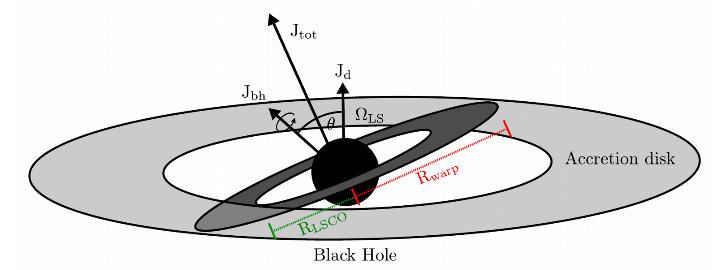
\includegraphics[scale=.4]{./figures/4_Modelo_Spin/Sistema_con_region_warp.png}
\figcaption{\emph{Esquema del sistema donde se ha dado una región warp. Se observan los diferentes espines de cada objeto, el radio warp, radio de la LSO. \cite{Bustamante2018b}}}\label{fig: sistema con zona warp}
\end{center}
%
Sin embargo, el plano ecuatorial del disco warp\footnote{disco interno que es deformado por los torque de marea producto de la alta viscosidad en el disco de acreción.} no mantiene la misma dirección, este precesa al rededor del plano ecuatorial de BH. El tiempo de precesión esta definido como:
%
\begin{align}
    t_{prec}= \frac{2\pi}{{\bf{\Omega}}_p(R)}\,.
\end{align}

Las escalas de tiempo permiten indicarnos si el torque producto del efecto LT, puede alinear los espines. La condición necesaria para el alineamiento es $t_{prec}\lesssim t_{warp}$ \cite{natarajan1999}. A partir de estas, es posible obtener el tamaño del disco deformado $R_{warp}$, en términos del radio de Schwarzschild $R_{Schw}$, el cual se puede escribir de la forma \cite{volonteri2007}:
%
\begin{align}
    \frac{R_{warp}}{R_{Schw}}=3.6\times 10^{3}a^{5/8}\left(\frac{M_{bh}}{10^{8}M_{\odot}} \right)^{1/8}f^{-1/4}\left(\frac{\nu_{2}}{\nu_{1}} \right)^{-5/8}\alpha^{-1/2}\,,
\end{align}
%
donde $f\equiv L/L_{Edd}$ es el radio de Eddington, $L_{Edd}=4\pi GM_{bh}c/\kappa$ es  la luminosidad de Eddington, con $\kappa\sim 0.3 [cm^{2}g^{-1}]$ siendo el scatering por opacidad de los electrones, y $L=\epsilon_{r}\dot{M}c^{2}$ es la luminosidad, con $\dot{M}$ la rata de acreción total y $\alpha$ es parámetro de viscosidad Shakura–Sunyaev.

La región warp\footnote{región deformada ubicada dentro del disco warp} proporciona bastante información sobre la evolución del BH. De esta región se puede inferir la cantidad de materia acretada por el BH $\dot{M_{bh}}$, la materia acretada lleva consigo momentum angular el cual también es consumido por el BH
%el cual sera transferido de manera directa como momentum angular
\cite{volonteri2007}. La masa warp se calcula a partir de $M_{warp}=\dot{M}t_{acc}(R_{warp})$, donde el tiempo de acreción en la región warp se calcula de la forma:
%
\begin{align}
 t_{acc}=\frac{R^{2}_{warp}}{\nu_{1}} = 3 \times10^{6}a^{7/8} \left(\frac{M_{bh}}{10^{8}M_{\odot}} \right)^{11/8}\times f^{-3/4}\left( \frac{\nu_{2}}{\nu_{1}}\right)^{-7/8}\alpha^{-3/2}\,\, \textit{yr}.
\end{align}
%
La relación entre las viscosidades $\nu_1$ y $\nu_2$ determina el tipo de proceso, acreción ó alineación del warp. Para un disco delgado se debe cumplir que $H/\alpha < a \ll 1$. En este trabajo se considera la relación $\nu_{2}/\nu_{1}=2(1+7\alpha)/(\alpha^{2}(4+a^{2}))$ \cite{ogilvie1999} , la cual cumple la condición $\nu_{2}/\nu_{1}\approx 1/\alpha^{2}$ \cite{papaloizou1983}. Bajo la relación asumida se obtiene que $t_{warp}< t_{acc}$, lo cual implica que el disco de la región warp se alinea con el plano ecuatorial del BH en una escala de tiempo menor que la escala de tiempo de acreción de masa. Anteriormente se había dicho que calcular la masa acretada por el BH no era trivial, sin embargo es posible suponer de muy buena manera que la masa warp equivale a la masa acretada en un único episodio $M_{d}$, al usar la ecuación (\ref{eq: Masa_acretada}) \cite{Bustamante2018b} se puede determinar la masa final del BH, necesaria para calcular la evolución del espín del BH (\ref{eq: espin_final a^f})
%
\begin{align}
 M_{d}= \frac{M_{bh}^{f}-M_{bh}}{1-\epsilon_{r}}\,.
 \label{eq: Masa_acretada}
\end{align}
%
%------------------------------------------------
    \subsubsection{Alineamiento o anti-alineamiento del espín}
    \label{subsubsec: Aling_Spin}
%------------------------------------------------

Los procesos que ocurren con respecto a la acreción de gas (sec \ref{subsec: Acrecion_gas}) determinan de una manera considerable la evolución del espín del sistema en general ${\bf{J}}_{tot}$. Recordando lo mencionado en la parte inicial de esta sección, se pude decir que el parámetro de espín $a$ también juega un papel importante en el proceso de alineamiento, proporcionando la dirección de rotación del sistema disco-BH. \cite{king2005} indica que para máxima contra-rotación\footnote{El BH rota en dirección contraria al disco} $a=-1$, con radio de orbita estable $r_{lso}=9$, y para máxima co-rotación\footnote{El BH rota en la misma dirección del disco} $a=1$ con $r_{lso}=1$ (ver figura \ref{fig: contra-rotacion y co-rotacion}). %se tiene entonces que a medida que aumenta $a$ disminuye $r_{lso}$ (ver figura \ref{fig: contra-rotacion y co-rotacion}). 
Al usar la ecuación (\ref{eq: eficiencia radiativa}) se obtiene que la eficiencia radiativa $\epsilon_{r}$ depende inversamente de $r_{lso}$ (ver figura \ref{fig: eficiencia_radiativa }), entonces si $r_{lso}$ crece, la eficiencia $\epsilon_{r}$ disminuye. Como ya se había expuesto, $\epsilon_{r}$ indica cuanta materia es expulsada en forma de energía, entonces conforme $\epsilon_{r}$ crece, menos aporta al momentum angular y al proceso de acreción del sistema. Por lo tanto al ser el sistema contra-rotante el que experimenta una eficiencia radiativa menor, producto del  gran tamaño de la orbita $r_{lso}$ (ver figura \ref{fig: eficiencia_radiativa }) 
%producto del signo de $a$
, es el proceso que más aporta al momentum angular y por ende a la evolución del espín. 

\begin{center}
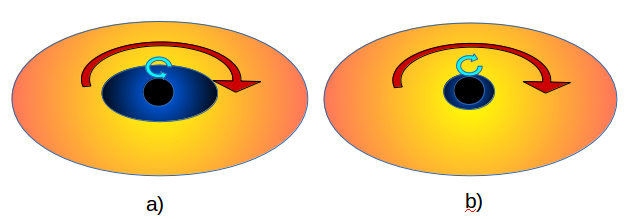
\includegraphics[scale=.35]{./figures/4_Modelo_Spin/Co-rotacion_contra-rotacion.png}
\figcaption{\emph{Comparación entre un sistema que co-rotante (b) y contra-rotante (a). Se observa que cuando es contra-rotante ($a\to -1$)} el radio $r_{lso}\to 9$, y de forma contraria si es co-rotante ($a\to 1$) el radio $r_{lso}\to 1$.}\label{fig: contra-rotacion y co-rotacion}
\end{center}
\begin{center}
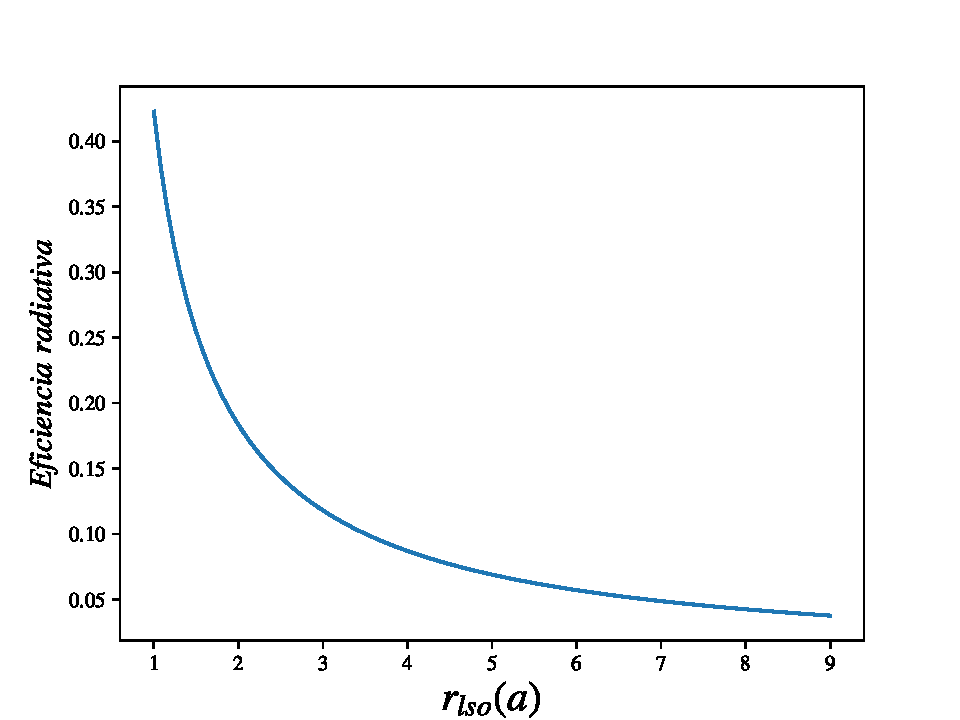
\includegraphics[scale=.5]{./figures/4_Modelo_Spin/eficiencia_radiativa.pdf}
\figcaption{\emph{Dependencia entre el radio de ultima orbita estable $r_{r}$ con la eficiencia radiativa $\epsilon_{lso}$, se observa que cuando $r_{lso}$ es mínimo la eficiencia es máxima, que corresponde a la máxima co-rotación $a=1$, indicando que gran parte del material se pierde y no contribuye al espín del sistema. Al observa el otro caso, pasa todo lo contario, siendo el sistema contra-rotante $a=-1$ el que mejor contribuye a la evolución del espín.}}\label{fig: eficiencia_radiativa }
\end{center}
%%************************
%SEria bueno poner las graficas de sebas sobre el la relación entre el tamaño de r, espin a y la eficiencia
%%*************************

Definiendo el espín del sistema de la forma:
\begin{align}
	{\bf{J}}_{tot}= {\bf{J}}_{bh}+{\bf{J}}_{d}
\end{align}
donde ${\bf{J}}_{d}$ es el momentum angular o espín del la región warp, se define el ángulo de desalineación $\theta$ como el resultado de  ${\bf{J}}_{bh}\cdot{\bf{J}}_{d}$, el cual está acotado ($-1\leq \cos\theta \leq 1$), donde si $\cos \theta \to -1$ indica un anti-alineamiento, y si $\cos \theta \to 1$ indica un alineamiento \cite{king2005}. Al considerar la derivada temporal del producto escalar de  ${\bf{J}}_{bh}$ se obtiene lo siguiente \cite{king2005}:
%
\begin{align}
    \frac{d }{dt}({\bf{J}}_{bh}\cdot {\bf{J}}_{bh})=  \frac{d}{dt}(J_{bh}^{2})= 0 \Rightarrow J_{bh}=cte\,.
\end{align}
%
Esta ecuación indica que ${\bf{J}}_{bh}$ se mueve sobre una esfera. Bajo la suposición anterior es posible concluir que el espín del BH se termina alineando con el espín total. 
%
\begin{align}
    \frac{d}{dt}(\cos\theta_{bh})\geq 0\,,
\end{align}
%
donde $\theta_{bh}$ es el ángulo entre ${\bf{J}}_{bh}$ y ${\bf{J}}_{tot}$, entonces $\theta_{bh}$ debe estar definido entre (0,$\pi/2$) para que se cumpla la condición de la derivada. Esta condición implica que siempre habrá un alineamiento, a medida que $\theta_{bh}$ disminuye en el tiempo, el $\cos\theta_{bh}$ aumenta, hasta llegar a su valor máximo ($\cos( 0)=1$) que indica un alineamiento definitivo.% lo cual implica que a medida que pasa el tiempo la diferencia entre los espines va disminuyendo, hasta llegar a alinearse.

Al saber eventualmente que el momentum angular total y el espín del BH se alinearan, proporciona gran información de la evolución del espín, sin embargo es necesario conocer si el espín del disco se terminara alineando o anti-alineando, para ello, miremos los criterios que dan cabida a ello. Partiendo de la magnitud del momentum angular total
%
\begin{align}
    J^{2}_{tot} = J^{2}_{bh}+J_{d}^{2} -2J_{bh}J_{d}\cos(\pi -\theta)
\end{align}
%
El anti-alineamiento ($\theta\to\pi$) ocurre si y solo si ${\bf{J}}_{bh}^{2}>{\bf{J}}_{tot}^{2}$, que equivale a \cite{king2005}:
%
\begin{align}
    \cos\theta < - \frac{{\bf{J}}_{d}}{2{\bf{J}}_{bh}}\,.   
\end{align}
%
Por lo tanto, gracias a este criterio es posible indicar si el sistema BH-disco está alineado/anti-alineado: si $\theta >\pi/2$ y $2{\bf{J}}_{bh}>{\bf{J}}_{d}$ el BH está anti-alineado, si  $2{\bf{J}}_{bh}<{\bf{J}}_{d}$ hay alineamiento, el cual siempre ocurre cuando el momentum angular del disco sobrepasa al del BH \cite{king2005}.

La magnidtud del momentum angular del disco esta dado por \cite{Bustamante2018b}:
%
\begin{align}
    J_{d}=\int_{warp} \Sigma_{d}\Omega_{k}(R)R^{2}dS \approx M_{d}(GM_{bh}R_{warp})^{1/2}\,,
    \label{eq: magnitid J_disco}
\end{align}
%
donde $\Sigma$ es la densidad superficial del disco, $\Omega_{k}$ es la frecuencia de Kepler y la integral va sobre todo la superficie de la región warp. Se ha asumido que todo el gas que va cayendo al BH esta circulando sobre todo el disco, entonces el momentum angular debería de distribuirse sobre toda la región warp. Este argumento permite encontrar una relación entre el momentum angular del disco y el BH \cite{king2005}.
%
\begin{align}
    \frac{J_{d}}{2J_{bh}}\approx \frac{M_{d}}{aM_{bh}}\left(\frac{R_{warp}}{R_{Schw}} \right)^{1/2}
\end{align}
%
Este criterio permite evaluar cada episodio de acreción, con lo cual se puede conocer si hay alineamiento o anti-alineamiento antes de que se acrete el disco [SEBAS]. 

\begin{center}
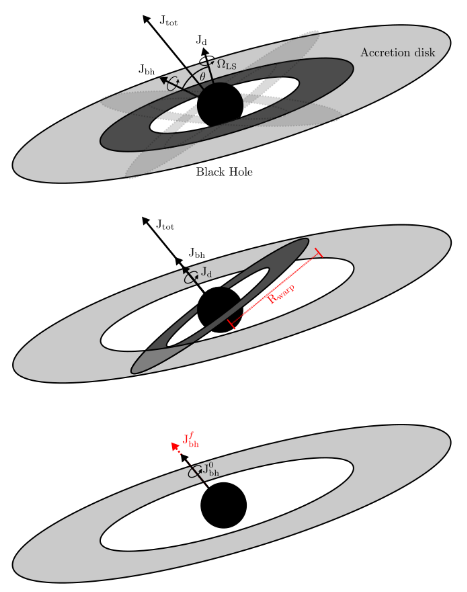
\includegraphics[scale=.5]{./figures/4_Modelo_Spin/evolucion_spin.png}
\figcaption{\emph{ Proceso evolutivo de los espines del sistema. En la figura superior, se tiene el caso inicial donde se formó la región warp, la cual está precesando. La figura del medio presenta el momento en que la región warp se estabiliza, alineando su espín con el espín del BH. La figura inferior muestra el momento final, donde todo los espines se alinean y la masa del disco interno ha sido acretada  \cite{Bustamante2018b}.}}\label{fig: evolucion espin}
\end{center}


%------------------------------------------------
    \subsubsection{Discos auto-gravitantes}
    \label{subsubsec: Disco auto-gravitantes}
%------------------------------------------------
Cuando se llega al caso en el cual la rata de acreción del sistema BH y disco de acreción es muy alta, se genera un disco de acreción aun más grande. En las regiones más externas del disco de acreción se empiezan a formar una zona donde la gravedad  es comparable o mayor al potencial gravitacional generado por el BH, permitiendo el colapso de pequeñas parcelas de gas
%grueso, que al no estar tan cerca al BH, sienten una gravedad propia y empieza a colapsar en pequeñas nubes de gas 
(figura \ref{fig: Sistema auto-gravitante}). Esta región externa comienza a formar estrellas muy masivas que evolucionan rápidamente, que al explotar como súper novas generan vientos  violentos que perturban el sistema, en especial que afectan la dinámica del disco interior de forma caótica. 
%
\begin{center}
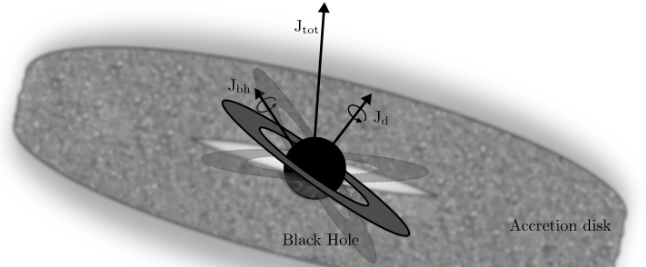
\includegraphics[scale=.3]{./figures/4_Modelo_Spin/Sistema_auto-gravitante.png}
\figcaption{\emph{Modelo del sistema auto-gravitante, en la parte exterior a la región warp se forma una distribución de gas, la cual es gobernada por una dinámica auto-gravitante \cite{Bustamante2018b}.}}\label{fig: Sistema auto-gravitante}
\end{center}
%
Para entender este suceso se hace uso del criterio de estabilidad de Toomre, el cual compara el soporte rotacional del disco contra su propia gravedad \cite{Bustamante2018b}:
%
\begin{align}
    Q\equiv\frac{c_{s}\Omega_{k}}{\pi G\Sigma_{d}}\,,
    \label{eq: estabilidad_Toomre's}
\end{align}
%
%
donde $c_{s}$ es la velocidad del sonido en el gas. En el caso en que $Q\leq 1$ el disco es inestable, esto conduce a la definición un radio de auto-gravedad $R_{sg}$, el cual debe cumplir que $Q(R_{sg})=1$. El radio de auto-gravedad es determinado por \cite{fanidakis2011}:
\begin{align}
    \frac{R_{sg}}{R_{Schw}}=1.5\times 10^{3}\epsilon^{8/27}\left(\frac{M_{bh}}{10^{8}M_{\odot}} \right)^{-26/27}f^{-8/27}\alpha^{14/27}
\end{align}
%
Debido a que $Q$ es un parámetro que decrece monótonamente a medida que crece el radio, la parte exterior al $R_{sg}$, donde no se cumple el criterio de estabilidad de Toomre, esta sujeta a fragmentación, mientras que la parte interior que sí se cumple la condición se genera un disco estable. Solo el material que se encuentra dentro del radio de warp puede transferir momentum angular de forma eficiente, es por eso que solo se incluye los efectos de auto-gravedad si $R_{sa}\leq R_{warp}$. Si se cumple la relación anterior, se debe obtener la relación de la masa que contribuye al momentum angular del sistema, dada por \cite{fanidakis2011}:
%
\begin{align}
    M_{sg} = 2.13\times 10^{5}\epsilon^{-5/27}\left(\frac{M_{bh}}{10^{8}M_{\odot}} \right)^{23/27}f^{5/27}\alpha^{-2/17}M_{\odot}\,.
\end{align}
%
Ahora con los valores de $M_{sg}$ y $R_{sg}$ que al remplazarlos por $M_{d}$ y $R_{warp}$, se puede obtener la evolución del espín del BH en el régimen de auto-gravedad.


%------------------------------------------------
\subsection{Coalesencia de BH's}
\label{subsec:fusion_BHs}
%------------------------------------------------
La otra forma de poder cambiar la dirección y magnitud del espín del BH es a partir de fusiones entre  sistemas binarios de BHs (ver figura \ref{fig: fusion_Bhs}). Este fenómeno es común en procesos de formación jerárquicos, en los cuales dos galaxias colisionan, generando un pozo de potencial donde los dos BHs perteneciente a cada galaxia van a terminar cayendo, y posteriormente fusionándose debido a la fricción dinámica. Entonces al fusionarse los dos BHs, la dirección de cada uno se combina, generando un nuevo espín. Una forma de calcular el espín resultante de la fusión, es usando el ajuste analítico de \cite{rezzolla2008}: 
%
\begin{align}
    a = \frac{1}{(1+q)^{2}}(a_{1}+a_{2}q^{2}+\ell q)\,,
\end{align}
%
donde $a_{1}$ es el parámetro de espín del BH más masivo, $a_{2}$ equivale al parámetro de espín del menos masivo, $q$ es la razón entre las masas $q=M_{2}/M_{1}\leq 1$ y $ {\bf{\ell}} = {\bf{l}}/(M_{1}M_{2})$, donde ${\bf{l}}$ es la diferencia entre el momentum angular orbital ${\bf{L}}$ con el momentum angular de las ondas gravitacionales ${\bf{J}}_{og}$, en un instante antes de la fusión ${\bf{l}}={\bf{J}}-{\bf{J}}_{og}$.

La norma de $\ell$ se obtiene de forma analítica \cite{rezzolla2008}: 
%
\begin{align}
    \ell = \frac{s_{4}}{(1+q^{2})^{2}}(a_{1}^{2}+a_{2}^{2}q^{4}+2{\bf{a_{1}\cdot a_{2}}}q^{2})\\ + \frac{s_{5}\mu + t_{0}+2}{1+q^{2}}(a_{1}\cos\phi_{1}+a_{2}q^{2}\cos\phi_{2})\\ 
    + 2\sqrt{3}+t_{2}\mu+t_{3}\mu^{2}\,,
\end{align}
donde $\phi_{1}(\phi_{2})$ son los ángulos entre $a_{1}(a_{2})$ y $\vec{\ell}$, y $\mu = q/(1+q)^{2}$. Al igual que supone \cite{rezzolla2008}, se considera que la dirección de $\Vec{\ell}$ es paralela con la dirección del momentun angular ${\bf{L=L_{1}+L_{2}}}$ antes de la fusión, el cual es un vector medido en la simulación. Para tener el valor de ${\bf{L}}$ es necesario calcular el centro de masa del sistema binario ${\bf{r}}_{com}$, con esta posición se evalúa el momentum angular de los dos BHs relativo al centro de masa. Se tiene además los valores de los coeficientes: $s_{4}=-0.129$, $s_{5}=-0.384$, $t_{0}=-2.686$, $t_{2}=-3.454$ y $t_{3}=2.353$ \cite{rezzolla2008}.

\begin{center}
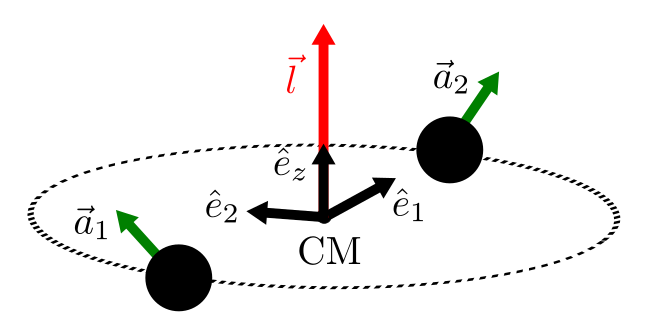
\includegraphics[scale=.3]{./figures/4_Modelo_Spin/fusion_BHs.png}
\figcaption{\emph{Sistema binario de BHs, donde cada uno tiene un espín característico y la contribución de cada uno conlleva a un momentum angular del sistema $\vec{\ell}$ \cite{Bustamante2018b}}.}\label{fig: fusion_Bhs}
\end{center}















%*************************************************************************

%--------------------- Algoritmo_Modelacion ------------------------
%qqqqqqqqqqqqqqqqqqqqqqqqqqqqqqqqqqqqqqqqqqqqqqqqqqqqqqqqqqqqqqqqqqqqqqqqq
%Quote
\begin{savequote}[50mm]
%‘‘El cosmos es todo lo que es, todo lo que fue y todo lo que será. Nuestras 
%más ligeras contemplaciones del cosmos nos hacen estremecer: Sentimos como 
%un cosquilleo nos llena los nervios, una voz muda, una ligera sensación como
%de un recuerdo lejano o como si cayéramos desde gran altura. Sabemos que nos
%aproximamos al más grande de los misterios.’’
%\qauthor{Carl Sagan}
\end{savequote}
%qqqqqqqqqqqqqqqqqqqqqqqqqqqqqqqqqqqqqqqqqqqqqqqqqqqqqqqqqqqqqqqqqqqqqqqqq




%#########################################################################
\chapter{Algoritmo y Modelación.}
\label{cha:Algoritmo y Modelación}














%***********************************************************************
			
%----------- Clasificación entorno cosmológico--------------
%qqqqqqqqqqqqqqqqqqqqqqqqqqqqqqqqqqqqqqqqqqqqqqqqqqqqqqqqqqqqqqqqqqqqqqqqq
%Quote
\begin{savequote}[60mm]
"No me parece que este universo fantásticamente maravilloso, pueda simplemente ser un escenario para que Dios vea a los seres humanos luchar por el bien y el mal."
\qauthor{Richard Feynman}
\end{savequote}
%qqqqqqqqqqqqqqqqqqqqqqqqqqqqqqqqqqqqqqqqqqqqqqqqqqqqqqqqqqqqqqqqqqqqqqqqq




%#########################################################################
\chapter{Alineamiento de AGNs con su entorno a gran escala}
\label{cha:cosmic_web}

En esta sección se presentan los resultados obtenidos en la búsqueda de posible alineamiento del espín de los AGNs con el entorno cosmológico al cual pertenecen. Con el fin de poder llevar a cabo este propósito, se hace uso de dos simulaciones cosmológicas ({\it{cosmo01}} y {\it{cosmo02}}) y el método T-Web, donde se usan los autovalores y autovectores. A continuación se presentan las características de las simulaciones y  los resultados obtenidos.

%------------------------------------------------
\section{Características de las simulaciones}
\label{sec: propiedades en las simulaciones}
%------------------------------------------------

En las simulaciones hay parámetros o valores que dan información de la dinámica del sistema, que arrojan criterios suficientes para decidir si lo obtenido está en concordancia con los modelos físicos propuestos. 
Conforme a esto, se pretende realizar un análisis a la distribución de masa (función de masa) de los halos, BHs y de masa estelar del halo. 

Debido a que no todos los halos hospedan un BH en su interior, fue necesario descartar los halos que no cumplen con esta condición. Esto reduce en gran manera la cantidad de galaxias a estudiar, sin embargo es suficiente para realizar un análisis adecuado.

%------------------------------------------------
    \subsection{ Función de distribución de masa}
    \label{subsec: funcion de masa}
%------------------------------------------------
La función de masa es uno de los parámetros de control más contundentes en el análisis de los modelos y simulaciones. Bajo la teoría de formación y evolución de galaxias se tiene que los objetos con baja masa son más abundantes, debido que en los procesos evolutivos en las galaxias presentan interacción jerárquica, las galaxias más masivas tiene una mayor probabilidad en fusionarse con otras debido a su gran potencial gravitacional, esto hace que las galaxias más densas se terminen fusionando y así se disminuya su población. Con base a esto la función de masa de las galaxias (halos, BHs y masa estelar) debe decrecer a medida que se aumentan las masas, i.e., La cantidad de objetos disminuye a medida que aumenta la masa, es menos probable encontrar BHs muy masivos.
%
\begin{figure}
\centering
\subfloat{
%\label{fig: función de masa BHs}
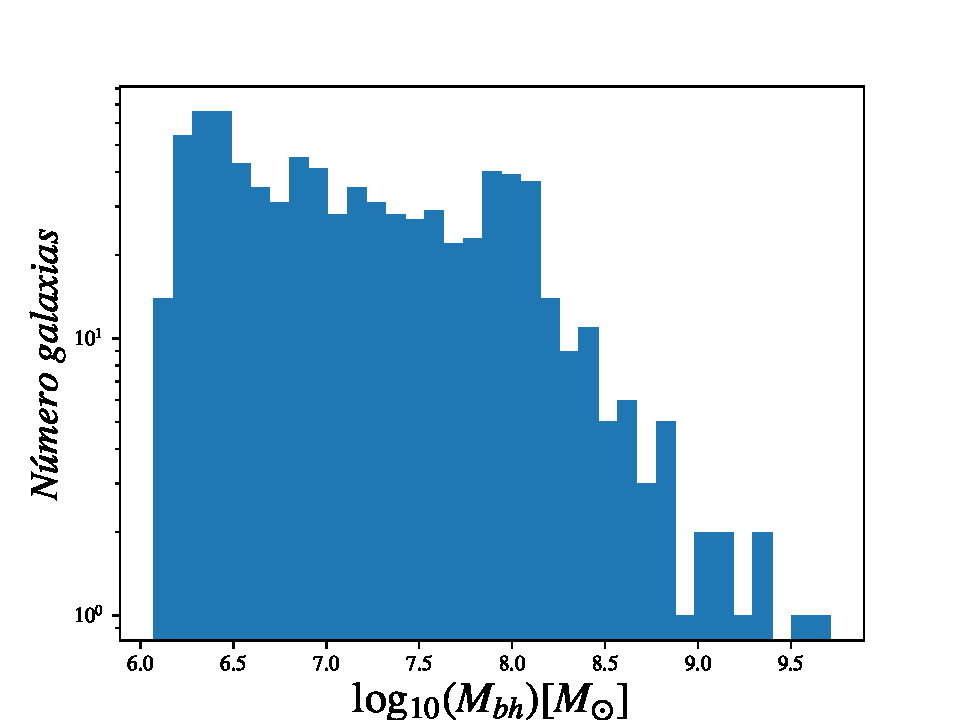
\includegraphics[width=0.6\textwidth]{./figures/6_Resultados/cosmo01/histo_Mass_bh.pdf}}
\subfloat{
%\label{fig: función de masa halos}
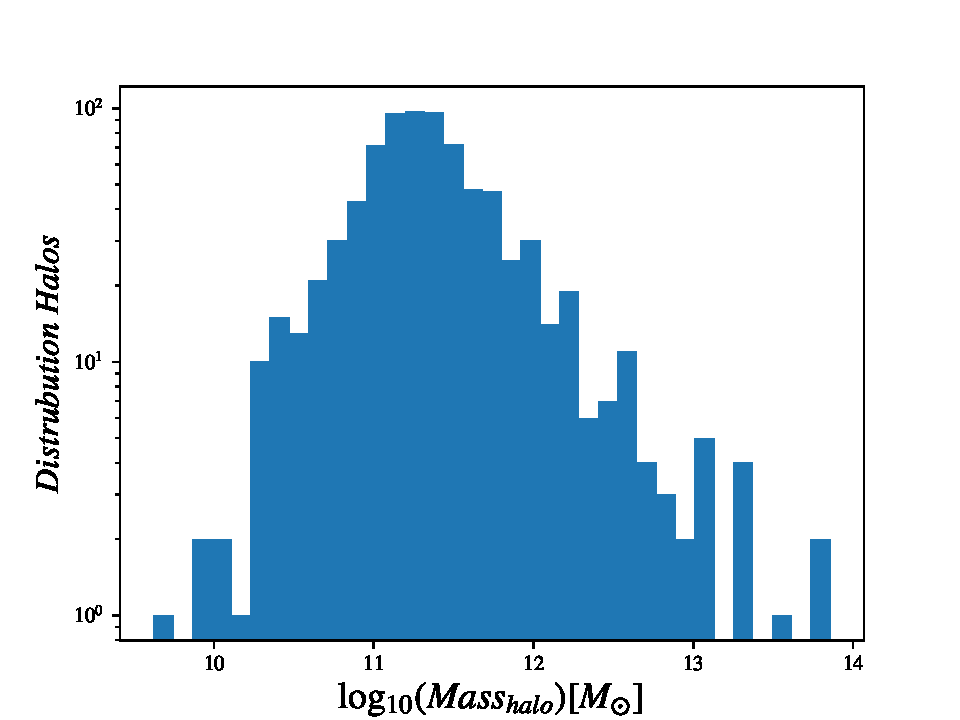
\includegraphics[width=0.6\textwidth]{./figures/6_Resultados/cosmo01/histo_Mass_halos.pdf}}
\subfloat{
%\label{fig: función de masa estelar}
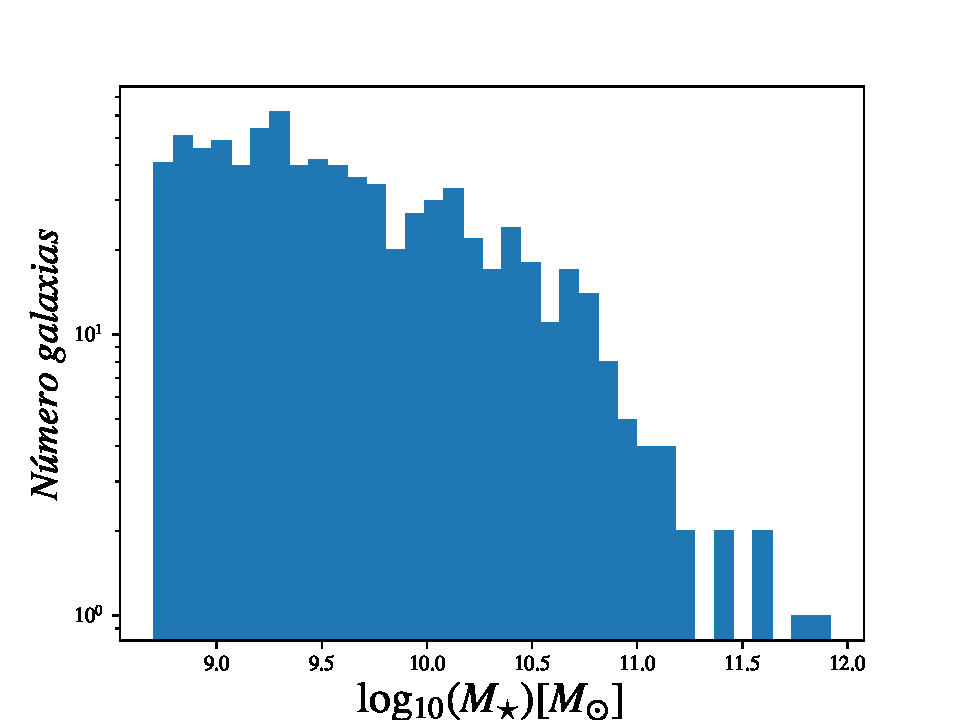
\includegraphics[width=0.6\textwidth]{./figures/6_Resultados/cosmo01/histo_Mass_stelar.pdf}}
\caption{\emph{Funciones de distribución de masa para agujeros negros, halos y masa estelar, estas información da cuenta del número de objetos con una masa determinada, esto se realizo para {\it{cosmo01}}. }}
 \label{fig: Funciones de masa cosmo01}
\end{figure}
 %%%%%%%%%%%%%%%%%%%%%%%%%%%%%%%%%%%%%%%%%%%
\begin{figure}
\centering
\subfloat{
%\label{fig: función de masa BHs}
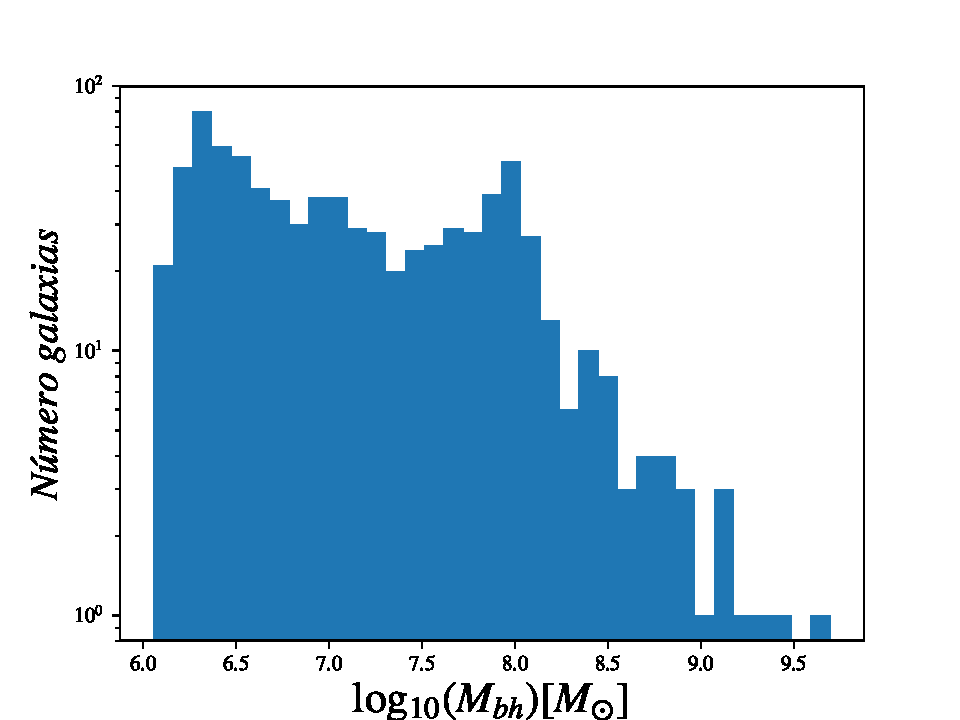
\includegraphics[width=0.6\textwidth]{./figures/6_Resultados/cosmo02/histo_Mass_bh.pdf}}
\subfloat{
%\label{fig: función de masa halos}
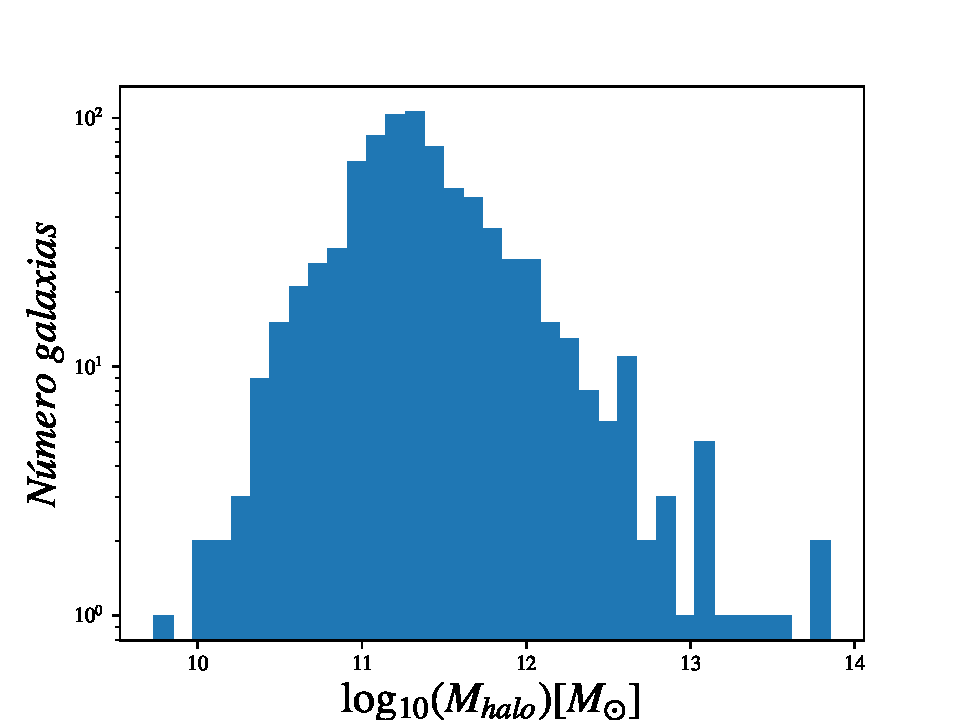
\includegraphics[width=0.6\textwidth]{./figures/6_Resultados/cosmo02/histo_Mass_halos.pdf}}
\subfloat{
%\label{fig: función de masa estelar}
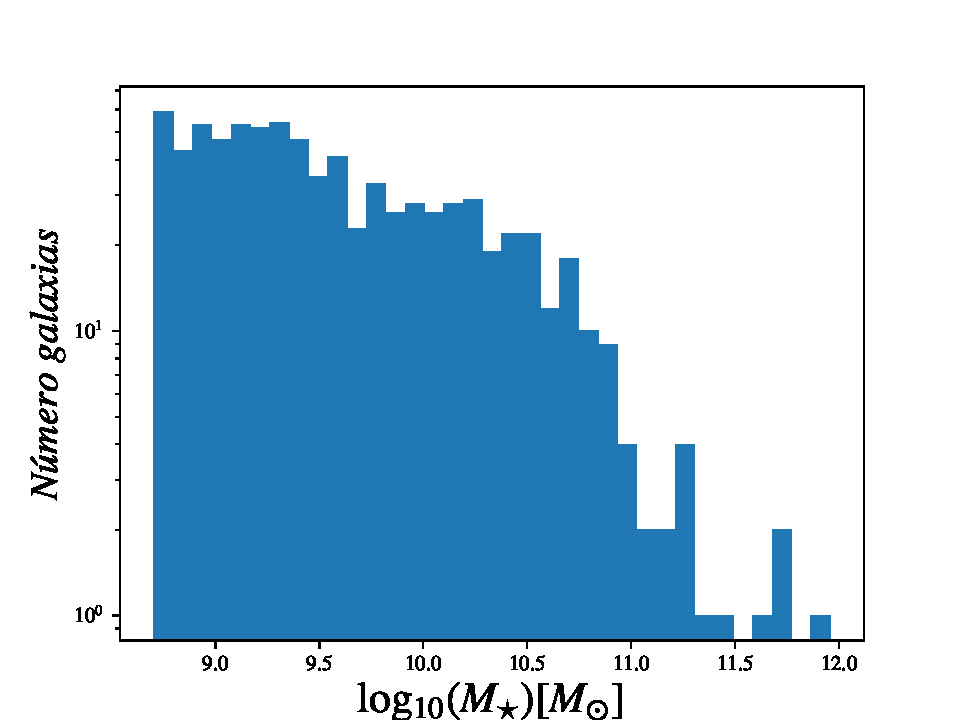
\includegraphics[width=0.6\textwidth]{./figures/6_Resultados/cosmo02/histo_Mass_stelar.pdf}}
\caption{\emph{Funciones de distribución de masa para agujeros negros, halos y masa estelar, estas información da cuenta del número de objetos con una masa determinada, esto se realizo para {\it{cosmo02}}.}}
 \label{fig: Funciones de masa cosmo02}
\end{figure}
%

Al observar las figuras (\ref{fig: Funciones de masa cosmo01} y \ref{fig: Funciones de masa cosmo02}), es posible concluir que los resultados de la simulación son congruentes con la teoría y con las observaciones. Para despreciar los posibles errores producto de la baja resolución en galaxias de baja masa, solo se consideraran sistemas en los cuales las masa estelar sea mayor a $5\times 10^{8}M_{\odot}$. Este criterio hace que la distribución de masa para los halos presente una extraña forma, en esta gráfica se nota la relación existente entre la masa del halo y la masa estelar. A medida que aumenta la masa del halo aumenta la masa estelar del halo. 
%que los halos de baja masa presentan una gran número de halos con masa estelar menor a $5\times 10^{8}M_{\odot}$, pero a medida que aumenta la masa del halo el número de halos con masa estelar del halo es menor al criterio disminuye. 
%se puede observar una relación entre la masa del halo y la masa estelar. A medida que aumenta la masa del halo aumenta la masa del halo. 

A parte de la función de distribución de masa, es posible usar otros criterios que dan información de la simulación y de su veracidad. 

La teoría sobre la formación de galaxias indica la existencia de una relación lineal entre la masa estelar de una galaxia y la masa del BH huésped, i.e., las galaxias que poseen una masa estelar considerable poseen un BH con una masa considerable también. Por tanto las simulaciones debe reproducir este resultado teórico y observacional. Al observa las figuras (\ref{fig: Mass_bhVsMass_stelar}), es posible observar que las simulaciones bajo este criterio, también reproducen lo esperado. 
%
 \begin{figure}
 \centering
  \subfloat{
   %\label{fig: mass_bhVsmass_stelar}
    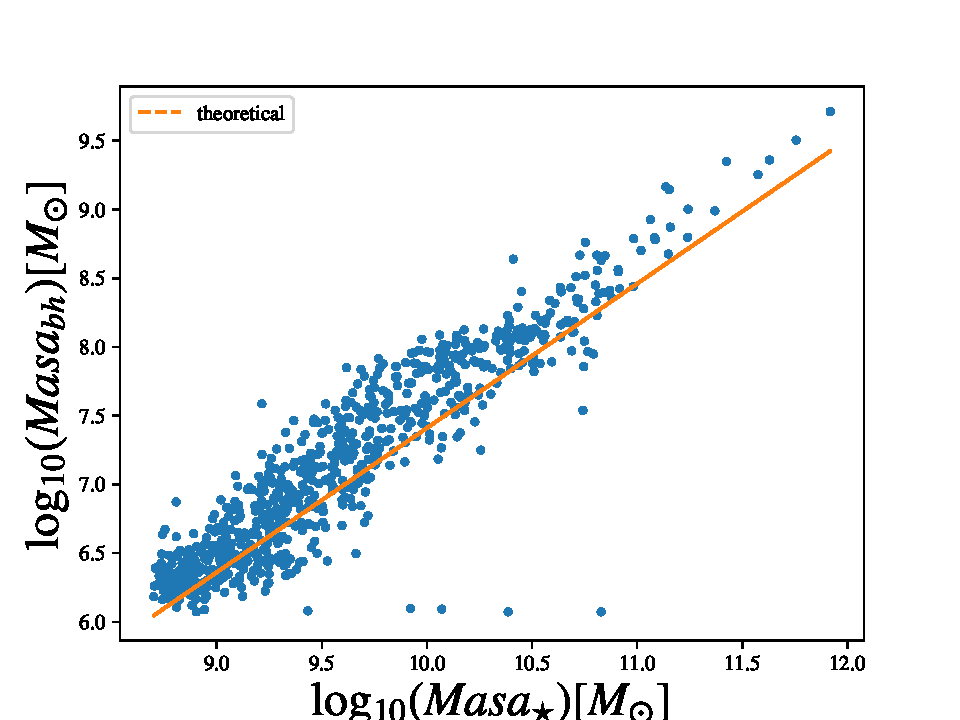
\includegraphics[width=0.49\textwidth]{./figures/6_Resultados/cosmo01/Mass_bhVsMass_stelar_halo.pdf}}
  \subfloat{
   %\label{fig: función de masa halos}
    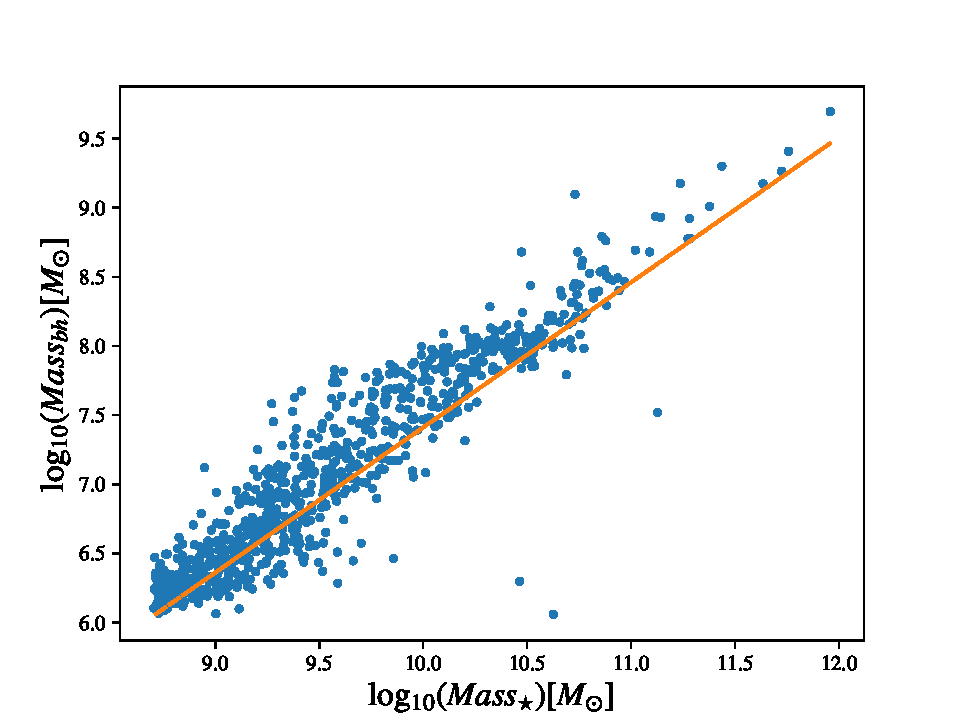
\includegraphics[width=0.49\textwidth]{./figures/6_Resultados/cosmo02/Mass_bhVsMass_stelar_halo.pdf}}
 \caption{\emph{Relación Masa BH y Masa estelar, según los resultados observacionales hay una dependencia lineal entre la masa del BH y la masa estelar para cada galaxia. La imágen de la derecha pertenece a {\it{cosmo01}} y el de la izquierda a {\it{cosmo02}}. La linea naranjada es la teórica \cite{McConnell2013}, con la cual se puede asegurar que la simulación es consistente con lo observacional.}}
 \label{fig: Mass_bhVsMass_stelar}
\end{figure}
%
%------------------------------------------------
    \subsection{ Distribución de galaxias en el entorno cosmológico}
    \label{subsec: Distribucion de galaxias}
%------------------------------------------------

La distribución de las galaxias en el entorno cosmológico son determinantes en el resultado final de este trabajo. Es necesario entonces poder concluir que los resultados obtenidos por las simulaciones reproduzcan las observaciones. Haciendo uso de método de T-Web, se extraen los autovalores $\lambda_{i}$, los autovectores $\vec{e}_{i}$ y la sobre densidad $\delta$. 

Como se explico en la sección (\ref{subsec: Metodo_T-web}),  los autovalores son los responsables de clasificar los entornos y con ello el entorno al cual pertenecen las galaxias. Es necesario contrastar que la distribución de galaxias debe ser equivalente al mapa de sobre densidades. 

%(ANALISIS Y GRAFICA DEL LA DENSIDAD CON )

Al observar las distribución de BHs en el espacio, se observa que gran parte de los BHs se ubica en los cluster o filamentos. Este resultado puede ser contrastado con el valores de los autovalores $\lambda_{i}$, ver figura (\ref{fig: Histograma Autovalores}). También se puede concluir lo siguiente:  $\lambda_{1}\geq 0$,  $\lambda_{2}\geq 0$ y $\lambda_{3}$ esta acotado entre $-10 \leq \lambda_{3}\leq 10$, mayormente con valores positivos, reproduciendo estructuras con características de filamentos o clusters. 
%
\begin{center}
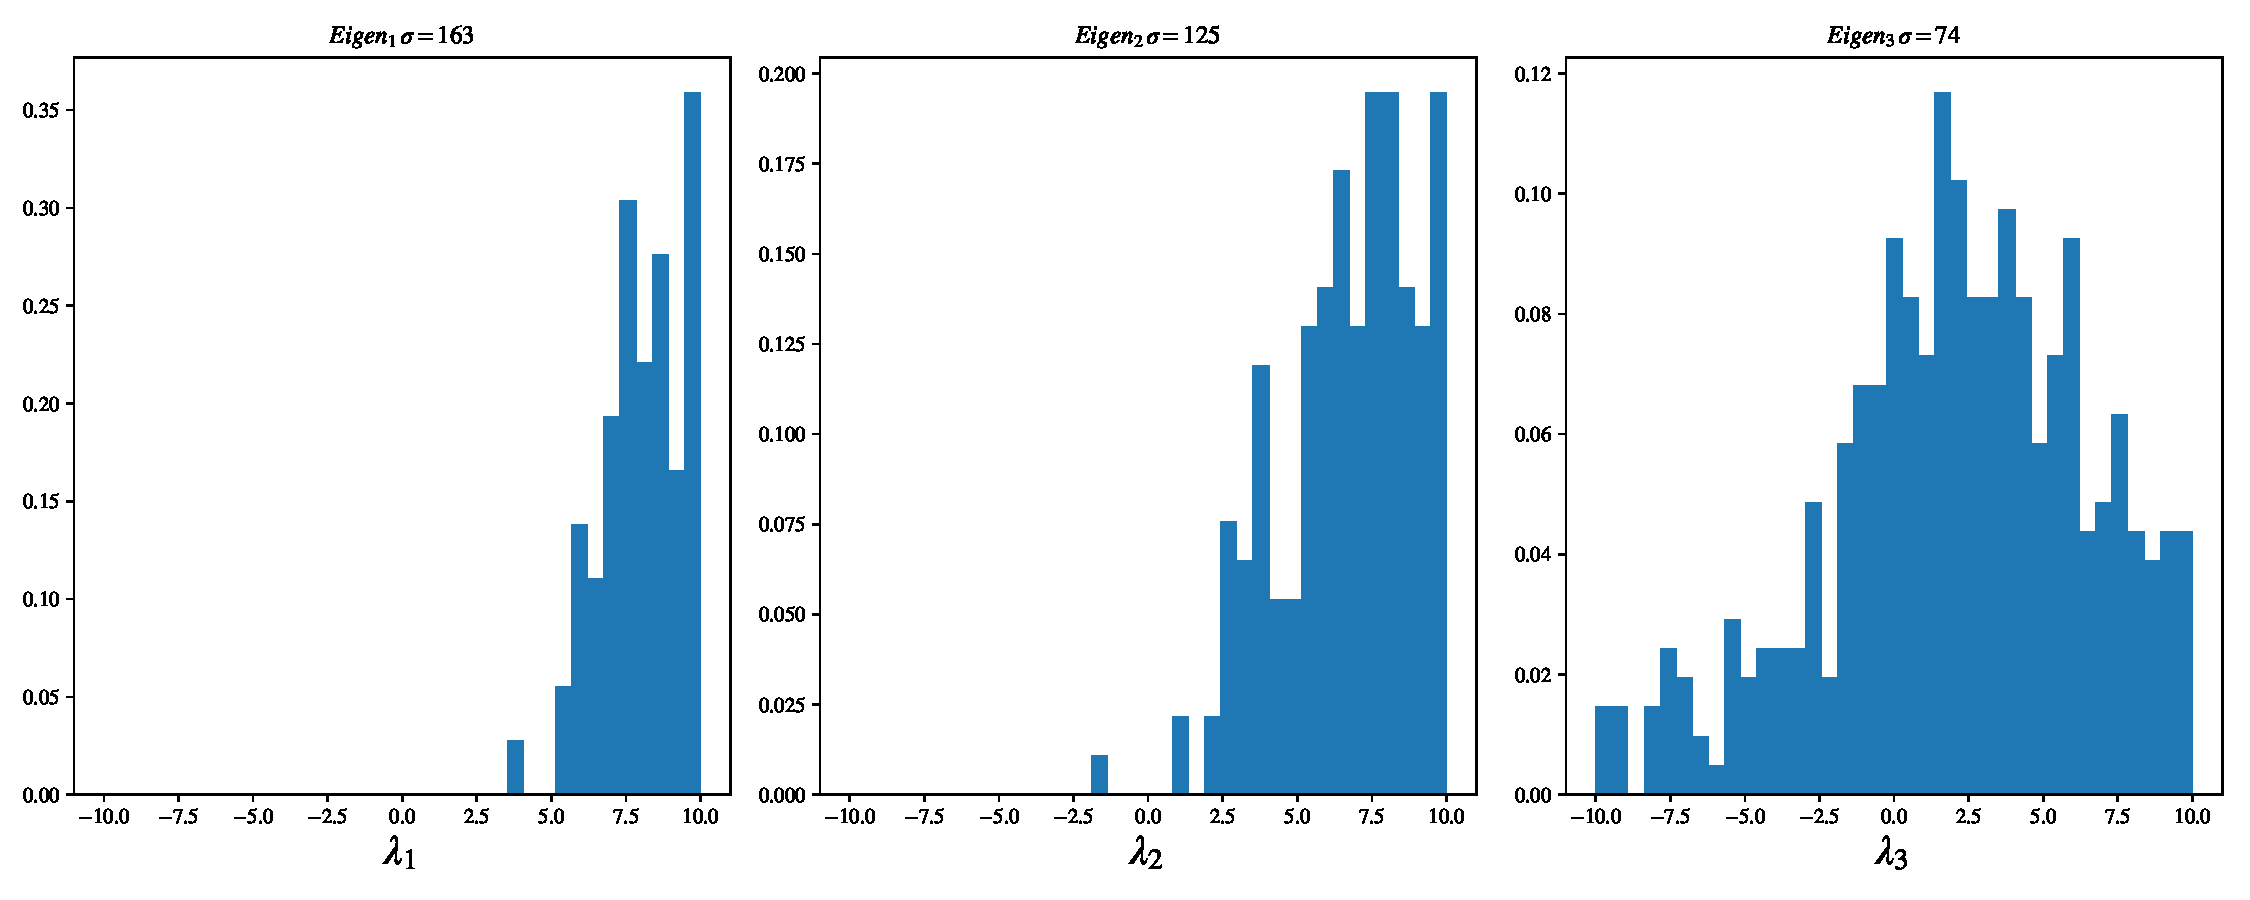
\includegraphics[scale=.38]{./figures/6_Resultados/cosmo01/histograma_autovalores2.pdf}
\figcaption{\emph{Histograma de los autovalores $\lambda_{i}$, que proporcionan información acerca de la clasificación y dinámica de la simulación a gran escala. Estos autovalores son obtenidos del método de  T-Web, calculando la diagonal de la matriz Hessiana.}}
\label{fig: Histograma Autovalores}
\end{center}
%




%------------------------------------------------
\section{ Alineamiento}
\label{sec: Alineamiento}
%------------------------------------------------

En esta sección se presentan los resultados que darán pie a argumentar si existe alguna relación entre la orientación del espín del BH y el entorno. Se mostraran los resultados logrados con varios sistemas (momentum angular de BHs, discos de acreción, halos y entorno), encaminados a comparar los resultados y poder dar respuesta a la pregunta planteada en este proyecto. 

Recordando la estructuración de las galaxias, para la cual se afirma que todas galaxias cuentan con un halo, que en su interior presenta un BH, cuando este está "activo" se denomina AGN. Se consideran tres parámetros fundamentales para cada galaxia: para los halos se estudiará la masa estelar contenida en el halo, posición y momentum angular; para los AGN se estudiará el SMBH y el disco de acreción, del SMBH se extrae la masa, espín y posición; del disco de acreción el momentum angular. Estos parámetros fueron calculados usando la teoría de evolución de espín (ver capitulo \ref{cha:Modelo de Spin}) y usando el código {\it{Arepo}} (ver sección \ref{sec: codigo arepo} ) que reproduce la evolución y formación de galaxias. 

Para estudiar la alineación se utiliza como parámetro el $\cos (\theta)$, el cual está acotado entre -1 y 1 (ver sección \ref{subsubsec: Aling_Spin}). Partiendo de esto se argumenta que hay alineamiento sii  $\cos (\theta) \to 1$, anti-alineamiento si $\cos (\theta)\to -1$, ortogonalidad si $\cos (\theta)\to 0$ y si $\cos (\theta)\to \pm 0.5 $ no es posible concluir algo. Con base en esto se procede a calcular la relación entre los momentum angulares de cada sistema, a continuación se nombrar los ángulos con los cuales se busca encontrar alguna relación:

$\theta$ : ángulo entre el espín del BH ${\bf{J_{bh}}}$ y el autovector tres $\vec{\bf{e}}_{3}$.

$\alpha$ : ángulo entre el espín del BH ${\bf{J_{bh}}}$  y el disco de acreción ${\bf{J_{d}}}$ .

$\beta$ :  ángulo entre el espín del BH ${\bf{J_{bh}}}$ y el halos ${\bf{J_{halo}}}$\\

Una vez definidos los ángulos, procedamos a presentar una serie de resultados que contrastados con la teoría aportaran a la solución de la respuesta central del texto. Como primera parte, identifiquemos cómo se comportan las alineaciones en la simulación, para esto se determinará la distribución de ángulos de alineamientos. 

%(HABLAR QUE DE AHORA EN ADELANTE SOLO SE VA HA CONSIDERAR COSMO01)
Valiéndonos de los resultados logrados con las simulaciones y de la teoría de evolución de espín, consideramos que la simulación que da cuenta de los sucesos de una forma más general físicamente es la simulación con acreción caótica. Por lo tanto a partir de acá los resultados reportados serán meramente resultados de obtenidos con {\it{cosmo01}}. 

%%%%*****************************************%%%%%%%%%%%%%%%


%%%%%%%%%%%%%%%%%%%%%%%%%%%%%%%%%%%%%%%%%%%%%%%%%%%%%

Una vez visto estas relaciones, procedamos a estudiar como se comporta $\theta$. La relaciones que se obtengan de $\theta$ son de gran importancia, ya que está es la responsable de indicar si hay o no alineamiento con el entorno. Por tanto observemos que ocurre con la distribución de $\cos \theta$ para diferentes autovalores $\lambda_{i}$.
%
\begin{center}
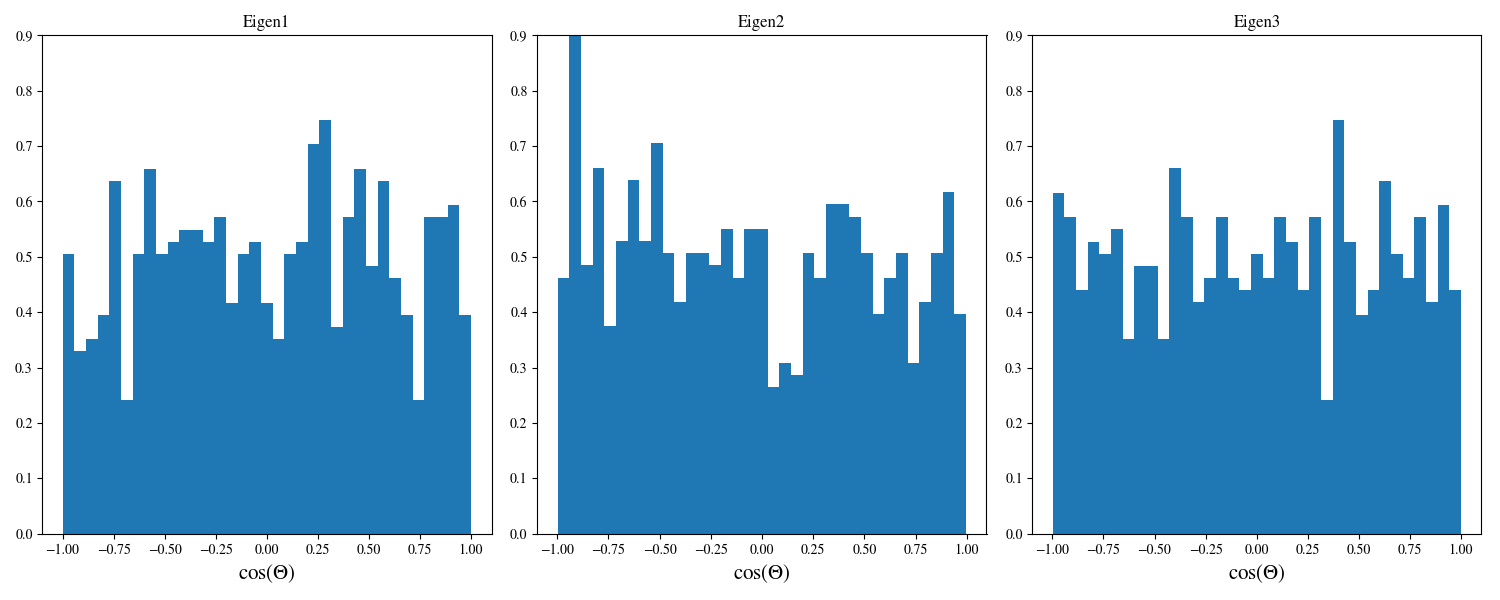
\includegraphics[scale=.35]{./figures/6_Resultados/cosmo01/histograma_cos_theta.png}
\figcaption{\emph{Distribución de $\cos \theta$ para cada BH en la simulación de cosmo01. Se observa una gran aleatoriedad debida que no se cuenta con un gran número de datos y porque se está considerando BHs alineados y no alineados.}}\label{fig: histograma costeta}
\end{center}
%
Al observar la figura (\ref{fig: histograma costeta}) se evidencia una gran aleatoriedad en la distribución de $\cos\theta$, la razón de ellos es que la distribución considera tanto BHs alineados como no alineados. Además se evidencia que para los tres autovalores ocurre lo mismo, una gran aleatoriedad. Para deshacernos de este problema se hace necesario estudiar el comportamiento de los BHs en regiones especificas de la simulación, donde se tenga alguna idea de un alineamiento.  

Ahora en búsqueda de no estimar objetos no alienados estudiemos entornos particulares, y ver si existe alguna relación entre el parámetro de alineamiento $\cos\theta$ y parámetros relacionados con el entorno, como lo son la masa del BH, la masa estelar del halo, masa del halo y autovectores, en especial $\lambda_{3}$. La teoría de formación de galaxias y estructuras muestra que en regiones de sobre densidad (clusters o filamentos) las galaxias presentan una mayor cantidad de masa  con respecto a las galaxias que se encuentran el regiones de baja densidad, lo cual se puede traducir en una relación directa entre el entorno y la masa de los BHs. Es entonces la masa el criterio usado para encontrar el posible alineamiento. 

La figura (\ref{fig: proyeccion espines}) da cuenta de la discretización que se pretende hacer, para no tener en cuenta los BHs no alineados. Se estiman tres rangos de masas de BH. Al clasificar las galaxias por la masa de su BH, se intenta descartar la contribución de objetos no alineados que puedan producir error o incertidumbre en el resultado final. 

\begin{figure} 
\centering \subfloat{ 
%\label{fig: función de masa BHs}
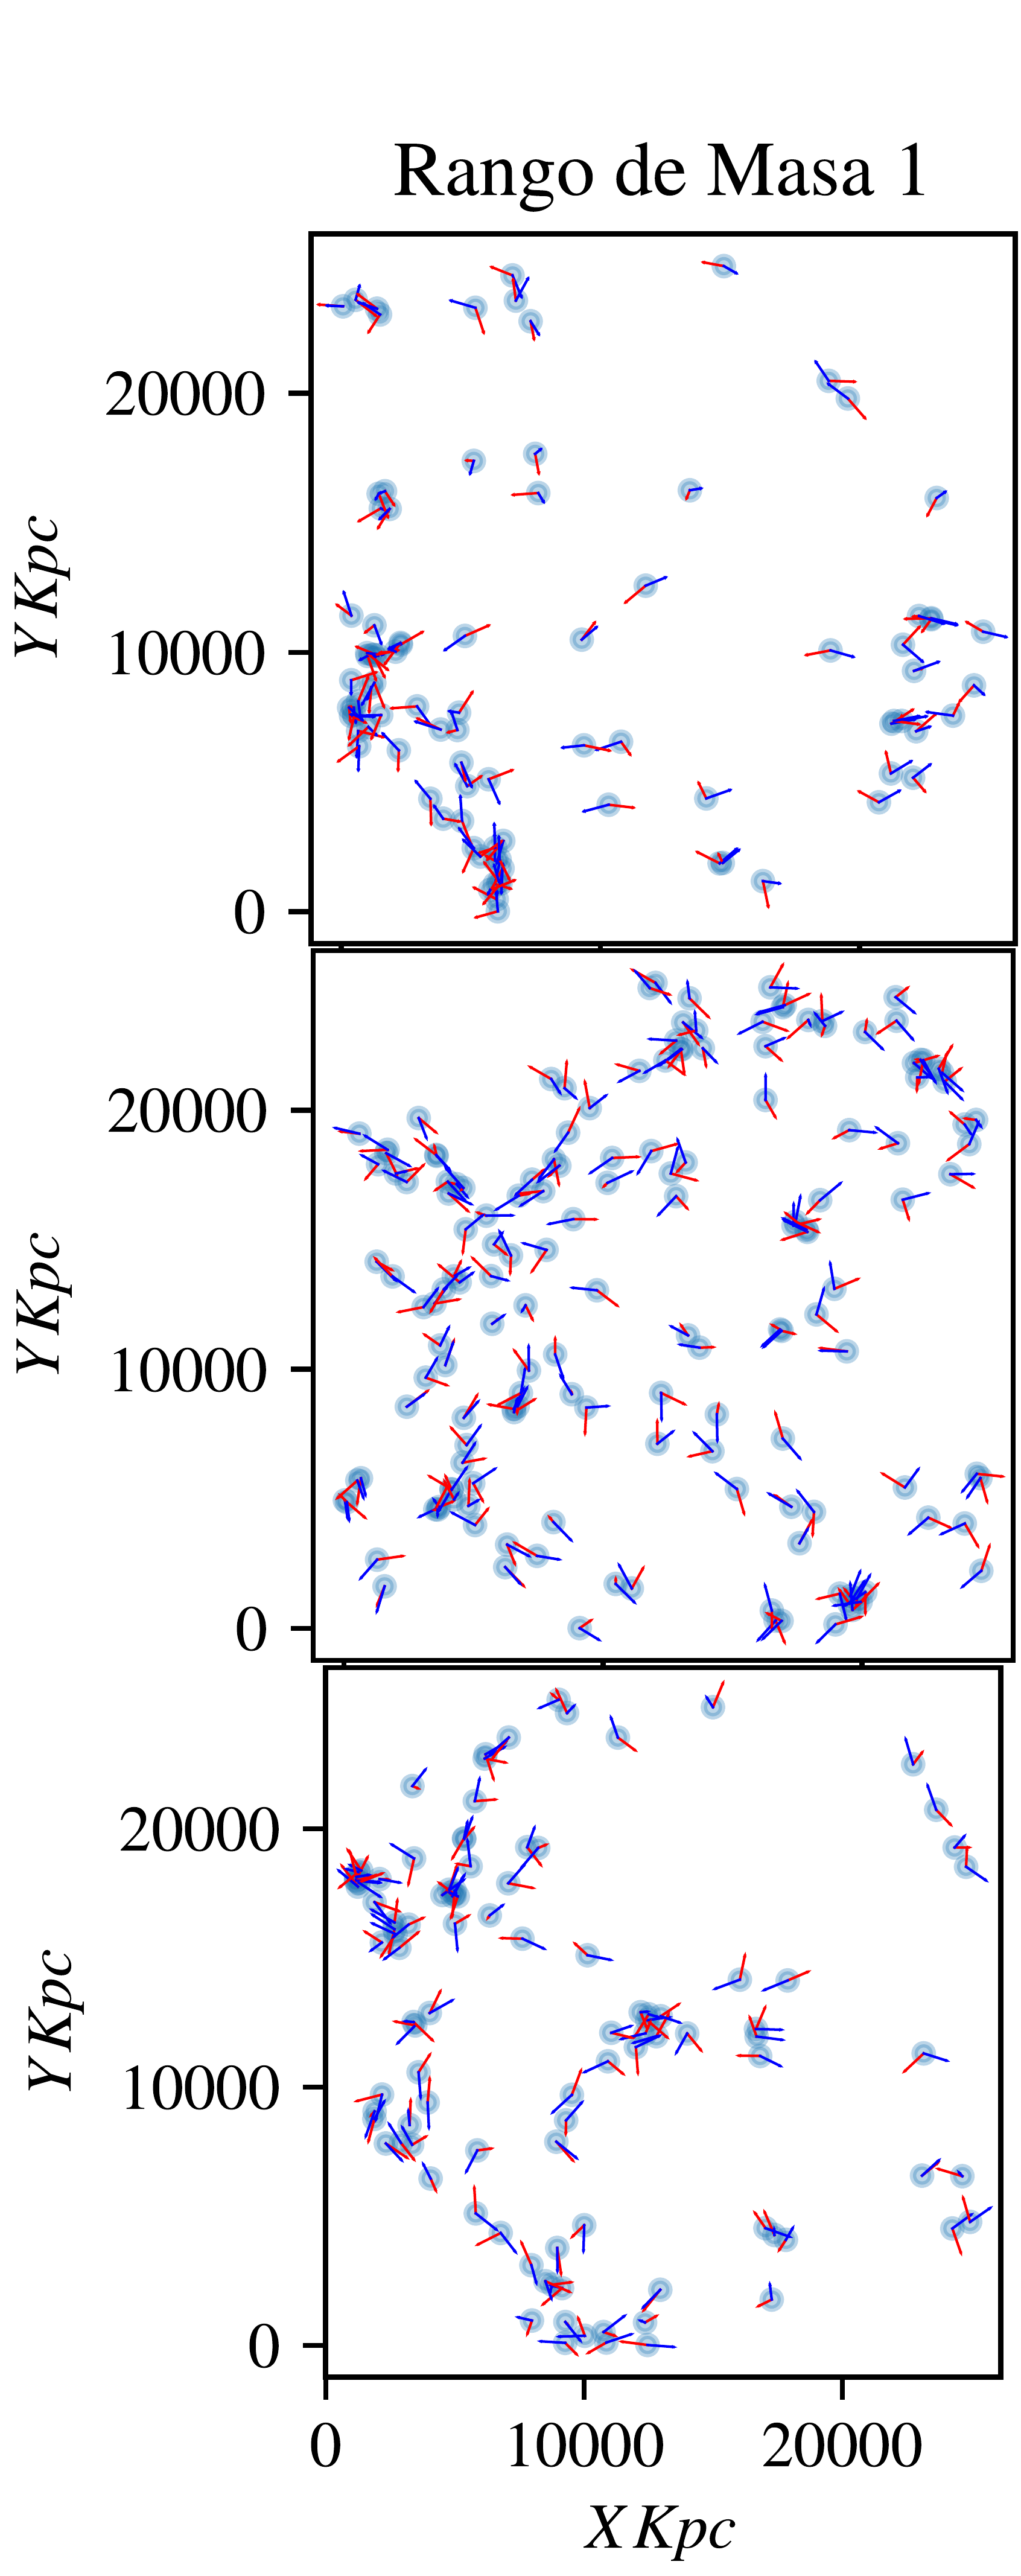
\includegraphics[width=0.38\textwidth]{./figures/6_Resultados/cosmo01/proyecion_rango_1_masas.png}} 
\subfloat{ 
%\label{fig: función de masa halos}
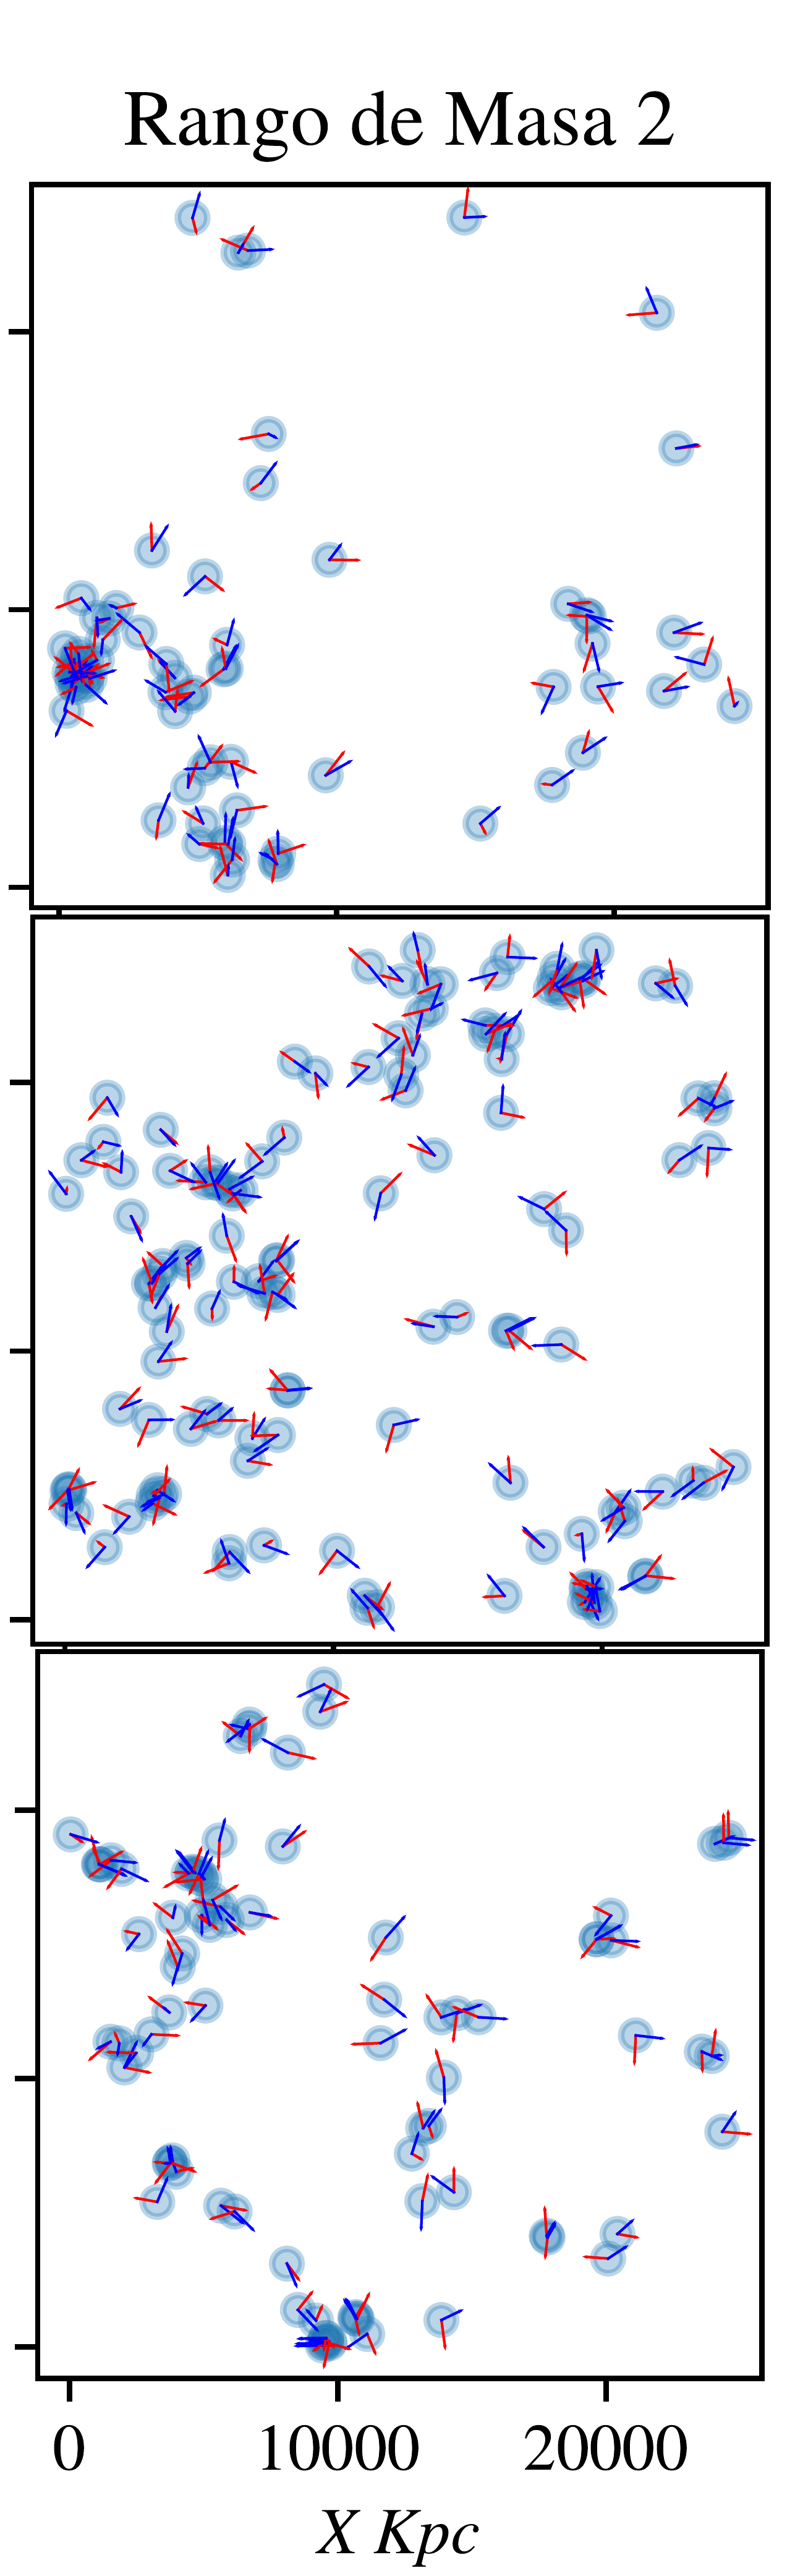
\includegraphics[width=0.29\textwidth]{./figures/6_Resultados/cosmo01/proyecion_rango_2_masas.png}}
\subfloat{
%\label{fig: función de masa estelar}
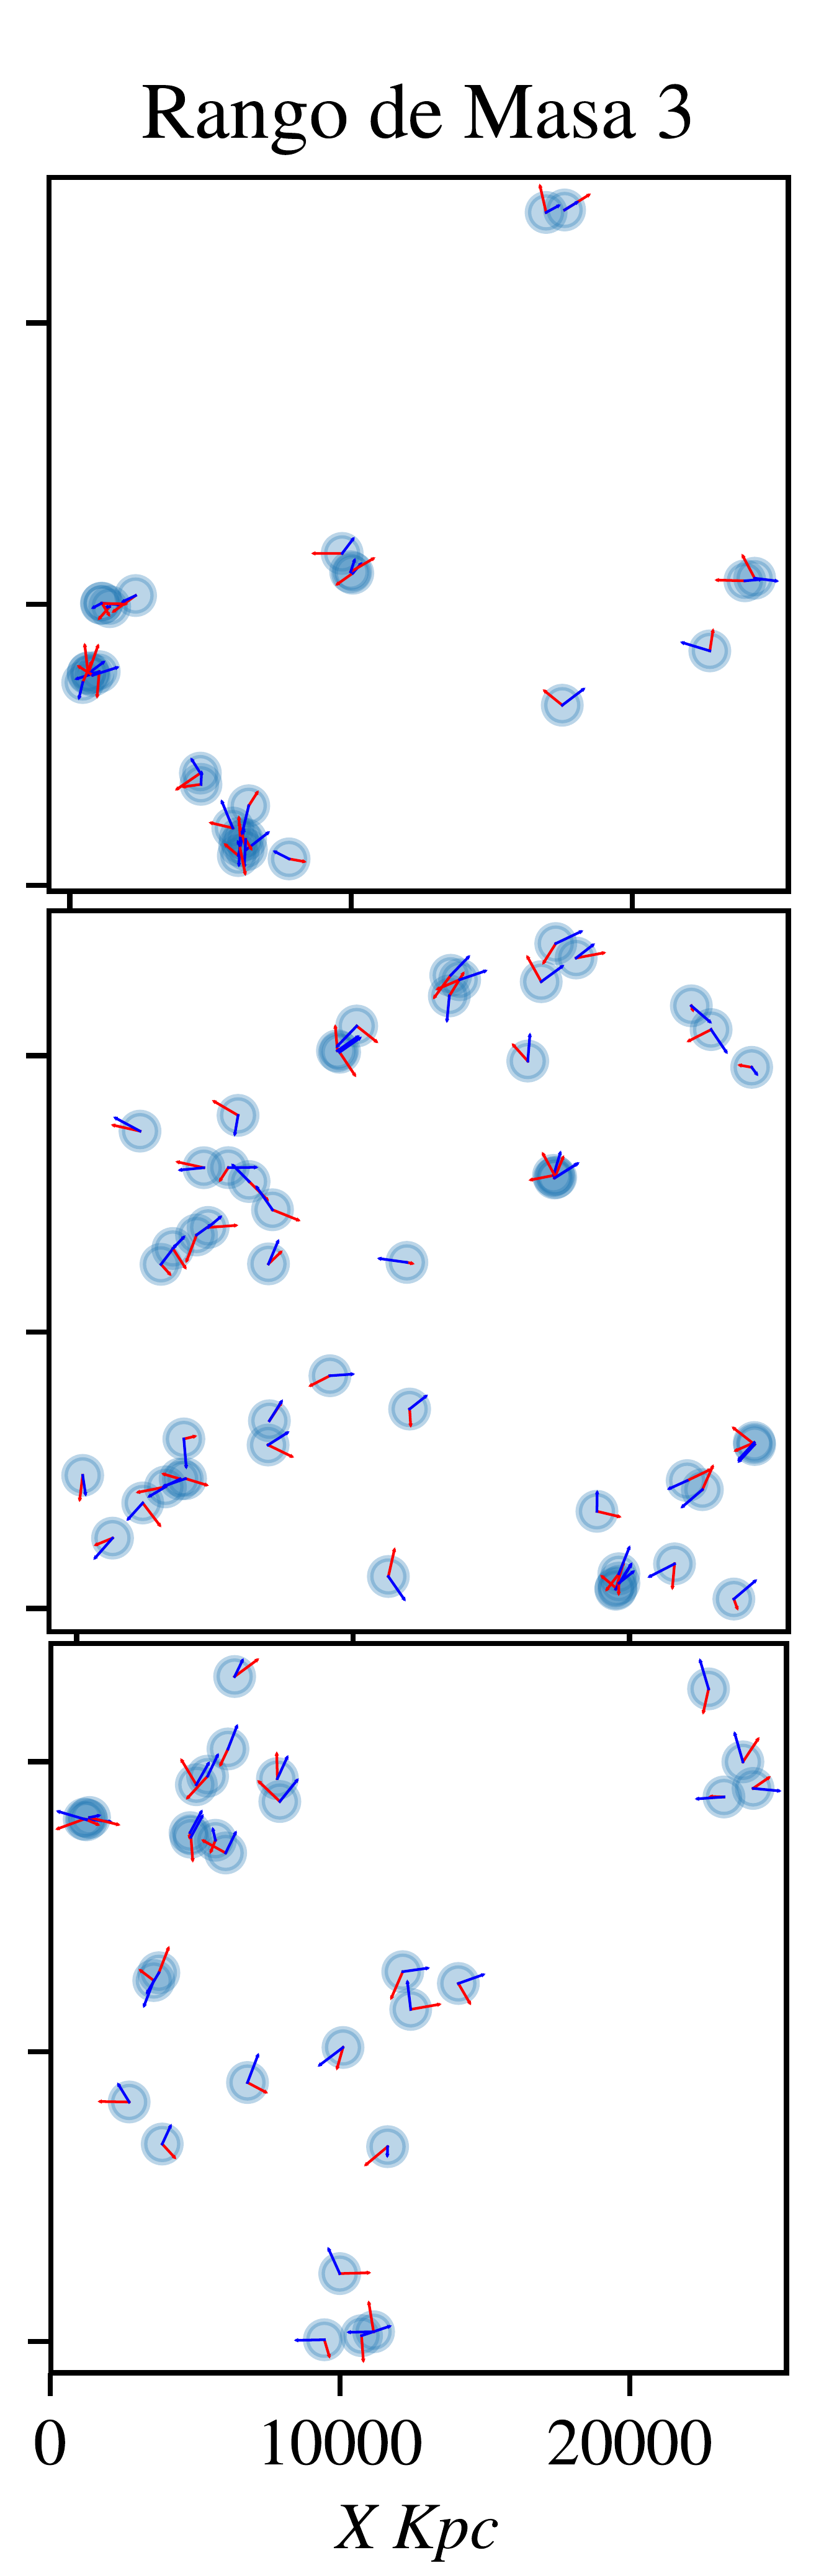
\includegraphics[width=0.302\textwidth]{./figures/6_Resultados/cosmo01/proyecion_rango_3_masas.png}} 
\caption{\emph{Representación de la correlación entre el autovector tres ${\bf{\vec{e}}_{3}}$ (Azul) y el espín del BH ${\bf{J_{bh}}}$ (Rojo). En esta figura se proyectan los vectores en el plano $x,y$. La figura presenta tres columnas, cada una de ellas relaciona un rango de masas, Rango 1 equivale a masas de BHs entre ($10^6-10^7)M_{\odot}$, Rango 2 masas entre ($10^7-10^8)M_{\odot}$ y Rango 3 masas entre ($10^8-10^10)M_{\odot}$. Cada columna de rango consta de tres figuras, donde cada celda  representan tres cortes en la caja de la simulación, cortes hechos en el eje $z$, La primera fila indica un corte interior, BHs entre $(0-8.3)\times10^{3} kpc$,  la segunda fila un corte intermedio, entre $(8.3-16.6)\times10^{3} kpc$, la ultima fila representa el corte superior, entre  $ (16.6-25)\times10^{3} kpc$. }} 
\label{fig: proyeccion espines} 
\end{figure}

Para entrar a analizar el alineamiento se busca su posible relación con la masa o con el mismo autovalores $\lambda_{3}$. 
%(¿PONGO QUE EL ANALISIS PARA LOS OTROS TRES AUTOVALORES?).
La teoría de formación de estructuras ( sección \ref{subsec: Metodo_T-web}) indica que las regiones donde se forman filamentos está determinada por el valor del autovalor 3 $\lambda_{3}$, al estudiar la dinámica del flujo de materia en las estructuras, se estima  que en filamentos hay una mayor concentración de materia en una dirección, esto puede suponer que los objetos inmersos en esa región tienden a alinearse en la dirección del flujo de materia. No solo en los filamentos se debería esperar alguna alineación, se puede suponer que en regiones de alta densidad de materia, donde la materia apunta hacia una misma dirección debería ocurrir alguna alineación. La figura (\ref{fig: Histograma Autovalores}) indica que la mayoría de los BHs van a estar en filamentos o clusters. 

\begin{figure}
    \centering
    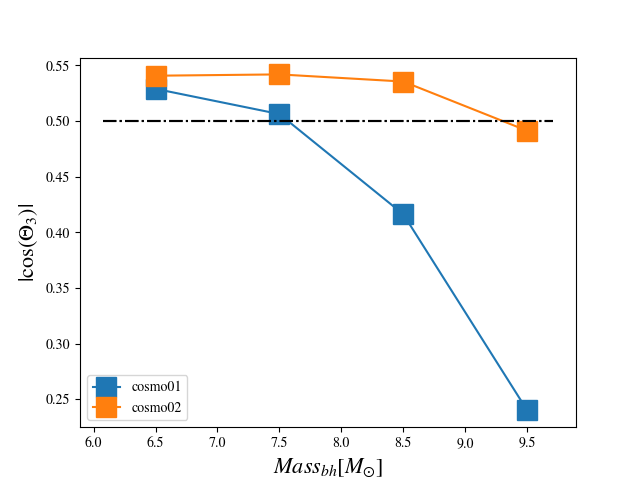
\includegraphics[width=0.6\textwidth]{./figures/6_Resultados/cosmo01/percentiles/relacion_simulaciones_Mass_bh}
    \caption{\emph{Alineamiento entre el espín del BH y autovector $\vec{\bf{e}}_3$ en función de $M_{bh}$. Se hace una comparación entre los datos obtenidos usando los dos regímenes. La linea y puntos azules son el resultado del régimen caótico, las líneas y puntos naranjas son el resultado para el régimen coherente.}}
    \label{fig: comparacion cosmo01 y cosmo02}
\end{figure}
 
Uno de los criterios por los cuales no se estudio {\it{cosmo02}}, son lo resultados logrados por su proceso de acreción coherente, no se logra constatar un claro  alineamiento. Al observar la figura (\ref{fig: comparacion cosmo01 y cosmo02}) se puede evidenciar que la mediana de los diferentes rangos de masas de los BHs para la simulación {\it{comos01}} siempre está muy cercano de 0.5, con lo cual no es posible concluir algo, mientras que para la simulación {\it{cosmo01}} si hay un cambio, una tendencia hacia el alineación. 

La figura (\ref{fig: median dispercion}) representa el resultado final de este trabajo. Se presentan cuatro  figuras, cada figura contiene a su vez dos gráficas, la gráfica superior de cada figura muestra la mediana para un rango de datos ($\lambda_{3}, M_{bh}, M_{halo}, M_{estelar}$), además se muestra los percentiles al 25$\%$ y 75$\%$, que brinda información de la distribución de la mediana para cada rango de datos; la gráfica inferior muestra los valores de la  mediana para cada rango.
%voy acala primera da información de la mediana de los datos ($\lambda_{3}, M_{bh}, M_{halo}, M_{estelar}$) para cada rango de masa o de autovalor. 

Se evidencia que el valor del $|\cos \theta|$ varia con respecto a la masa, a medida que aumenta la masa de los objetos, la distribución apunta a un alineamiento ortogonal entre el entorno y las masas. Se observa en especial, que el mayor alineamiento ocurre entre el entorno y la masa del BH, para BHs muy masivos $|\cos\theta| \to 0.2$. Contrastando este resultados con \cite{wang2018}, que estudia la relación del entorno con el espín del halo, los resultados finales de nuestra simulación son capaces de reproducir su resultado, dando  respaldo a la simulación y al modelo.

Entonces, se puede afirmar que la dinámica del entorno o de las  estructuras a gran escala si afecta los procesos internos en las galaxias. El campo de densidad que fluye a través de los filamentos o clusters influyen en la dirección del espín del BH. Por tanto el espín del BH ${\bf{J_{bh}}}$ se alinea de forma ortogonal con el autovector tres $\vec{\bf{e}_3}$ para masas grandes. 
%
%\begin{align}
% |\cos \theta| =   \left\| \frac{{\bf{J_{bh}}}\cdot \vec{\bf{e}_3}}{ %|\bf{J_{bh}}| |\vec{\bf{e}_3}|} \right\| \to 0.2
%\end{align}

\begin{figure} 
\centering 
\subfloat{
%\label{fig: función de masa estelar}
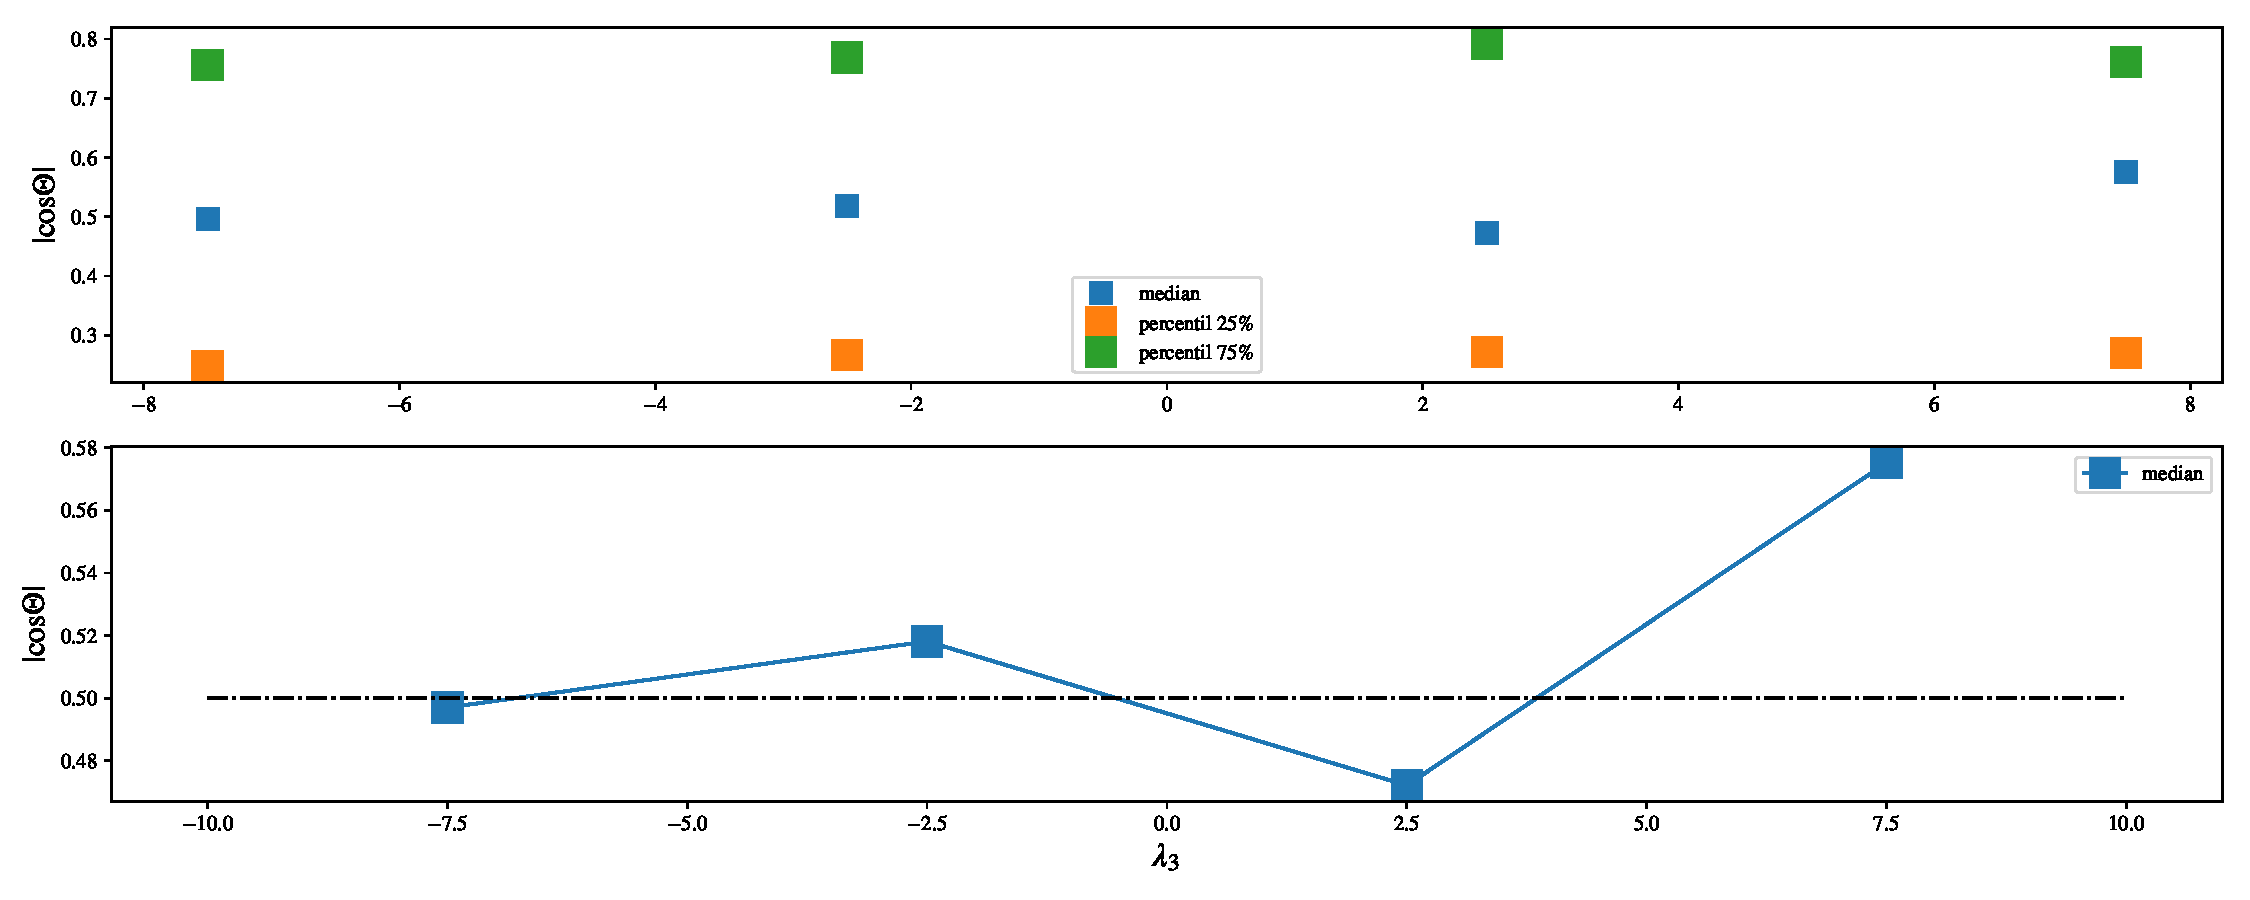
\includegraphics[width=0.63\textwidth]{./figures/6_Resultados/cosmo01/percentiles/mean_cos_theta3_vs_eigen3_bin4.pdf}} 
\subfloat{ 
%\label{fig: función de masa BHs}
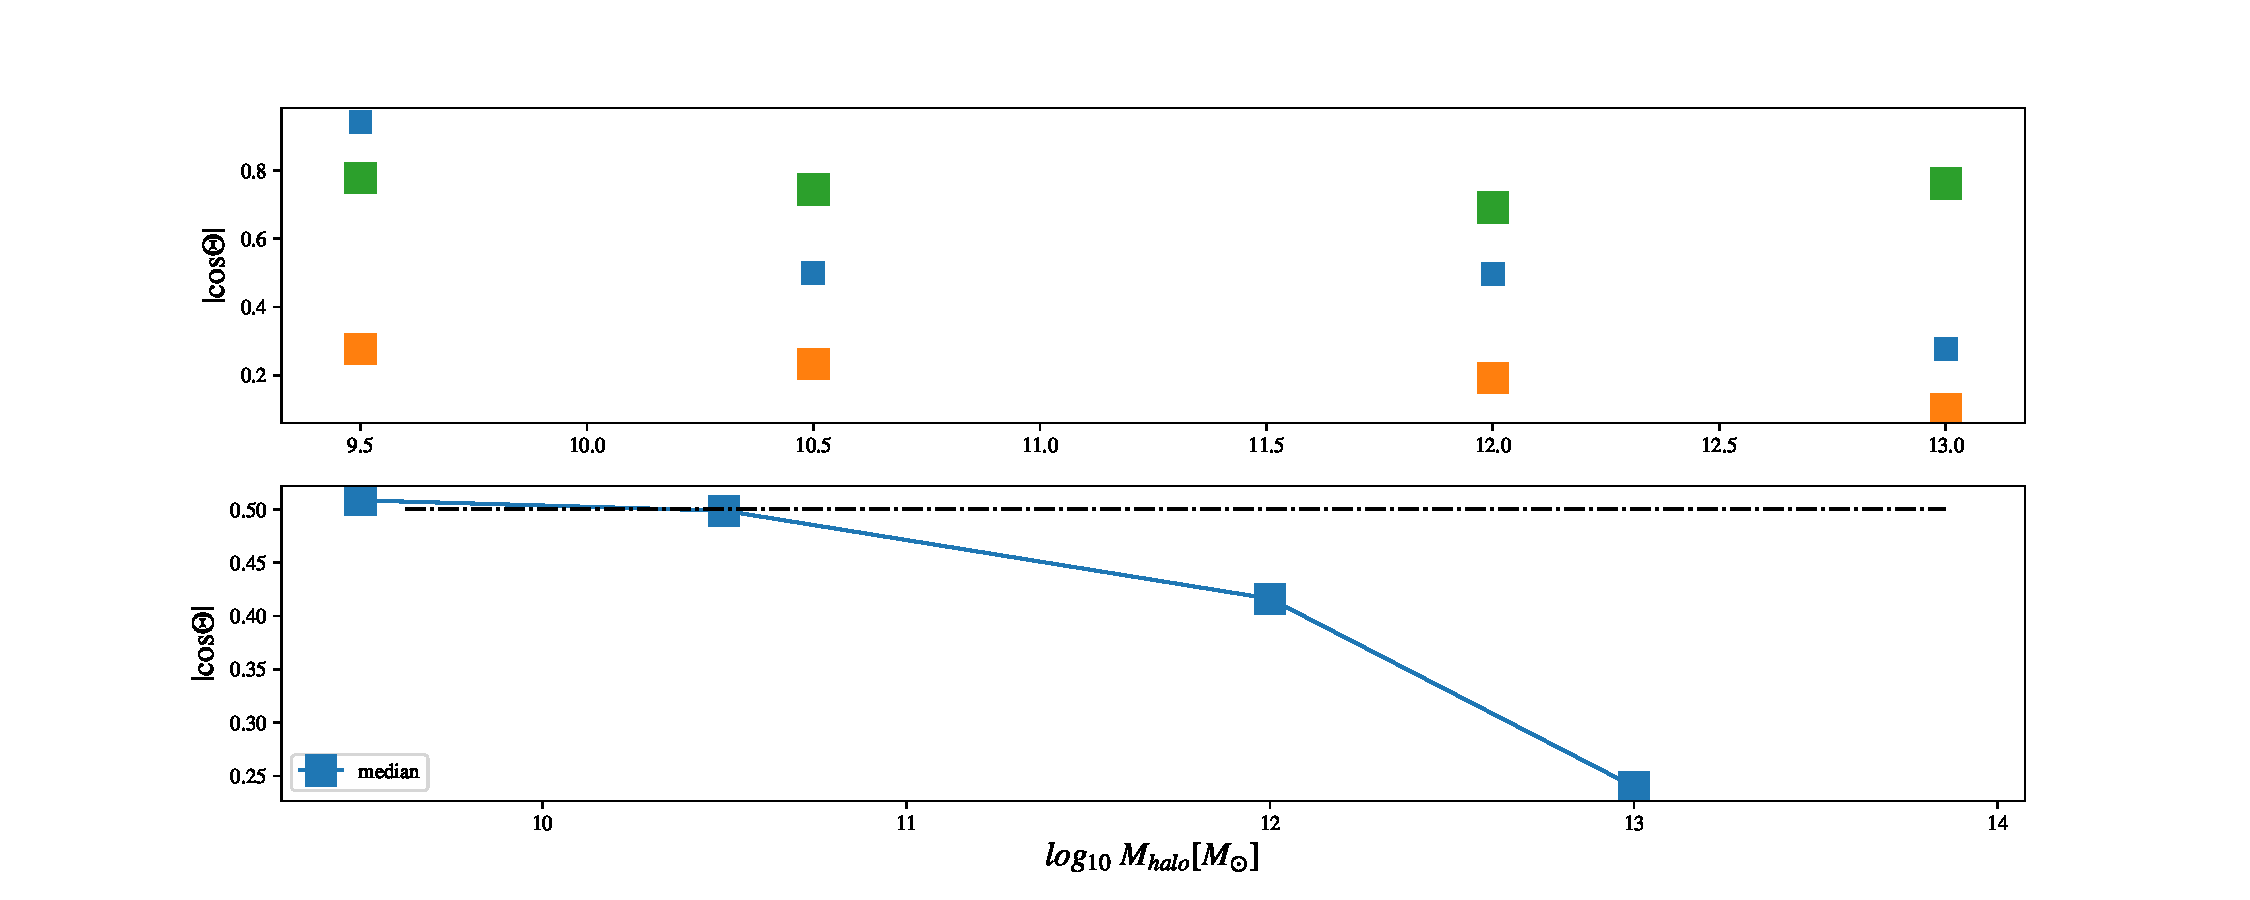
\includegraphics[width=0.77\textwidth]{./figures/6_Resultados/cosmo01/percentiles/mean_cos_theta3_vs_Mass_halo_bin4}} 
\subfloat{ 
%\label{fig: función de masa halos}
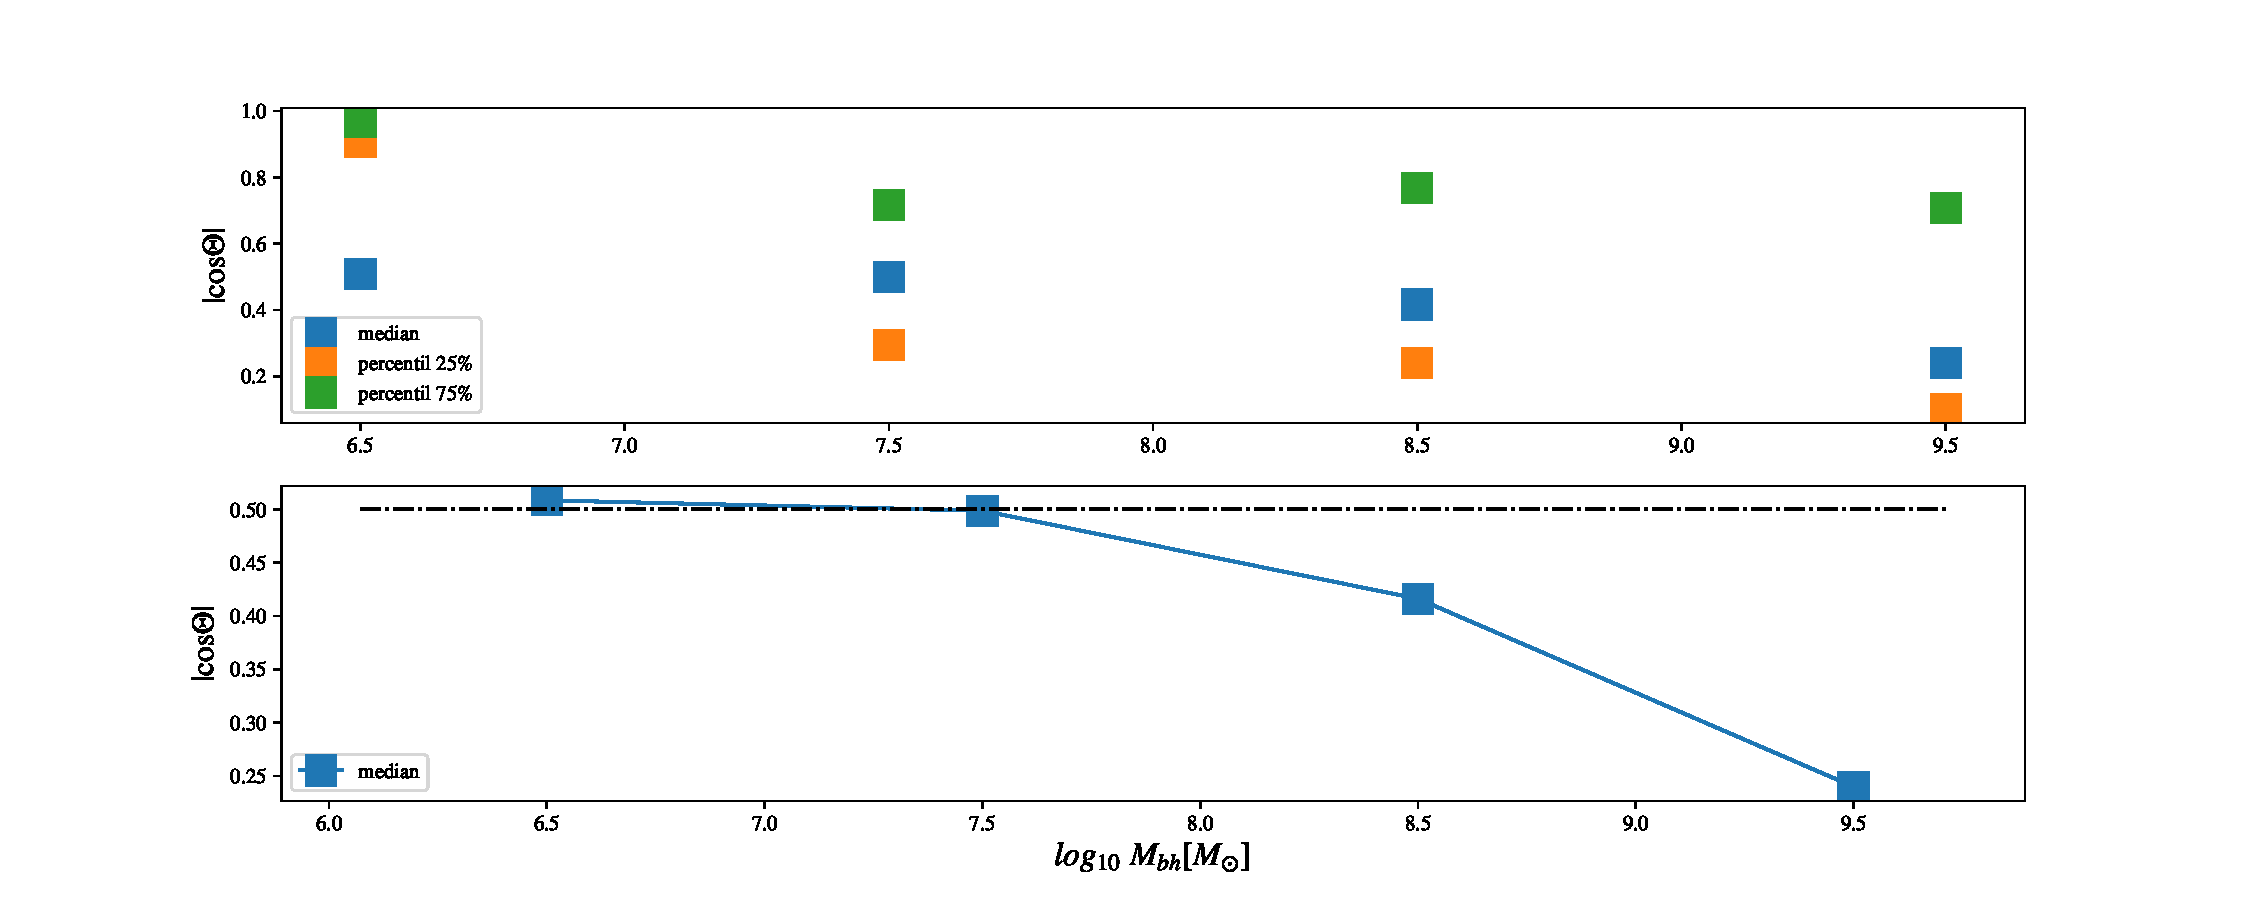
\includegraphics[width=0.77\textwidth]{./figures/6_Resultados/cosmo01/percentiles/mean_cos_theta3_vs_Mass_bh_bin4.pdf}}
\subfloat{
%\label{fig: función de masa estelar}
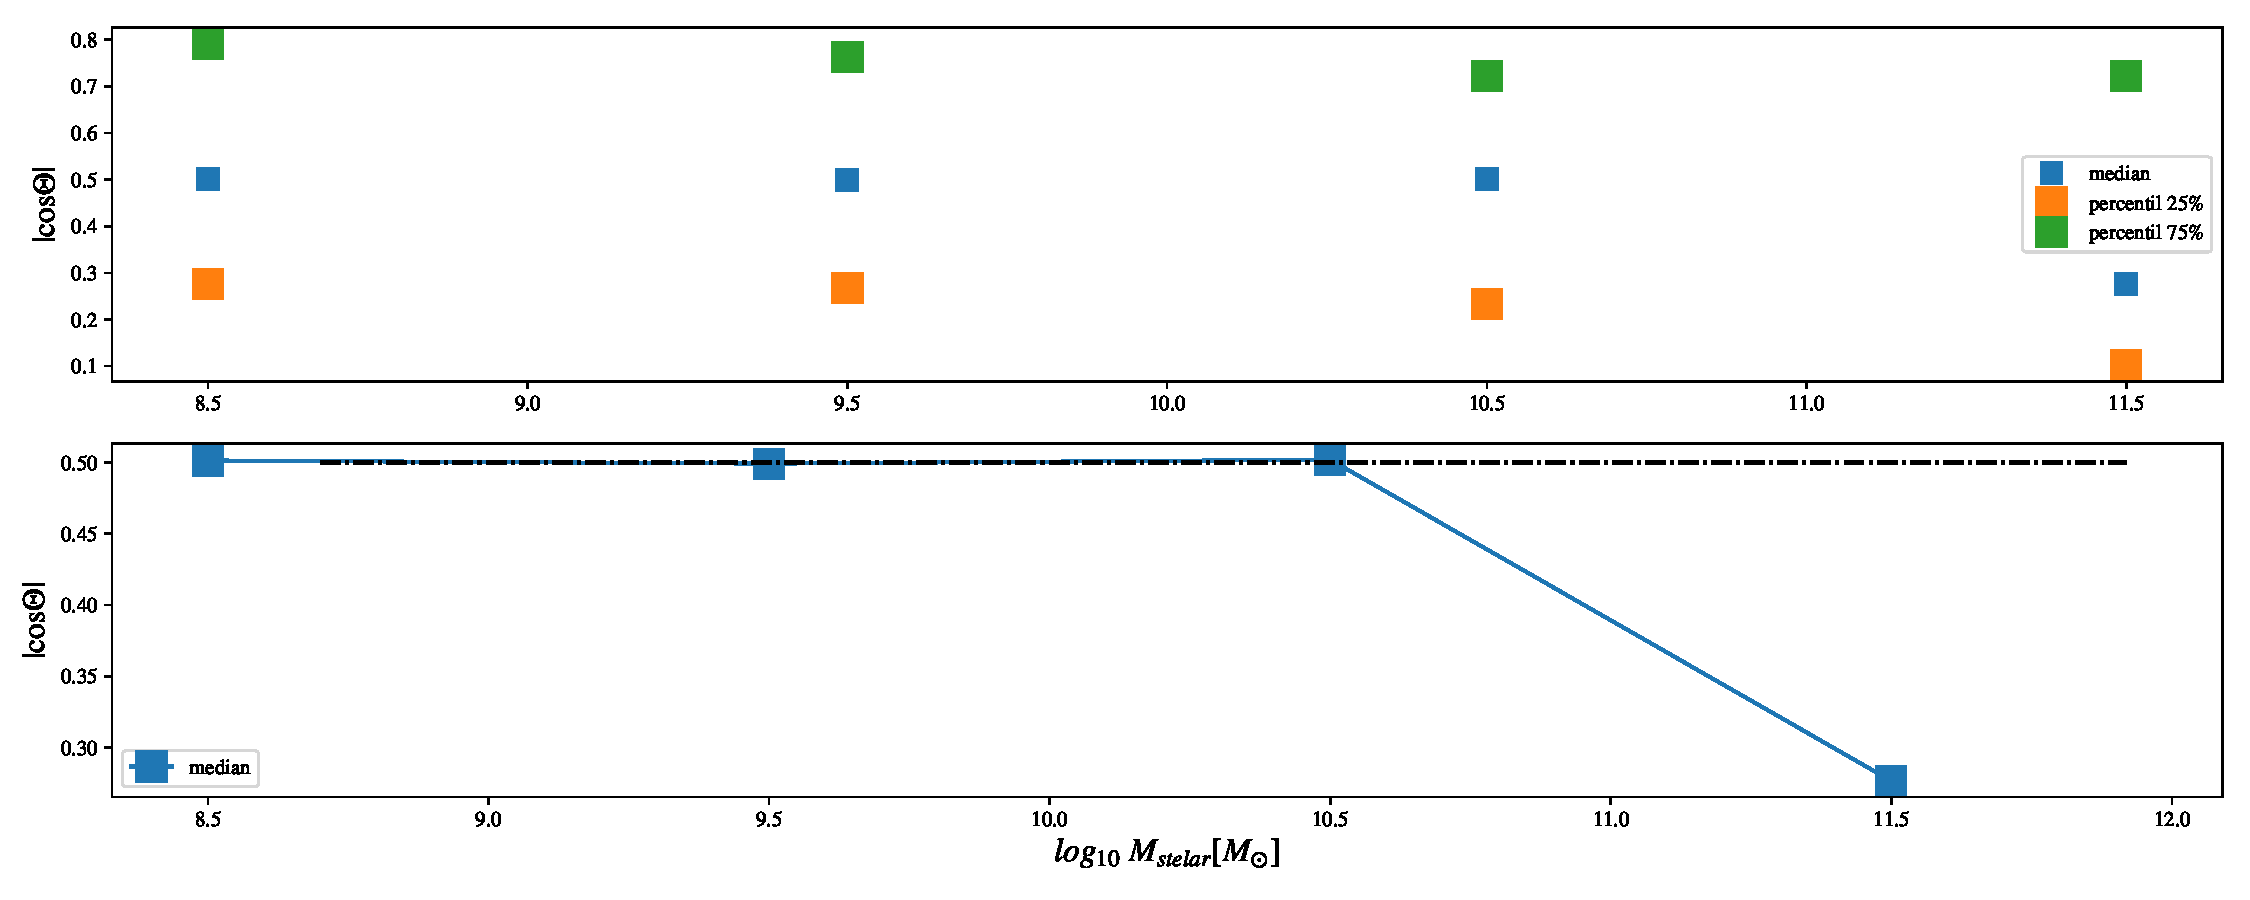
\includegraphics[width=0.63\textwidth]{./figures/6_Resultados/cosmo01/percentiles/mean_cos_theta3_vs_Mass_stelar_bin4.pdf}} 
\caption{\emph{Alineamiento entre el espín del BH y autovector $\vec{\bf{e}}_3$ en función de las variables ($\lambda_{3}, M_{bh}, M_{halo}, M_{estelar}$). Se tienen 4 figuras, cada figura contiene dos gráficas, las gráficas superiores muestran el valor de la mediana para varios rangos de datos, donde además se muestra los percentiles al 25$\%$ y 75$\%$. la gráfica inferior muestra solamente los valores de la mediana para cada rango.} }
\label{fig: median dispercion} 
\end{figure}


\newpage
%------------------------------------------------
\section{Anexos}
\label{sec: anexos}
%------------------------------------------------
(GRAFICAS HISTOGRAMAS DE ALPHA Y BETA)

Durante la realización de este trabajo se analizaron una variedad de eventos, eventos encaminados en alineamientos entre diferentes sistemas (BH, halos y discos de acreción). En este sección se presentaran los resultados obtenidos y el respectivo análisis.



%(1. Mostrar las relaciones con los percentiles )
%(2. Concluir con respecto a esas gráficas)
%(3. Con respecto a la conclusiones de las graficas de percentil volver a la gráfica de proyección y dar un análisis)

\newpage
%------------------------------------------------
\section{Conclusiones}
\label{sec: conclusiones}
%------------------------------------------------
%En esta sección se presentan los resultados obtenidos durante este trabajo,  los cuales serán presentados a continuación: 
Durante todo este trabajo, se ha encaminado en un objetivo específico, encontrar un posible alineación entre el entorno cosmológico y los AGNs. En esta sección se mostraran los resultados obtenidos a lo largo de este trabajo.

%$\bullet$ El modelo de espín [SEBAS], desempeña un papel fundamental en el alineamiento de los BHs. 

En este trabajo se presento un modelo de evolución de espín, a partir del cual se pretende encontrar algún tipo de alineación entre el entorno cosmológico y la orientación del AGN. Se hizo uso de las simulaciones cosmológicas hidrodinámicas The Illustris TNG. El criterio de alineamiento está basado en el valor obtenido del $|\cos \theta|$ para diferentes variables en la simulación ($\lambda_{3}, M_{bh}, M_{halo}, M_{estelar}$). 

Al usar los datos obtenidos de las simulaciones {\it{cosmo01}} y {\it{cosmo02}} se evidencia que los procesos que ocurren bajo la acreción caótica dan cuenta de un alineamiento más contundente, en especial para la masa. Para la acreción coherente no se evidencia un posible alineamiento, los resultados no permiten concluir. 

Inspeccionando las figuras (\ref{fig: proyeccion espines} y \ref{fig: median dispercion}) es posible afirmar que existe una relación entre la masa y el ángulo de alineamiento, se observa una mayor alineación para la masa de los BH. La figura (\ref{fig: median dispercion}) deja ver que para los BH más masivos, la dirección del campo de densidad y la orientación del espín del BH tiende a ser ortogonal. 

Del resultado anterior se puede concluir que hay un posible alineamiento entre la masa y el espín del BH. Debido a la relación que existe entre la masa y el entorno, se puede concluir por tanto que si hay evidencia que apunta a un alineamiento entre el entorno cosmológico y la orientación del AGN. Se podría afirmar que el flujo de materia que circula por las estructuras, sí afecta la orientación de los AGNs y esto se observa en una gran medida para AGNs muy masivos.
%Por lo tanto, se puede decir que se ha encontrado  ha logrado encontrar un alineamiento 


%***********************************************************************





% --------------------------------------------------------------
%:                  BACK MATTER: appendices, refs,..
% --------------------------------------------------------------

\backmatter


%: ----------------------- bibliography ------------------------



%\cite{*}
%\bibliographystyle{abbrv}

\bibliographystyle{plainnat}
%\bibliographystyle{abbrvnat}
%\bibliographystyle{acm}
\bibliography{chapters/ref.bib}

%\printnomenclature 
% --------------------------------------------------------------



\end{document}